\documentclass[a4paper,11pt]{book}
\usepackage[T1]{fontenc}
\usepackage[utf8]{inputenc}
\usepackage{gfsbodoni}
\usepackage[showframe]{geometry}

\usepackage{textcomp}
\usepackage{lmodern}
\usepackage[italian]{babel}

\usepackage{graphicx}


\DeclareUnicodeCharacter{B0}{\textdegree}


\title{De Angeli Frua Un secolo di tessuti}
\author{Loredano Tavazzi}

\begin{document}

% \maketitle
% \tableofcontents

\begin{titlepage}
{\centering
  \fontfamily{gfsbodoni}
  \fontseries{m}
  \fontshape{n}
  \fontsize{2cm}{1cm}
  \selectfont
De Angeli Frua
  \par
}
\vspace{1cm}
{\centering
\fontsize{2cm}{1cm}
  \selectfont
De Angeli Frua
  \par
}

\end{titlepage}

\clearpage

\clearpage
\chapter*{Ringraziamenti}

SI RINGRAZIANO 
PER AVERE OFFERTO NOTIZIE 
E DOCUMENTAZIONI:


Il dott. Dirk Ziezing per i testi in inglese e tedesco dedicati ai fazzoletti di istruzione militare e relativi documenti, usati dagli eserciti britannico e italiano.

Tutte le persone che hanno fornito informazioni e materiali utili alla compilazione del volume.









Gli estensori dei testi si scusano per eventuali imprecisioni anche nelle didascalie delle immagini.

L’ editore, pur avendo fatto il possibile per evitarli, si scusa per possibili errori od omissioni nella citazione delle fonti ed è a disposizione degli aventi diritto.

\clearpage

\clearpage
\chapter*{Premessa}
\graphicspath{ {./images/primepagine/} }

di Marina Frua

“Memorie della De Angeli Frua che meritano di essere conosciute e trasmesse”

\begin{figure}[h]
	\centering
		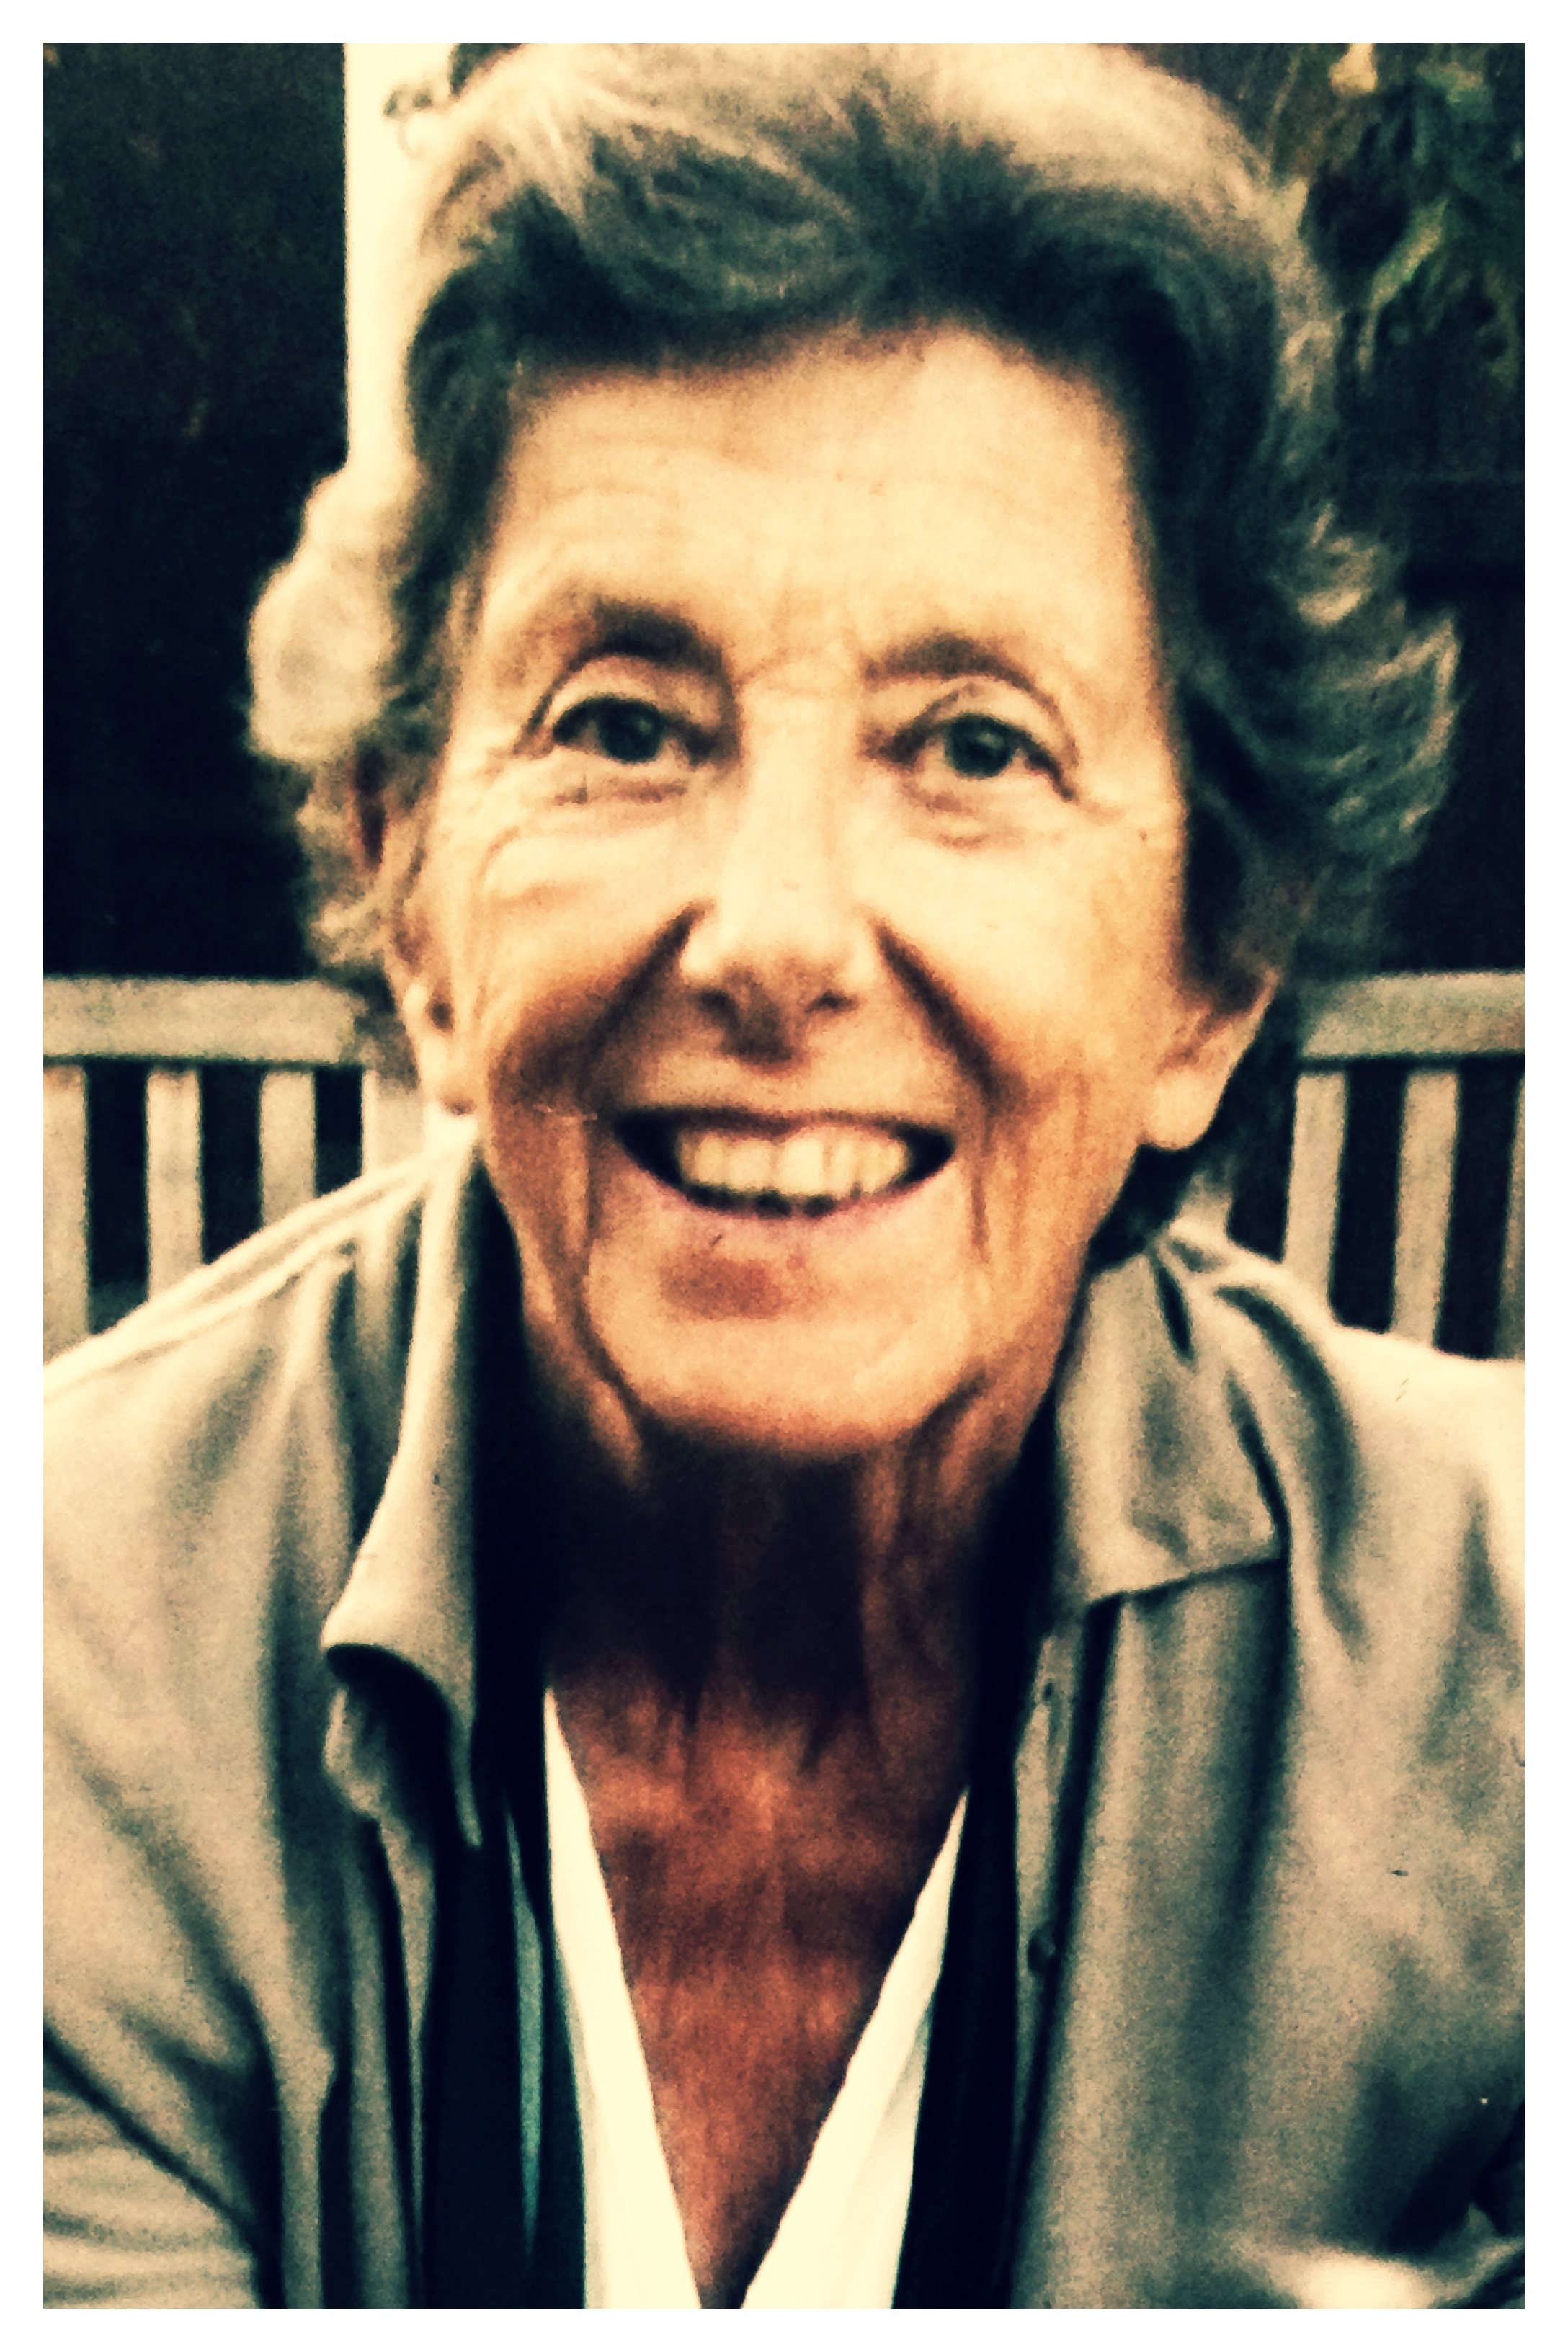
\includegraphics[width=\textwidth]{marina_frua.jpg}
	\caption{}
	\label{fig:marina_frua}
\end{figure}

A Milano in via Paleocapa al numero uno, una bella casa di quattro piani vicino alla Stazione Nord e al Parco Sempione, abitavano i De Angeli e i Frua.
   Ernesto De Angeli, senatore del Regno, e le sue belle, severe e impettite sorelle occupavano il primo e il secondo piano. Giuseppe Frua abitava al terzo piano e Alberto, figlio di Giuseppe, al quarto.
   Io facevo parte della famiglia di Alberto: ero piccola e di questi personaggi, all’epoca così importanti, ho un ricordo forse un po’ sbiadito ma a tratti intenso. 
   Sovente andavo a trovare mio nonno Giuseppe. Lui mi dava le arance affettate con lo zucchero e le violette candite e controllava che il mio vestitino fosse tassativamente di cotone: anche d’inverno. Ricordo il suo sorriso: con un lampo d’intesa i suoi occhi si accendevano di una luce speciale. Portava dei piccoli occhiali con una semplice montatura di metallo, per correggere il suo astigmatismo che qualcuno di noi ha ereditato.
   Il nonno Giuseppe era un grande lavoratore e ha trasmesso a tutti i suoi collaboratori la passione per il lavoro, l’amore per la famiglia, il rispetto per gli uomini e le cose, l’importanza dell’istruzione, dello studio e della religione. Aveva passato l’intera vita a creare con costanza e tenacia prodotti tessili di alta qualità in un’epoca in cui, all’estero, si diceva che l’Italia sapeva produrre solo arance e mandarini. Lui invece riuscì a far conoscere e apprezzare in tutta Europa i suoi tessuti fra i quali la famosa “Costella”, una stoffa dai piccoli disegni con il marchio “Sole e Onda”.
   Si occupava dei suoi collaboratori e operai come un padre e per loro creò abitazioni, asili e centri di assistenza sanitaria. Solo più tardi, crescendo, ho appreso quale impegnativo e prezioso lavoro ha fatto e quante drammatiche cose sono poi successe nella seconda guerra mondiale e nella difficile ripresa, con la distruzione e la chiusura delle fabbriche. Tutto disperso: filature, tessiture, stamperie, tessuti e storia. Si era dissolta anche la memoria.  
   Ma, nel quartiere Frua, le case di chi lavorava in fabbrica esistono ancora. E proprio in via Moncalvo abita e opera una persona che con tenacia ha voluto che il ricordo di tutto quel lavoro non andasse perduto: Loredano Tavazzi. Un personaggio eccezionale che ha passato una vita in quella via Moncalvo e che, ripensando ai valori creati e trasmessi da Giuseppe Frua, con passione intelligenza costanza e forse anche un pizzico di meritata fortuna, ha raccolto testimonianze e ha conservato ricostruito e descritto documenti che, altrimenti, sarebbero andati perduti. In questa sua ostinata ricerca ha recuperato, della De Angeli Frua, marchi, tessuti, fotografie, cartoline e manifesti pubblicitari.
   Ne è nato così questo volume – a seguito del precedente “De Angeli Frua, una famiglia, un’industria nella storia di Milano” – che evidenzia, tra le tante altre cose, la particolare scoperta, a molti credo sconosciuta, dei “fazzoletti militari” che rievocano momenti di storia europea pieni di guerre ma anche di analfabetismo. Forniti in dotazione ai soldati, questi fazzoletti illustravano con stampe e disegni attenti e dettagliati, sovente ricchi di vere soluzioni artistiche, come usare le armi ma poi come montare a cavallo o come disporsi sul campo.
   A Loredano Tavazzi va dunque il mio sentito e affettuoso ringraziamento e quello dei miei figli e nipoti che portano, oltre al proprio, il cognome Frua, per questo straordinario lavoro sulla conservazione di memorie della De Angeli Frua, che meritano di essere conosciute e trasmesse. 

Milano  2014

\begin{figure}[h]
	\centering
		
\includegraphics[width=\textwidth]{marina_frua_firma.jpg}
	\caption{}
	\label{fig:marina_frua_firma}
\end{figure}

\clearpage

\clearpage
\chapter[]{La nascita dei fazzoletti per istruzione militare}
\graphicspath{ {./images/chapter1/} }

\begin{figure}[h]
	\centering
		
\includegraphics[width=\textwidth]{britishEmpire.jpg}
	\caption{}
	\label{fig:britishEmpire}
\end{figure}

\newpage

I FAZZOLETTI CON ISTRUZIONI MILITARI 
    DELL’IMPERO BRITANNICO

   Quando il 19° secolo arrivò alla sua fine, strategie di guerra, tattiche e armamenti militari videro significativi cambiamenti. Questo fu il periodo della creazione dei fazzoletti illustrati,  allo scopo di fornire istruzioni militari e utili informazioni per il servizio militare e navale.
   Un ufficiale della fanteria dell’esercito Britannico ebbe l’idea di queste istruzioni militari illustrate su fazzoletti. Il suo nome è Carrè Fulton, nato il 15 marzo 1848 a Douglas, nell’Isola di Man, figlio gemello del Tenente-Colonnello William Fulton. Egli iniziò la sua carriera militare nel 1867 come fante del 15° Reggimento a piedi. Seguirono 3 anni di servizio oltremare in Giamaica e nelle Bermuda. Nel 1871 egli tornò in Gran Bretagna e fu promosso al grado di tenente e un anno dopo entrò a far parte del 68° Reggimento a piedi. Nel 1877 divenne capitano e nel 1883 maggiore, questa volta della fanteria leggera di Durham. Durante gli anni 1885 e 1886 egli servì  il corpo militare di frontiera di stanza in Sudan  e prese parte alla campagna contro le truppe della resistenza anticoloniale del Mahdi. 1 (vedi nota a pag. 36).
  Per la sua partecipazione alla battaglia di Ginnis, il 30 dicembre 1885 egli ricevette la medaglia per la campagna di Egitto insieme alla stella di Khedive. 
Fu dopo questa battaglia che le truppe Britanniche abbandonarono il classico colore rosso delle loro uniformi a favore del colore cachi, quale principio di una nuova era.
   Nel 1887, Fulton si ritirò con la carica di sottotenente-colonnello della fanteria leggera di  Durham.  Successivamente egli lavorò come poliziotto a Gibilterra. Al cambio del secolo, si sa che egli viveva nel quartiere di Acton a Londra, poiché il 16 novembre 1901 il Times menzionò il colonello Carrè Fulton in quanto vittima di una banda di ladri. Egli morì nel 1911 a Guernsey, un’isola del Canale della Manica. Suo figlio ventenne, il sottotenente Cecil John Fulton fu ucciso nell’aprile del 1916 e fu seppellito nel cimitero della città di Bethune (Francia).Carrè Fulton era un discendente di una famiglia di fabbricanti di stoffa. Nel 18° secolo il suo antenato Humphrey Fulton stabilì la manifattura della garza di seta in Scozia.

\newpage
   
\begin{figure}[h]
	\centering
		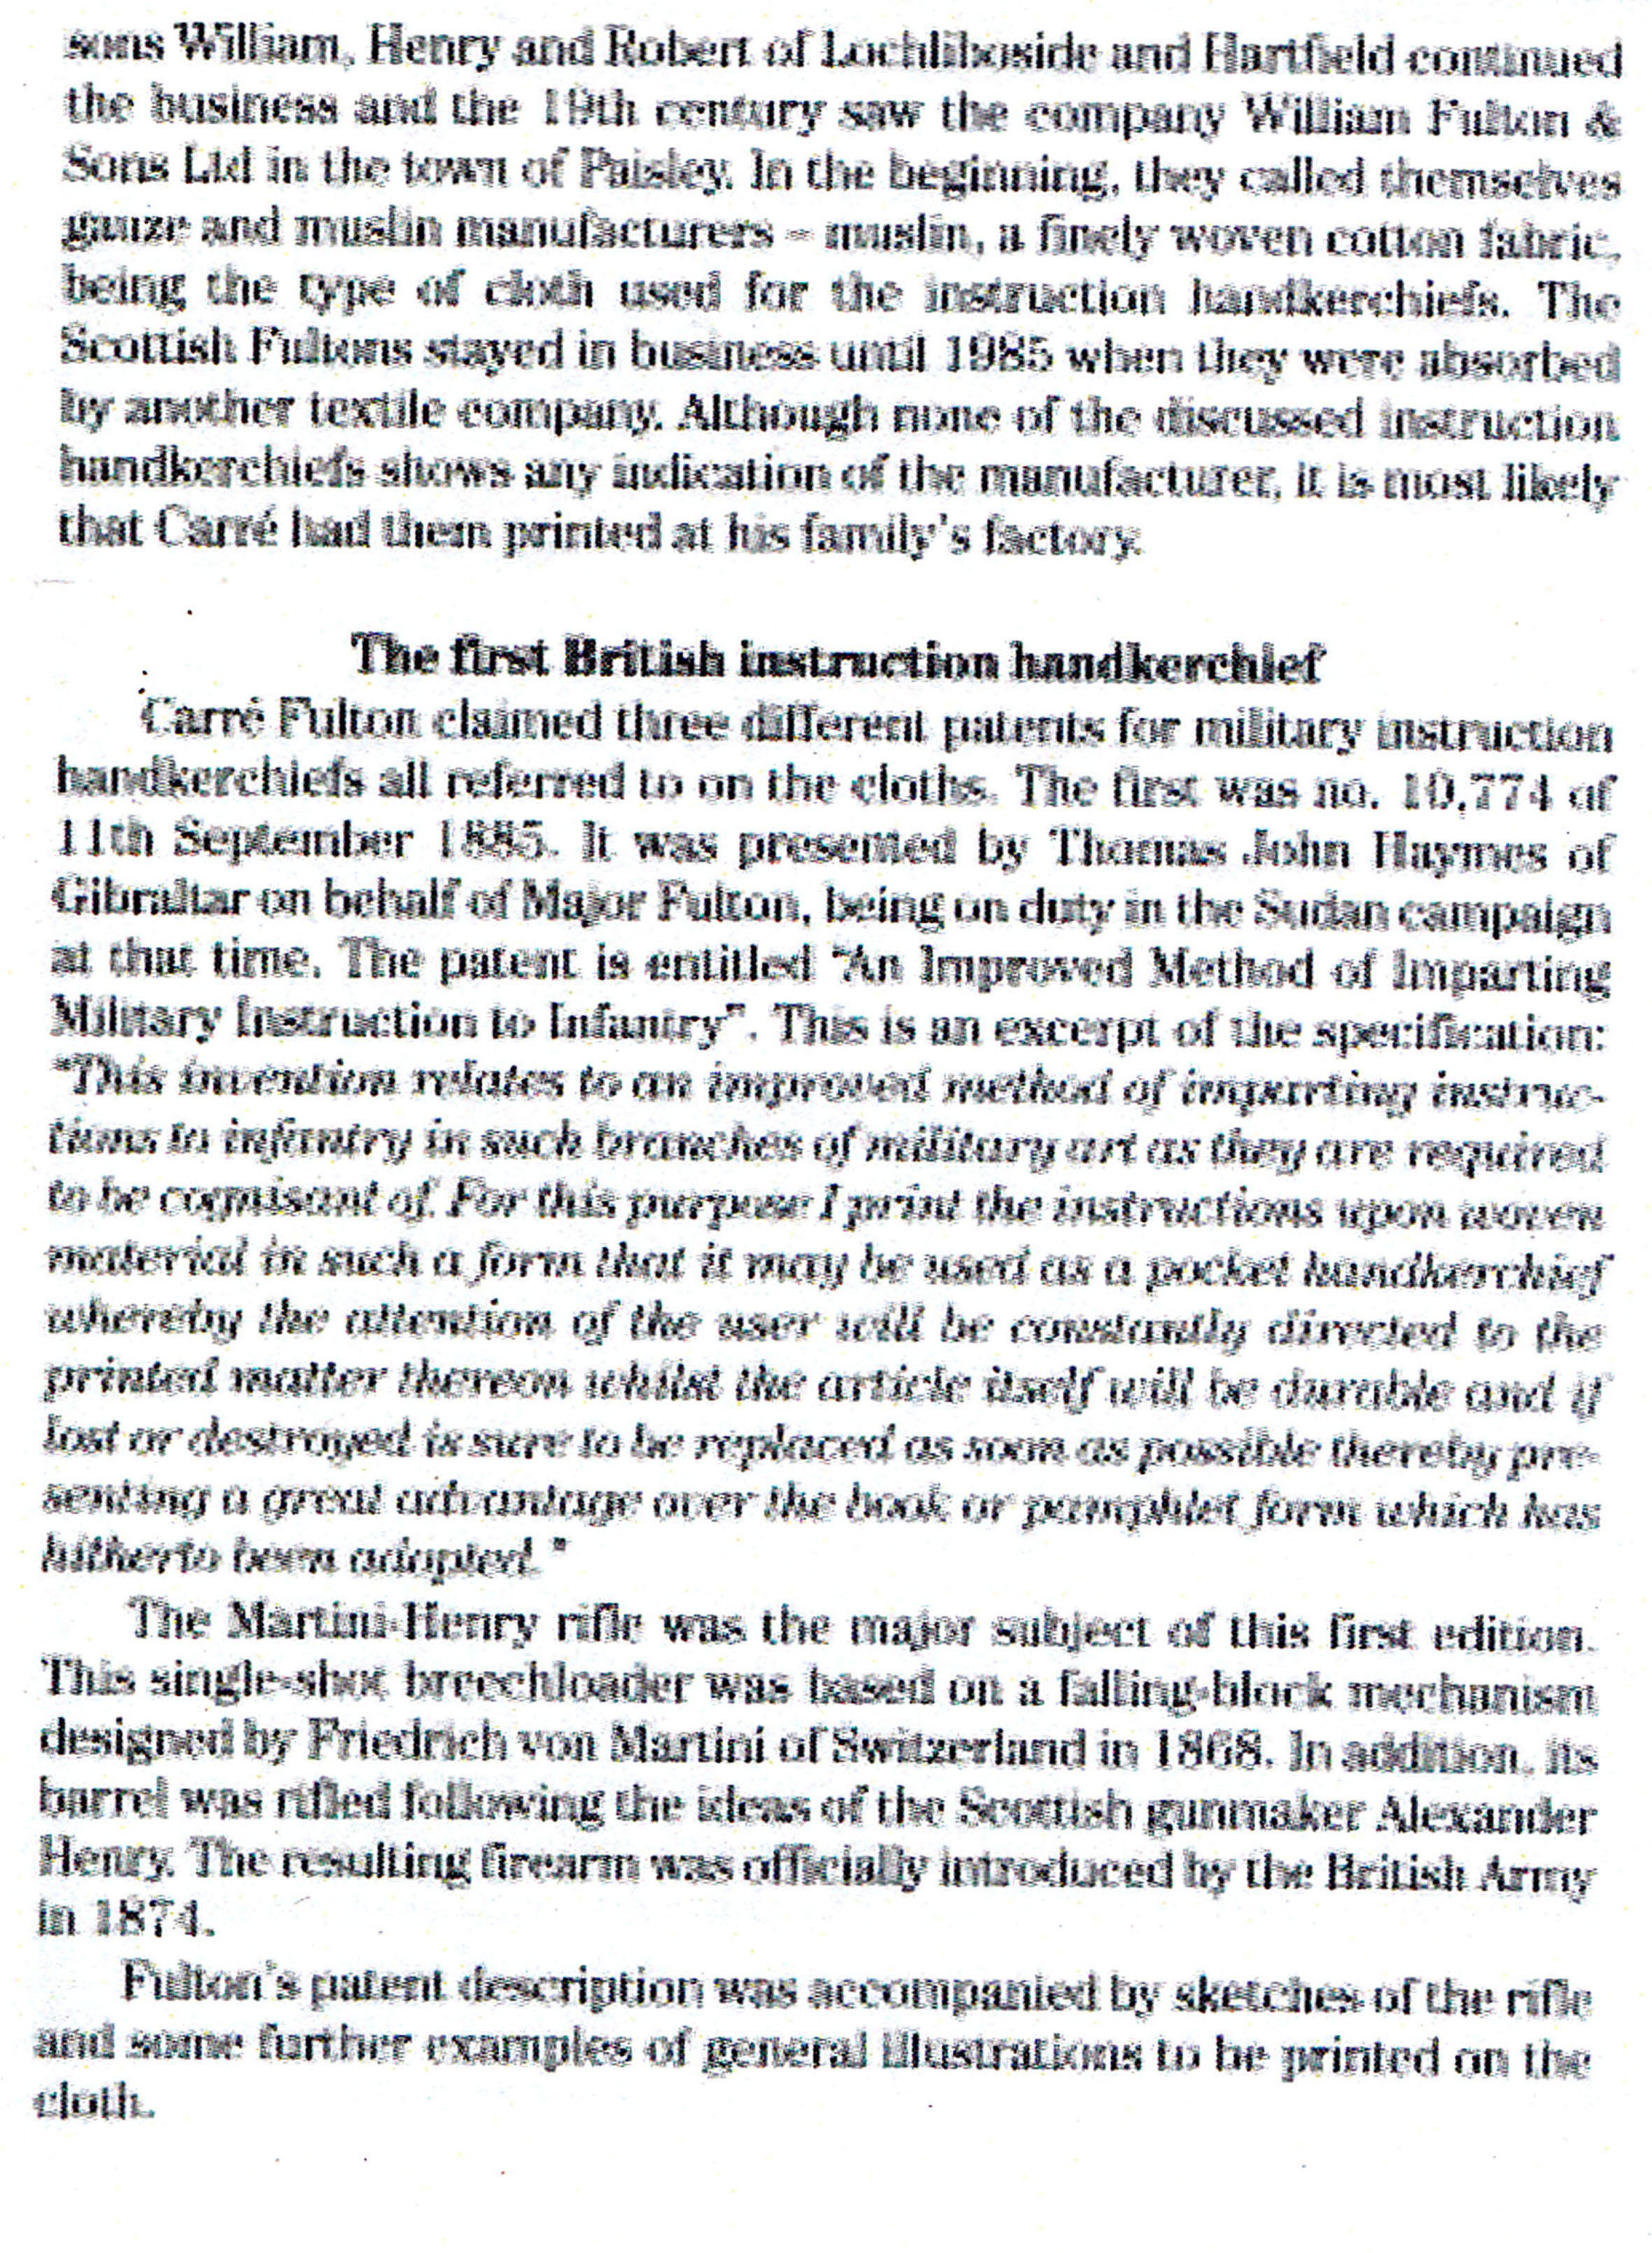
\includegraphics[width=\textwidth]{britishInstruct.jpg}
	\caption{}
	\label{fig:britishInstruct}
\end{figure}

\newpage

I figli di Humphrey, William, Henry e Robert di Lochliboside e Hartfield continuarono l’attività e il 19° secolo vide l’azienda William Fulton \& figli Ltd nella città di Paisley (Scozia). All’inizio essi si definirono produttori di garza e mussola; la mussola, un cotone intessuto finemente, divenne la stoffa  utilizzata per i fazzoletti con le istruzioni. Gli scozzesi Fulton mantennero l’attività fino al 1985 quando vennero acquisiti da un’altra società tessile. Malgrado nessuno dei citati fazzoletti con le istruzioni mostri alcuna indicazione del fabbricante, è molto probabile che Carrè li stampò nell’azienda di famiglia.

IL PRIMO FAZZOLETTO BRITANNICO CON ISTRUZIONI

   Carrè Fulton ottenne 3 diversi brevetti per le istruzioni militari sui fazzoletti, tutte stampate su stoffe. Il primo fu il n. 10.774 dell’11 settembre 1885. Questo fu presentato da Thomas John Hayrnes di Gibilterra al posto del Maggiore Fulton, impegnato nella campagna in Sudan a quel tempo. Il brevetto è intitolato “Un metodo migliore per impartire le Istruzioni Militari alla Fanteria”.  Questo un estratto della spiegazione: “ Questa invenzione si riferisce a un metodo migliore per impartire le istruzioni alla fanteria per quei rami dell’arte militare di cui devono essere a conoscenza. A questo scopo io stampo le istruzioni sopra il tessuto, in modo tale che possa essere  usato come fazzoletto tascabile. In questo modo l’attenzione dell’utilizzatore sarà costantemente diretta all’argomento stampato sino a quando l’oggetto in sé sia ancora utilizzabile e, in caso di perdita o distruzione, è sicuro che venga sostituito non appena possibile, rappresentando così un grande vantaggio rispetto al libro o l’opuscolo fin qui adottato.” 
   Il fucile Martini Henry fu il principale soggetto di questa prima edizione. Questo fucile a retro carica a colpo singolo fu basato su di un meccanismo di otturatore disegnato dallo svizzero Friedrich von Martini nel 1868. In aggiunta la sua canna fu rigata seguendo le idee del fabbricante di pistole scozzese Alexander Henry. L’arma da fuoco che ne risultò fu introdotta ufficialmente nell’esercito Britannico nel 1874.
   
\newpage

   
   

\clearpage
\chapter[]{I fazzoletti per istruzione militare in Italia}
\graphicspath{ {./images/chapter2/} }

\begin{figure}[h]
	\centering
		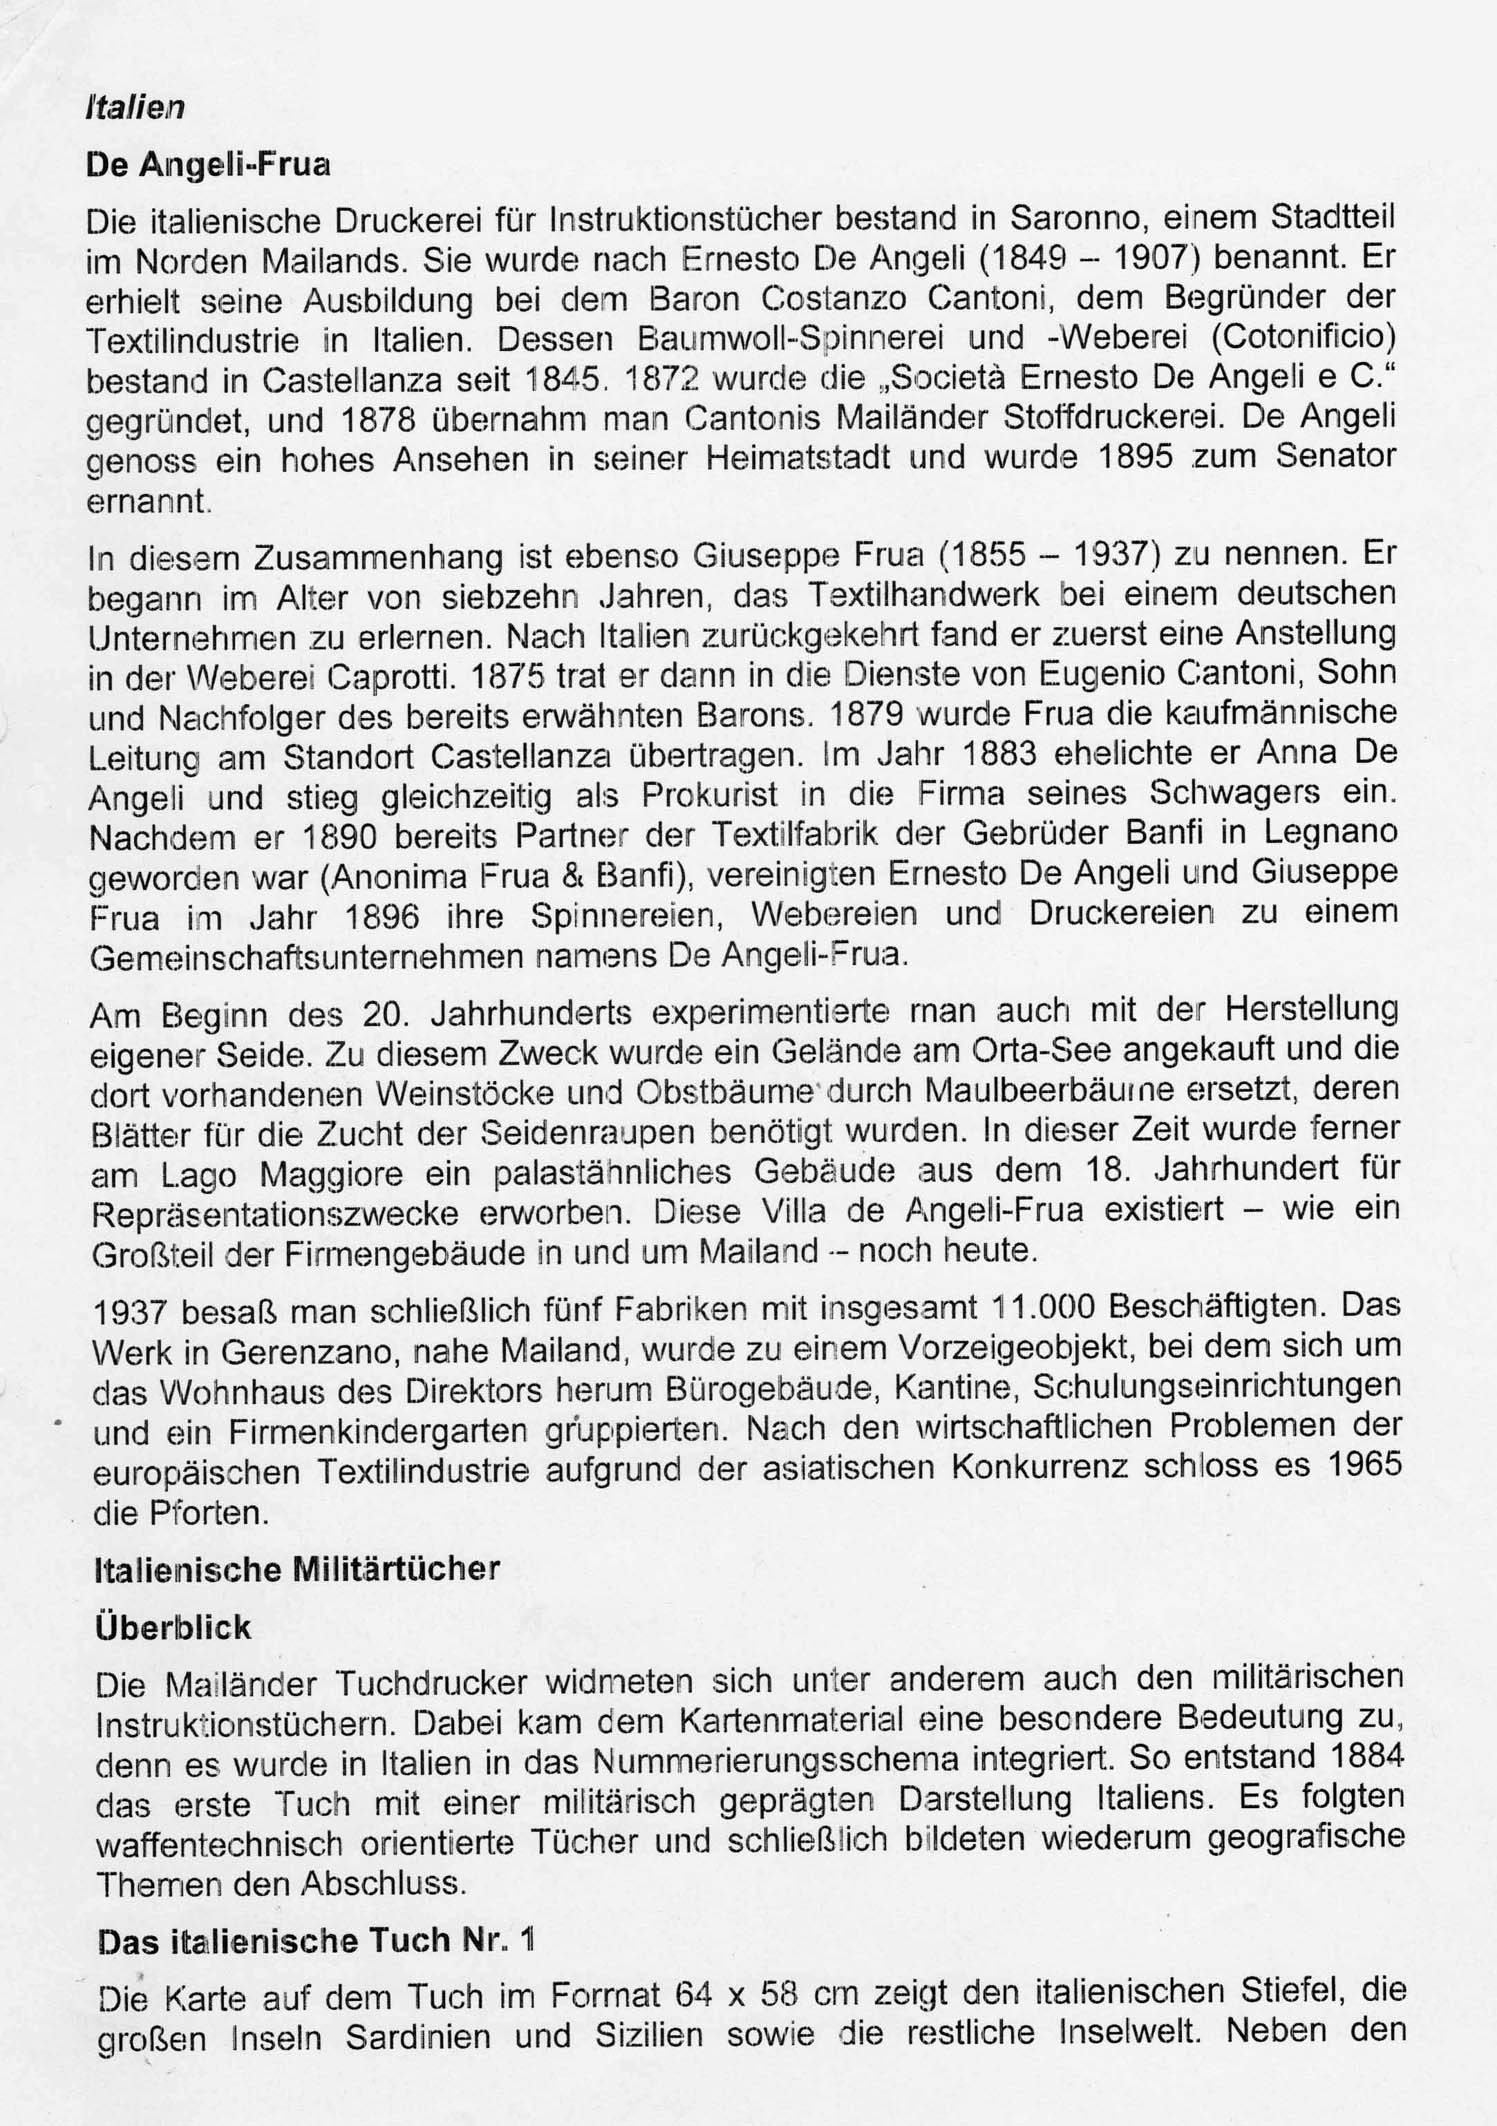
\includegraphics[width=\textwidth]{deangelifrua.jpg}
	\caption{}
	\label{fig:deangelifrua}
\end{figure}

\newpage

De Angeli-Frua

   La stamperia italiana per fazzoletti d'istruzione era a Saronno, una cittadina a nord di Milano. Era così chiamata dal nome di Ernesto De Angeli (1849-1907). Egli aveva ricevuto la sua formazione dal barone Costanzo Cantoni, il fondatore dell'industria tessile in Italia. La sua filanda e cotonificio era a Castellanza dal 1845. Nel 1872 fu fondata la "Società Ernesto De Angeli \& C." e nel 1878 si aprì la stamperia milanese di Cantoni. De Angeli raggiunse una grande reputazione e nel 1895 fu nominato Senatore.
   In questo contesto si deve citare anche Giuseppe Frua (1855-1937). Iniziò diciassettenne ad imparare la tessitura in un'impresa tedesca. Tornato in Italia trovò un primo impiego nel Cotonificio Caprotti. Nel 1875 entrò nella ditta di Eugenio Cantoni, figlio e successore del già menzionato barone. Nel 1879 Frua assunse la direzione commerciale della sede di Castellanza. Nel 1883 sposò Anna De Angeli e divenne Procuratore della ditta del cognato. Poi nel 1890 divenne socio della fabbrica tessile dei fratelli Banfi a Legnano (Anonima Frua \& Banfi), nel 1896 Ernesto De Angeli e Giuseppe Frua unirono le loro filature, cotonifici e stamperie in una società denominata De Angeli-Frua.
   All'inizio del XX secolo sperimentò anche la fabbricazione della seta. A questo fine fu acquistato un terreno sul lago d'Orta e furono sostituiti i vigneti ed i frutteti con piante di gelso, delle cui foglie vi era necessità per l'allevamento dei bachi da seta. Inoltre, in quel tempo fu acquistato sul Lago Maggiore un palazzetto del 18° secolo a scopo di rappresentanza. Questa villa De Angeli Frua esistette, come parte della ditta a Milano, fino ad oggi.
   Nel 1937 si contavano 5 fabbriche con 11000 addetti. Lo stabilimento di Gerenzano, vicino a Milano, fu un fiore all'occhiello, nel quale intorno all'abitazione del Direttore stavano edifici per uffici, mensa, scolastici ed un asilo aziendale. In seguito ai problemi economici dell'industria tessile europea nei confronti della concorrenza asiatica, chiuse nel 1965.


I fazzoletti militari Itaiani

Sguardo d'insieme
  
 Lo stampatore di fazzoletti milanese si dedicò anche ai fazzoletti d'istruzione militare. Il materiale cartografico è particolarmente importante, perché fu inserito in Italia in uno schema numerico. Così nel 1884 nacque in Italia il primo fazzoletto ad impronta militare. Seguirono fazzoletti indirizzati alla tecnica militare ed infine con temi geografici.

\newpage

Il fazzoletto italiano n°1 (vedi pag. 40)
  
 La mappa riprodotta sul fazzoletto nel formato 64 x 58 cm mostra lo stivale italiano, le grandi isole di Sardegna e Sicilia e il resto dell'arcipelago.
 
\begin{figure}[h]
	\centering
		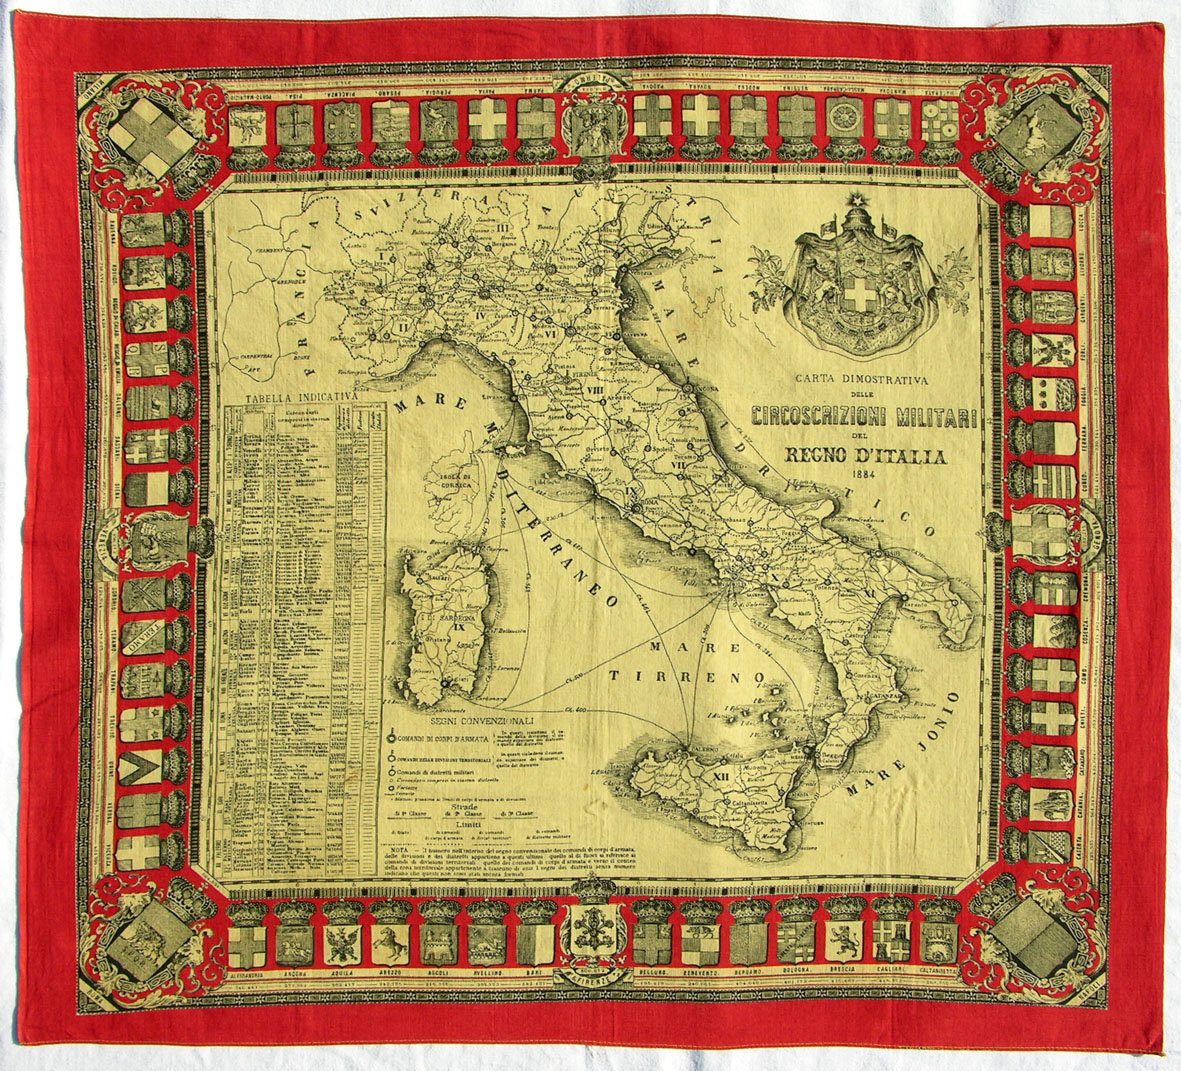
\includegraphics[width=\textwidth]{fazzoletto1_cartaitalia.jpg}
	\caption{Carta d’Italia 1884 Fazzoletto militare italiano n°1 Stamperia De Angeli – Milano}
	\label{fig:fazzoletto1_cartaitalia}
\end{figure}

\newpage

\begin{figure}[h]
	\centering
		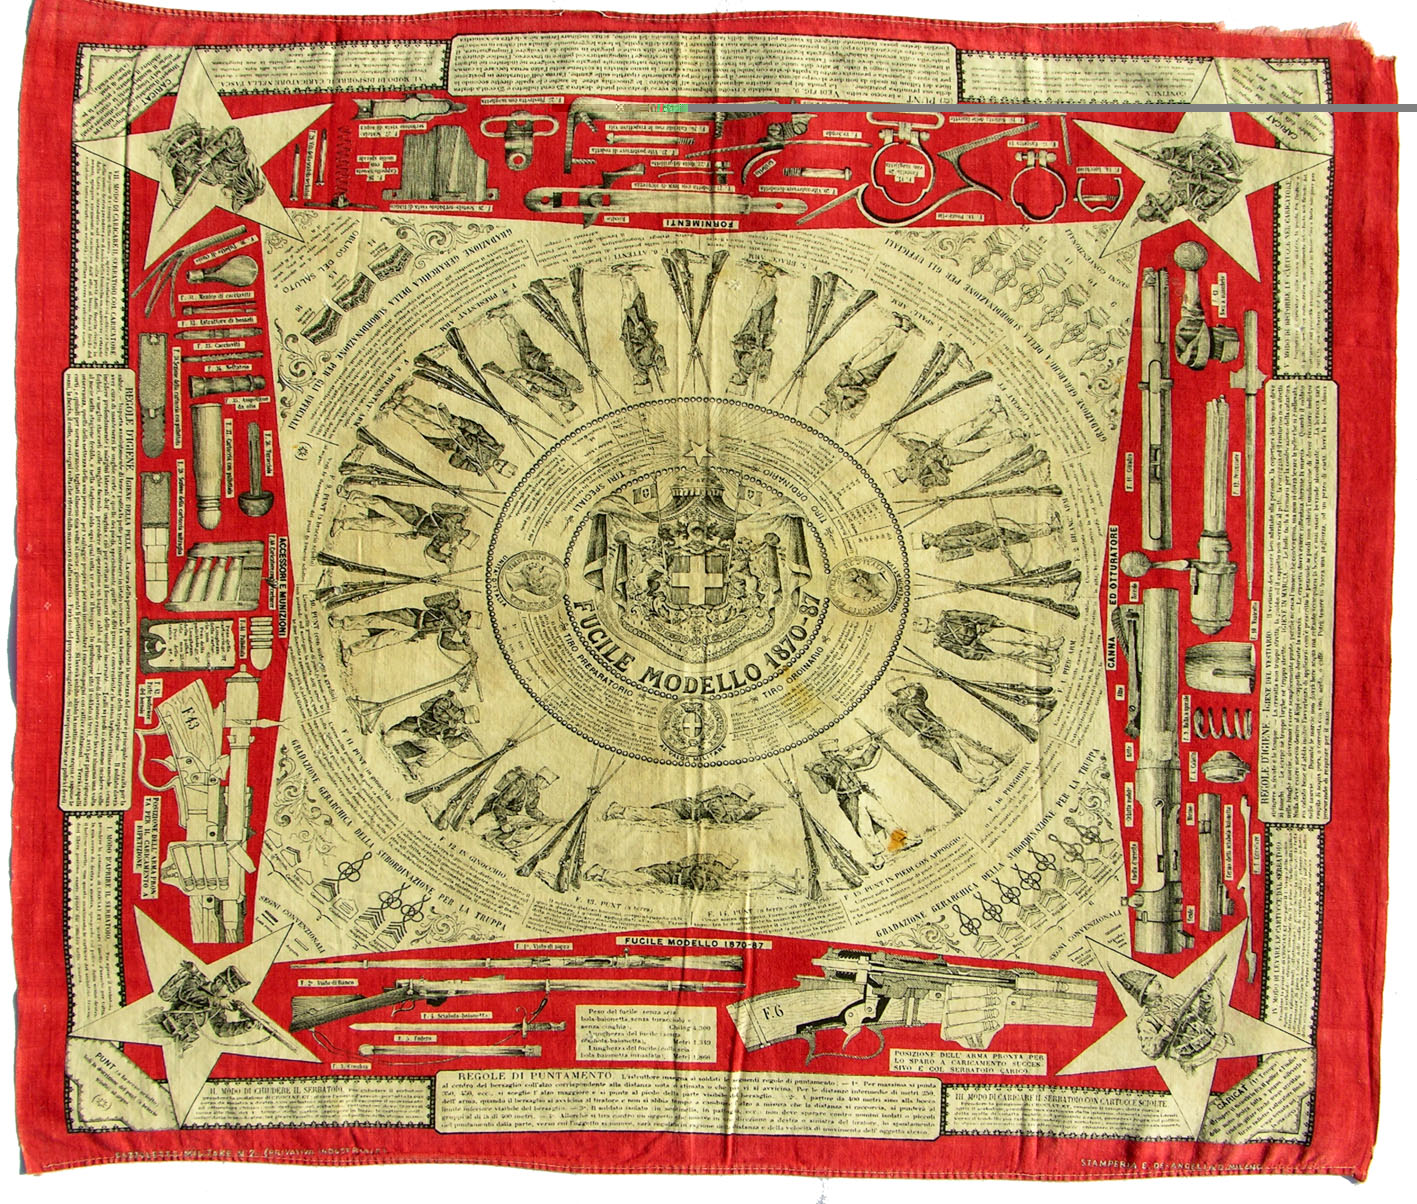
\includegraphics[width=\textwidth]{fazzoletto2.jpg}
	\caption{Fazzoletto militare italiano n°2 Stamperia De Angeli – Milano}
	\label{fig:fazzoletto2}
\end{figure}

\newpage

\begin{figure}[h]
	\centering
		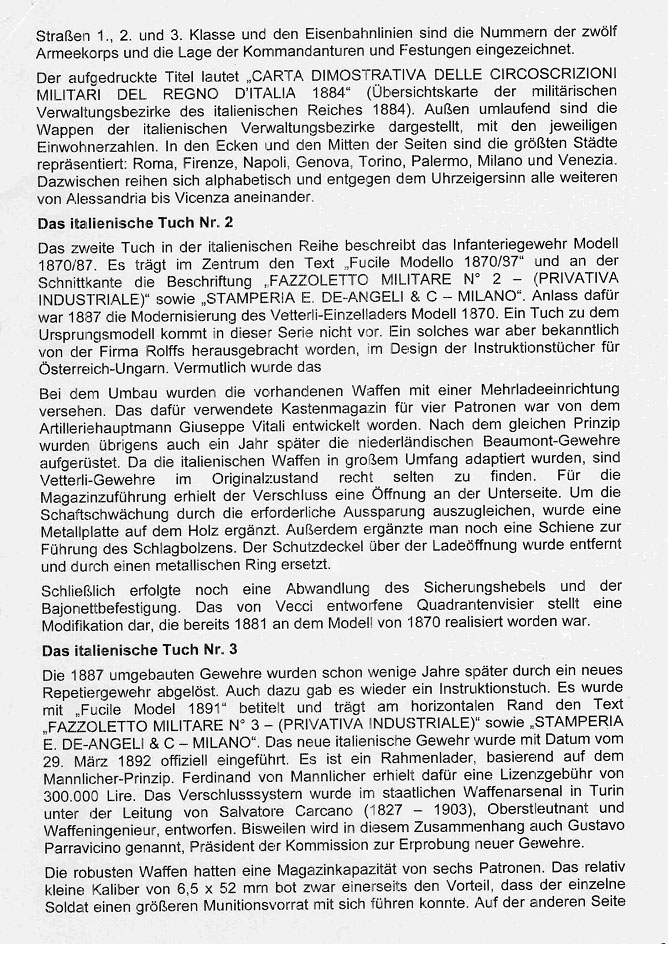
\includegraphics[width=\textwidth]{deangelifrua_2.jpg}
	\caption{}
	\label{fig:deangelifrua_2}
\end{figure}

\newpage

Oltre alle strade di 1a, 2a e 3a classe e le linee ferroviarie, compaiono i numeri dei dodici corpi d'armata dell'esercito e la posizione dei posti di comando e delle fortificazioni.
   II titolo stampato recita "CARTA DIMOSTRATIVA DELLE CIRCOSCRIZIONI MILITARI DEL REGNO D'ITALIA 1884" (mappa panoramica delle circoscrizioni militari del Regno d'Italia nel 1884). Sulla circonferenza esterna sono rappresentati gli stemmi dei distretti italiani, con i dati della popolazione. Negli angoli e al centro dei lati sono rappresentate le maggiori città: Roma, Firenze, Napoli, Genova, Torino, Palermo, Milano e Venezia. Esse sono allineate in ordine alfabetico e in senso antiorario da Alessandria a Vicenza.

Il fazzoletto italiano n°2 (vedi pag. 41)
  
 II secondo fazzoletto della serie italiana descrive il modello del fucile 1870/87 Nel centro figura il testo "Fucile Modello 1870/87" e sul bordo “FAZZOLETTO MILITARE N° 2 - (PRIVATIVA INDUSTRIALE)” e "STAMPERIA E. DE ANGELI \& C - MILANO". L'occasione fu quella, nel 1887, dell'ammodernamento del modello Vetterli del 1870. Un fazzoletto relativo a questo modello non è disponibile. Esso era stato prodotto dalla ditta Rolffs,(vedi pag. 44) come modello dei fazzoletti di istruzioni per l'Austria-Ungheria. 
   All'atto del miglioramento, le armi esistenti sono state dotate di un caricatore multiplo. Il caricatore utilizzato per quattro cartucce era stato sviluppato dal capitano d'artiglieria Giuseppe Vitali. Seguendo lo stesso principio un anno dopo, furono aggiornate le armi olandesi Beaumont. Dal momento che le armi italiane sono state adattate in larga misura, fucili Vetterli in condizioni originali sono abbastanza rari da trovare. II caricatore per l'alimentazione è dotato di un'apertura sul fondo. Per compensare l'indebolimento del fusto, una lastra di metallo è stata aggiunta al legno. Inoltre, si aggiunse una guida per il percussore. Il coperchio di protezione del carico superiore è stato rimosso e sostituito da un anello metallico. 
   Infine, c'è stata una variazione della sicura e della baionetta. Il mirino a quadrante elaborato da Vecci rappresenta una modifica che è stata attuata nel 1881 sul modello del 1870.

Il fazzoletto italiano N°3 (vedi pag. 45)
  
 I fucili 1887 sono stati sostituiti pochi anni dopo con un nuovo fucile a ripetizione. Inoltre, ci fu ancora una volta un fazzoletto di istruzioni. E' intitolato "Fucile Modello 1891” e porta sul bordo orizzontale il testo "FAZZOLETTO MILITARE n ° 3 - (PRIVATIVA INDUSTRIALE)" e “STAMPERIA E. DE ANGELI \& C – MILANO”. 
   Il nuovo fucile italiano è stato introdotto in data 29 Marzo 1892. Si tratta di un caricatore basato sul principio Mannlicher. Ferdinand von Mannlicher si era aggiudicata una fornitura di 300.000 lire. L'otturatore era stato progettato nell'arsenale di Torino da Salvatore Carcano (1827-1903), tenente colonnello e costruttore di armi. A volte viene richiamato in questo contesto, anche il nome di Gustavo Parravicino, Presidente della Commissione per la sperimentazione della nuova arma.
   
\newpage

La robusta arma aveva una capacità di sei pallottole. Il calibro relativamente piccolo di 6,5 x 52 mm, da un lato, ha offerto il vantaggio a ciascun soldato di poter portare con sé una maggiore quantità di munizioni.

\begin{figure}[h]
	\centering
		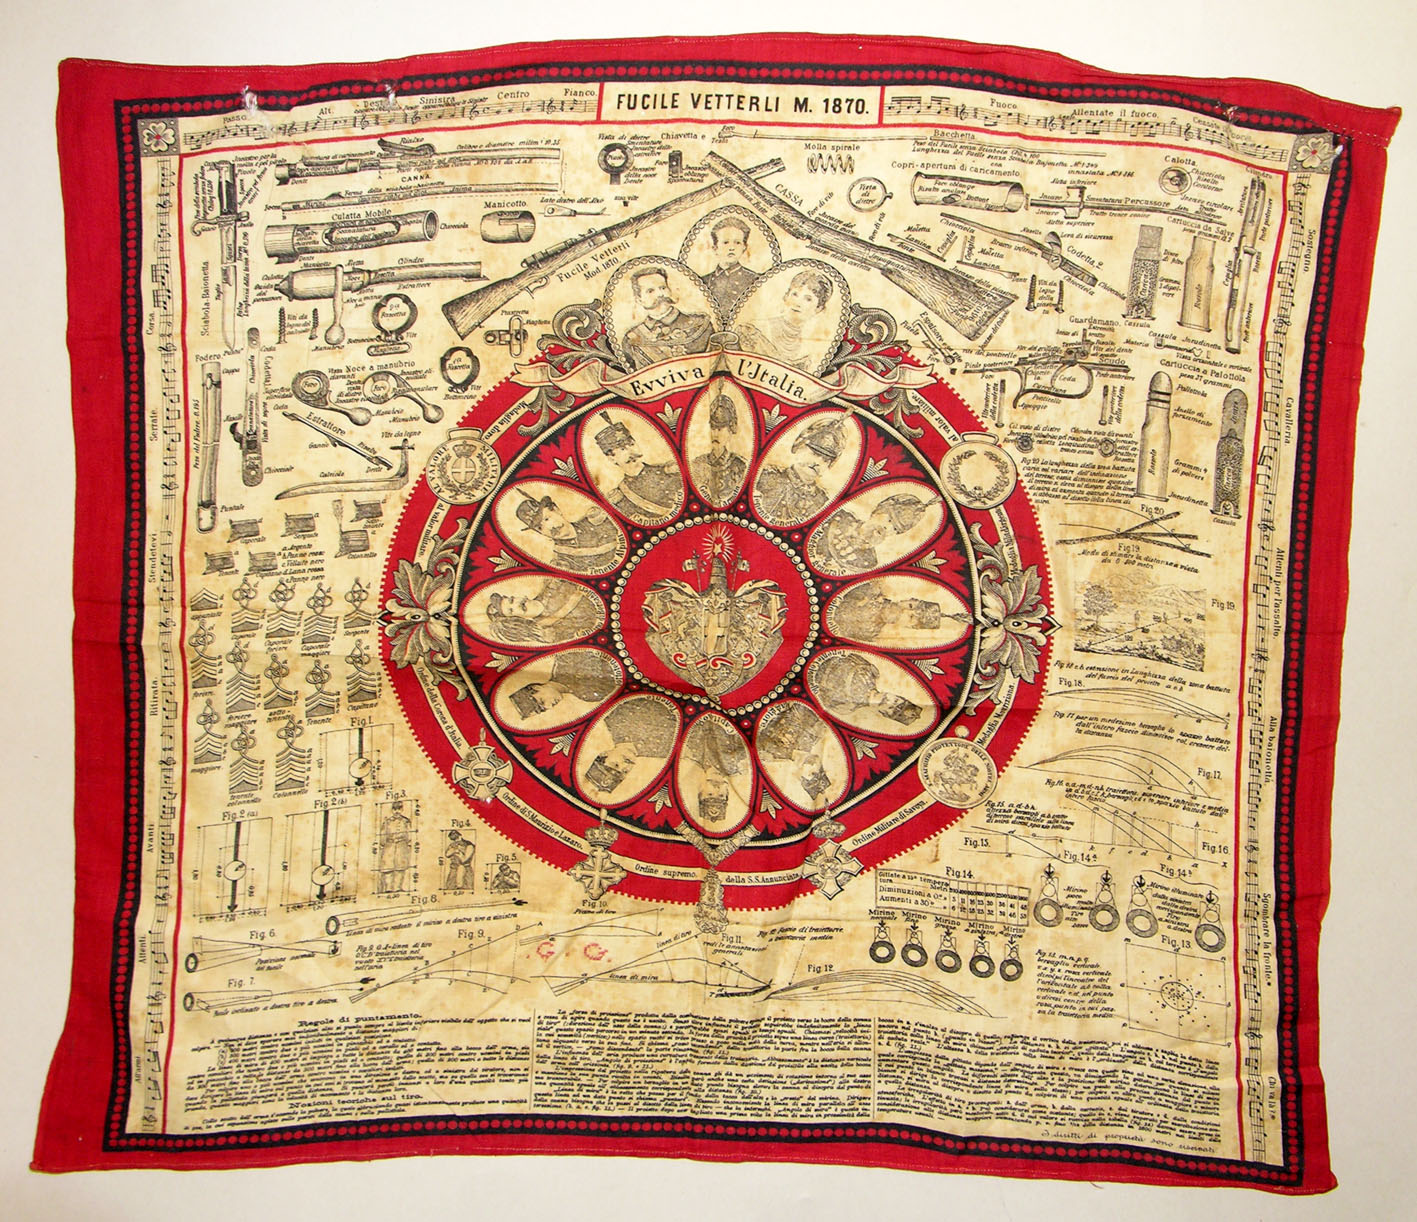
\includegraphics[width=\textwidth]{fazzoletto2A_rollfs.jpg}
	\caption{Fazzoletto militare n° 2A Rolffs \& Co.}
	\label{fig:fazzoletto2A_rollfs}
\end{figure}

\newpage

\begin{figure}[h]
	\centering
		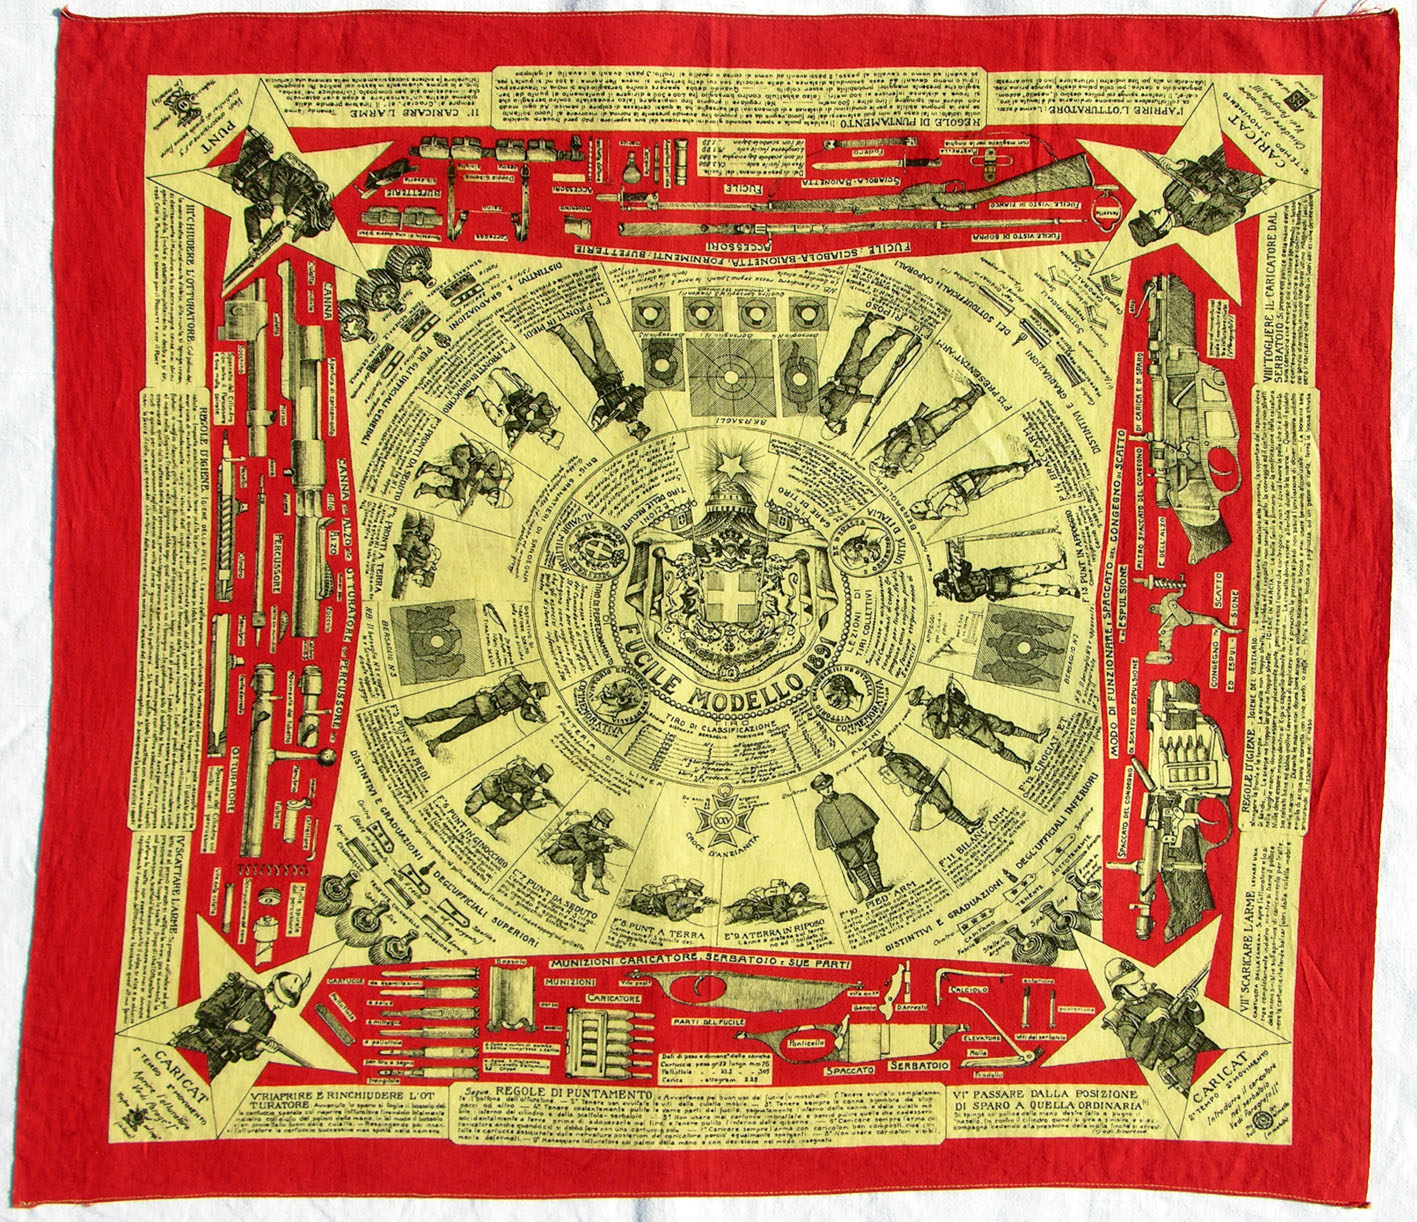
\includegraphics[width=\textwidth]{fazzoletto3.jpg}
	\caption{Fazzoletto militare italiano n°3. Stamperia De Angeli – Milano}
	\label{fig:fazzoletto3}
\end{figure}

\newpage

\begin{figure}[h]
	\centering
		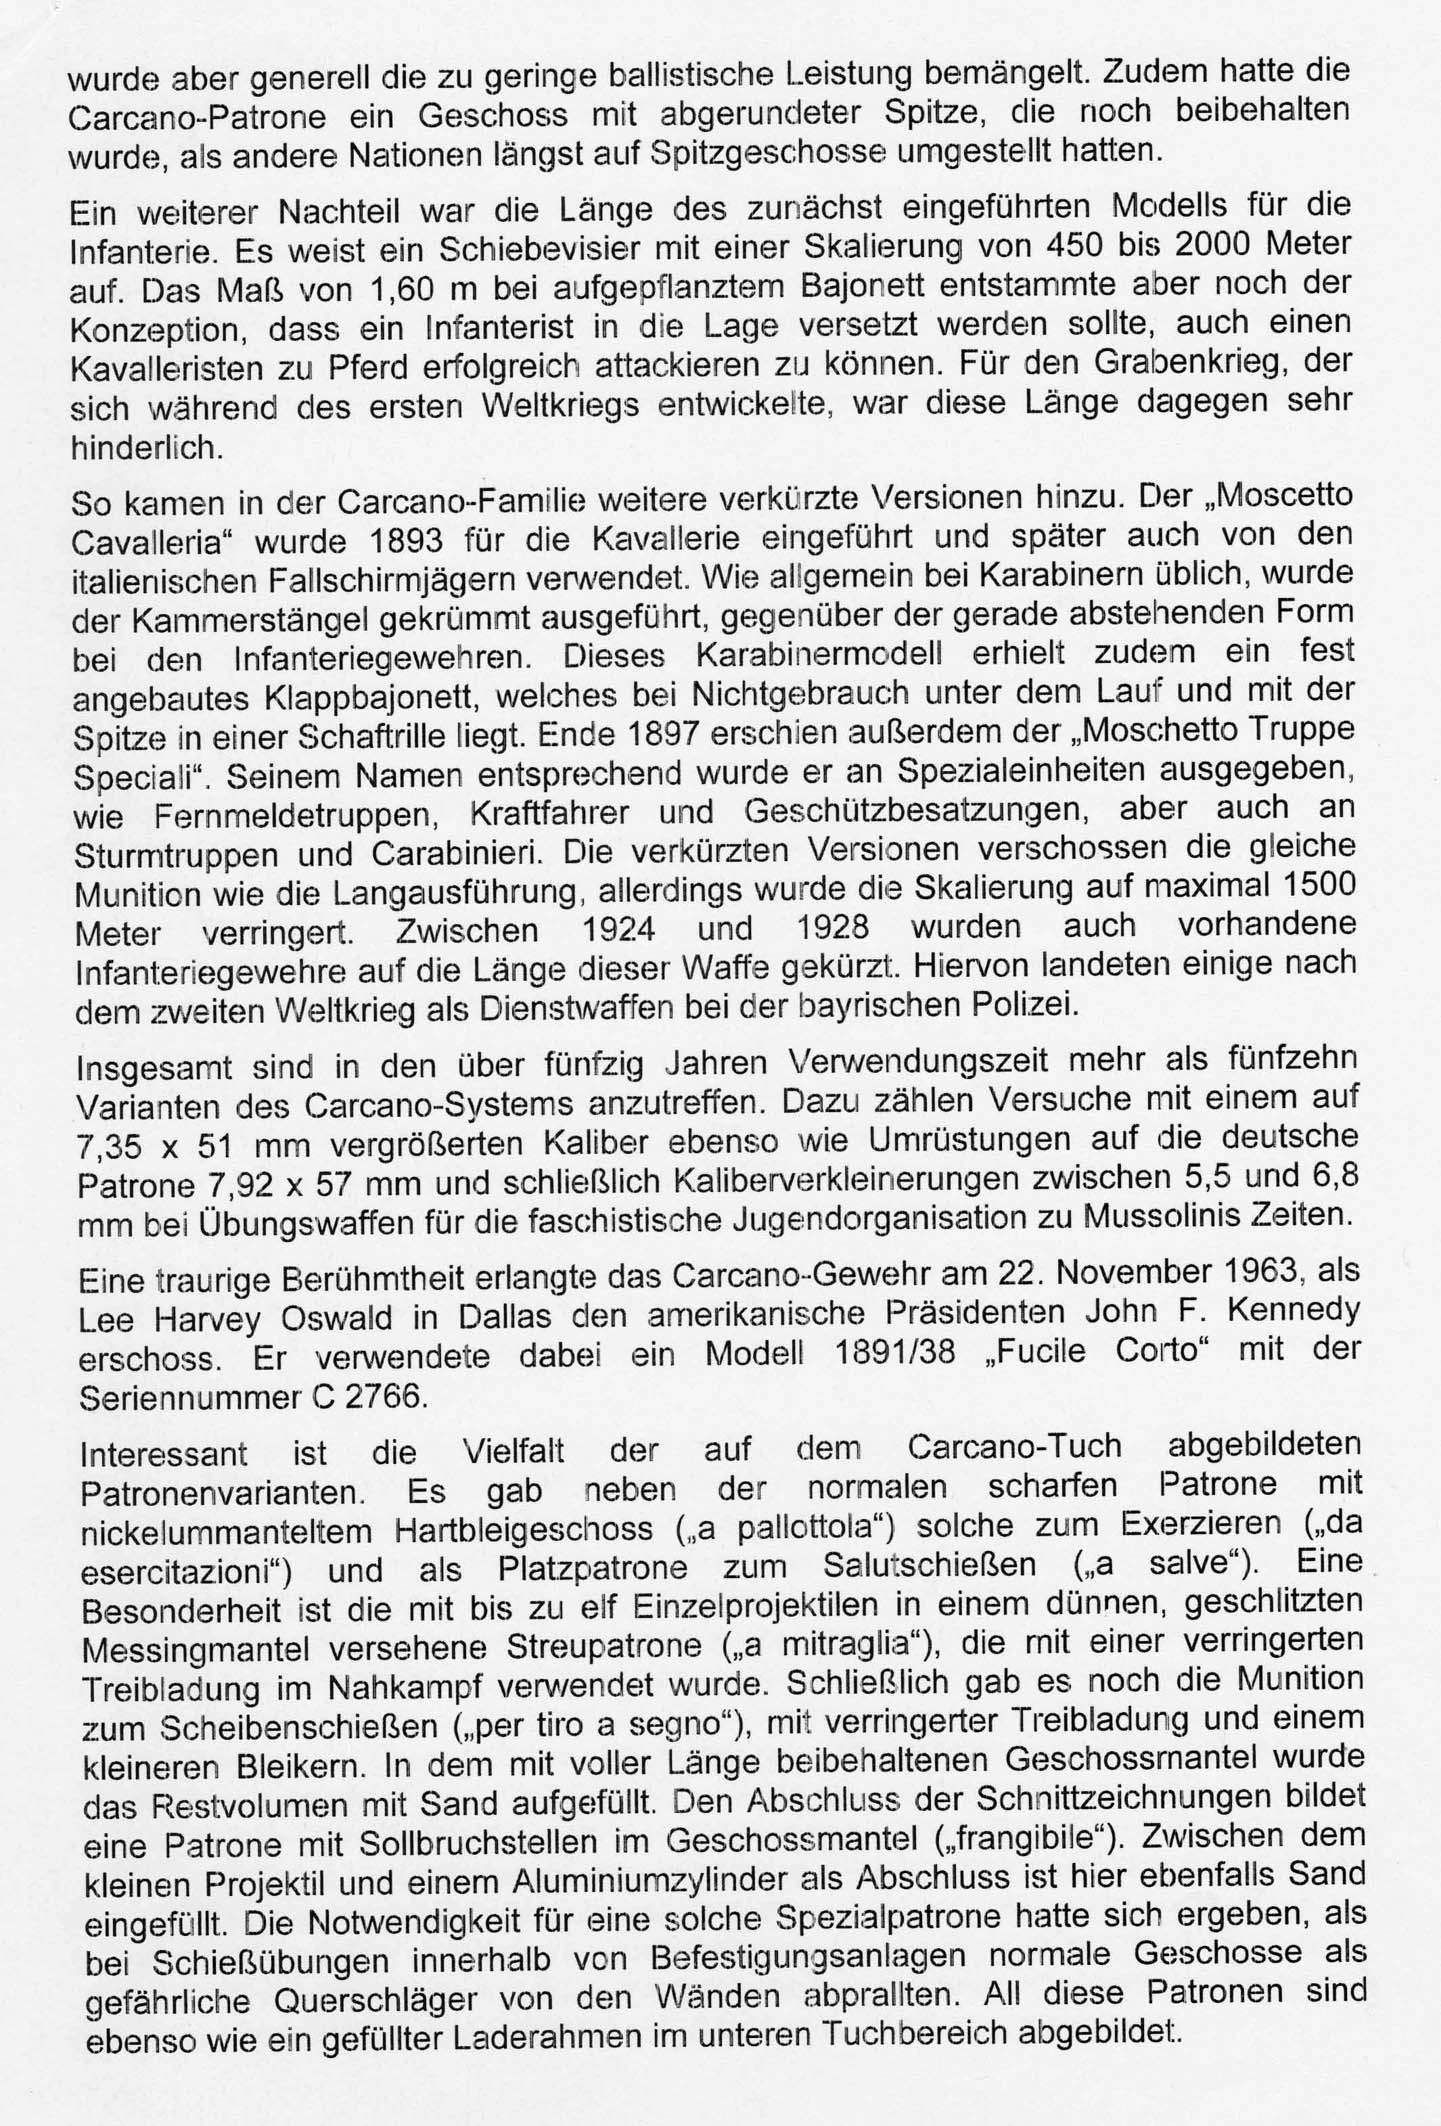
\includegraphics[width=\textwidth]{deangelifrua_3.jpg}
	\caption{}
	\label{fig:deangelifrua_3}
\end{figure}

\newpage

D'altra parte, sono state generalmente criticate le inadeguate prestazioni balistiche. Inoltre, la cartuccia Carcano che era ancora mantenuta, era un proiettile con punta arrotondata, mentre in altre nazioni da tempo si erano convertiti i proiettili. 
   Un altro svantaggio è la lunghezza del primo modello introdotto per la fanteria. Ha un mirino con una scala mobile 450-2000 metri. La lunghezza di 1,60 m con baionetta innestata, riflette ancora il concetto che un soldato dovrebbe essere in grado di attaccare anche un cavalliere per avere successo. Per la guerra di trincea, che si è sviluppata durante la Prima Guerra Mondiale, ciò è stato di molto ostacolo.
   Così si aggiunsero alla famiglia Carcano versioni ridotte. Il "Moschetto Cavalleria" è stato introdotto nel 1893 per la cavalleria e poi utilizzato dai paracadutisti italiani. Questo modello è stato anche dotato di una baionetta pieghevole, che si trova sotto la canna quando non in uso e con la punta in una scanalatura. Alla fine del 1897 apparve anche il "Moschetto Truppe Speciali". Come dice il suo nome è stato prodotto per unità speciali, come le truppe di telecomunicazioni, cannonieri e piloti, ma anche le truppe d'assalto ed i carabinieri. Le versioni accorciate sparavano le munizioni stesse di quelle lunghe, tuttavia, la portata era ridotta fino a un massimo di 1500 metri. Tra il 1924 e il 1928 i fucili di fanteria esistenti sono stati accorciati alla lunghezza di quest'arma. Di questi, alcuni finirono dopo la Seconda Guerra Mondiale usati come arma di servizio dalla polizia bavarese.
   Nel complesso, in un periodo superiore ai 50 anni furono usate più di quindici varietà di armi con sistema Carcano. Queste includono calibri allargati a 7,35 mm x 51, nonché cartucce tedesche calibro 7,92 x 57 mm e infine la riduzione dal 5,5-6,8 mm per l'organizzazione giovanile fascista al tempo di Mussolini.
   Una notorietà fu acquisita dal fucile Carcano il 22 Novembre 1963, quando Lee Harvey Oswald, a Dallas, uccise il presidente americano John F. Kennedy. Usò un modello 1891/38 "Fucile Corto" con il numero di serie C 2766.
   Interessante è la diversità delle cartucce raffigurate sul fazzoletto-Carcano. Ci sono, oltre alla normale cartuccia con copertura di nickel ("a pallottola") quelle per esercitazione ("da esercitazioni") ed una cartuccia a salve ("a salve"). Una caratteristica particolare è il massimo di undici proiettili singoli in un sottile involucro di ottone ("a mitraglia"), che è stato utilizzato con una carica propellente ridotta nelle mischie. Infine c'erano le munizioni per il tiro al bersaglio ("per Tiro a Segno"), con carica propellente ridotta e un nucleo in piombo più piccolo. Per mantenere la lunghezza completa il volume rimanente era riempito con sabbia. La conclusione dei disegni in sezione mostra una cartuccia con punti di rottura ("Frangibile"). Fra il proiettile e un piccolo cilindro di alluminio il terminale è pieno di sabbia. La necessità di tale una speciale cartuccia si era evidenziata, dal momento che nel tiro al bersaglio con normali proiettili essi rimbalzavano pericolosamente colpendo le pareti. Queste cartucce sono mostrate nell'area inferiore del fazzoletto.
Sui fazzoletti italiani si possono anche trovare le immagini e le spiegazioni delle varie formazioni di fanteria.

\newpage

\begin{figure}[h]
	\centering
		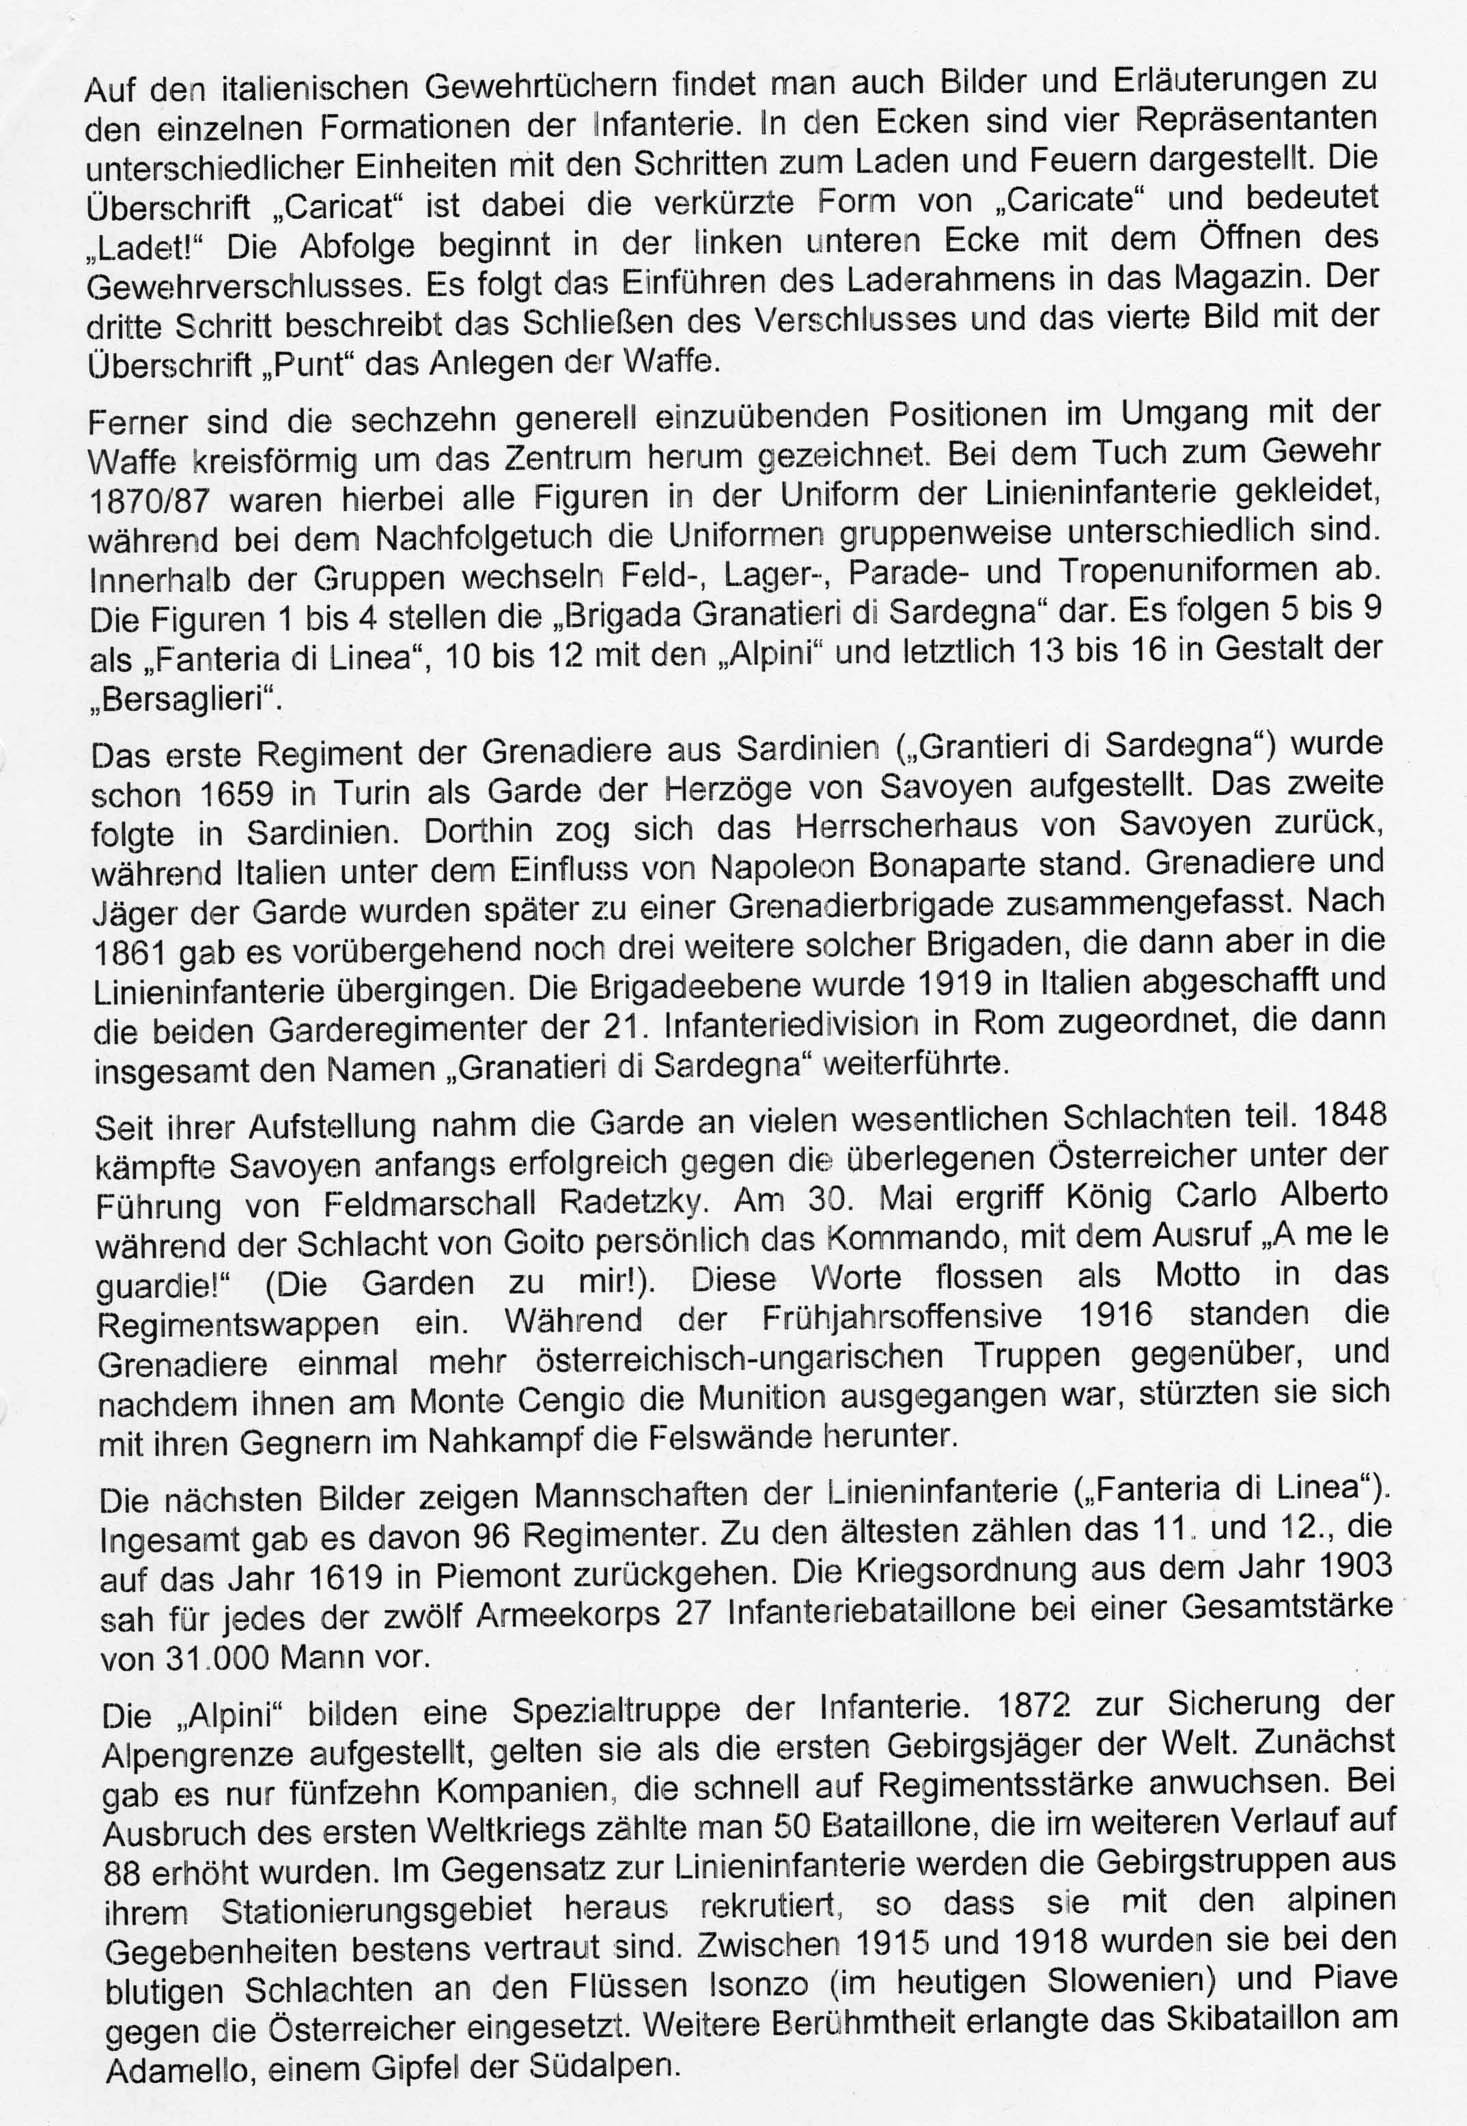
\includegraphics[width=\textwidth]{deangelifrua_4.jpg}
	\caption{}
	\label{fig:deangelifrua_4}
\end{figure}

\newpage

Negli angoli stanno quattro rappresentanti di diverse unità che mostrano i passaggi per il caricamento ed il fuoco. La scritta "caricat" è la forma abbreviata di "caricate" e significa "Carica!" La sequenza inizia nell'angolo in basso a sinistra con l'apertura della caricatore. Ne consegue l'introduzione dei proiettili nel caricatore. Il terzo passo descrive la chiusura e la quarta immagine con la scritta"punt" nella parte superiore il puntamento dell'arma.
   Inoltre, sono illustrate le sedici posizioni generali uso dell'arma in un cerchio intorno al centro. Nel fazzoletto per fucile 1870/87 le figure sono tutte in uniforme della fanteria di linea, mentre nei fazzoletti successivi i gruppi di divise sono diversi. All'interno dei gruppi le uniformi sono da campo, da deposito, da parata e coloniali. Le figure da 1 a 4 rappresentano la "Brigata Granatieri di Sardegna" A seguire da 5 a 9 la "Fanteria di Linea", da 10 a 12 gli "Alpini" e infine da 13 a 16 i "Bersaglieri".
II primo reggimento dei Granatieri di Sardegna  fu istituito nel 1659 a Torino come guardia dei duchi di Savoia. 
   II secondo seguì in Sardegna. Ci si era ritirata la casa regnante dei Savoia, mentre l'Italia era sotto l'influenza di Napoleone Bonaparte. I Granatieri della Guardia e i Cacciatori sono stati successivamente raccolti in una brigata. Dopo il 1861 ci furono altre tre brigate, ma poi confluirono nella fanteria di linea. La brigata è stata abolita nel 1919 in Italia e i due reggimenti Guardie della 21 Divisione di fanteria, furono assegnati a Roma, che poi hanno portato il nome di "Granatieri di Sardegna".
   Fin dalla sua costituzione, la Guardia ha partecipato a molte battaglie importanti. Nel 1848 i Savoia inizialmente hanno combattuto con successo contro gli austriaci comandati dal maresciallo Radetzky. Il 30 Maggio re Carlo Albèrto prese il comando personale durante la battaglia di Goito, con l'esclamazione "A me le Guardie!". Queste parole sono state incorporate nel motto del reggimento. Durante l'offensiva di primavera del 1916 i granatieri hanno resistito contro le truppe austro-ungariche, e dopo aver esaurito le munizioni a Monte Cengio, si buttavano giù con i loro nemici in combattimento ravvicinato, dalle pareti di roccia.
   Le immagini successive mostrano di squadre di fanteria di linea ("Fanteria di Linea"). Complessivamente ci sono stati 96 reggimenti. Fra i più antichi sono l'11 e il 12, che risalgono al 1619, in Piemonte. Le ordinanze del 1903 per ciascuno delle dodici corpi di armata dell'esercito, prevedevano 27 battaglioni di fanteria con una forza totale di 31.000 uomini. 
   Gli "Alpini" formano una speciale forza di fanteria. Istituiti nel 1872 per assicurare la frontiera alpina, sono considerati i primi cacciatori di montagna del mondo. Inizialmente c'erano solo quindici compagnie, che crebbero rapidamente alla forza di un reggimento. Allo scoppio della seconda guerra mondiale c'erano 50 battaglioni, che sono stati aumentati a 88. In contrasto con la fanteria di linea, le truppe di fanteria di montagna sono reclutate dalla loro zona di provenienza in modo a essere al corrente delle condizioni alpine. Tra il 1915 e il 1918 furono impiegati in sanguinose battaglie sul fiume Isonzo (oggi in Slovenia) e sul Piave contro gli austriaci. Ebbero fama ulteriormente i battaglioni da sci dell'Adamello, una cima delle Alpi Meridionali.
   
\newpage

\begin{figure}[h]
	\centering
		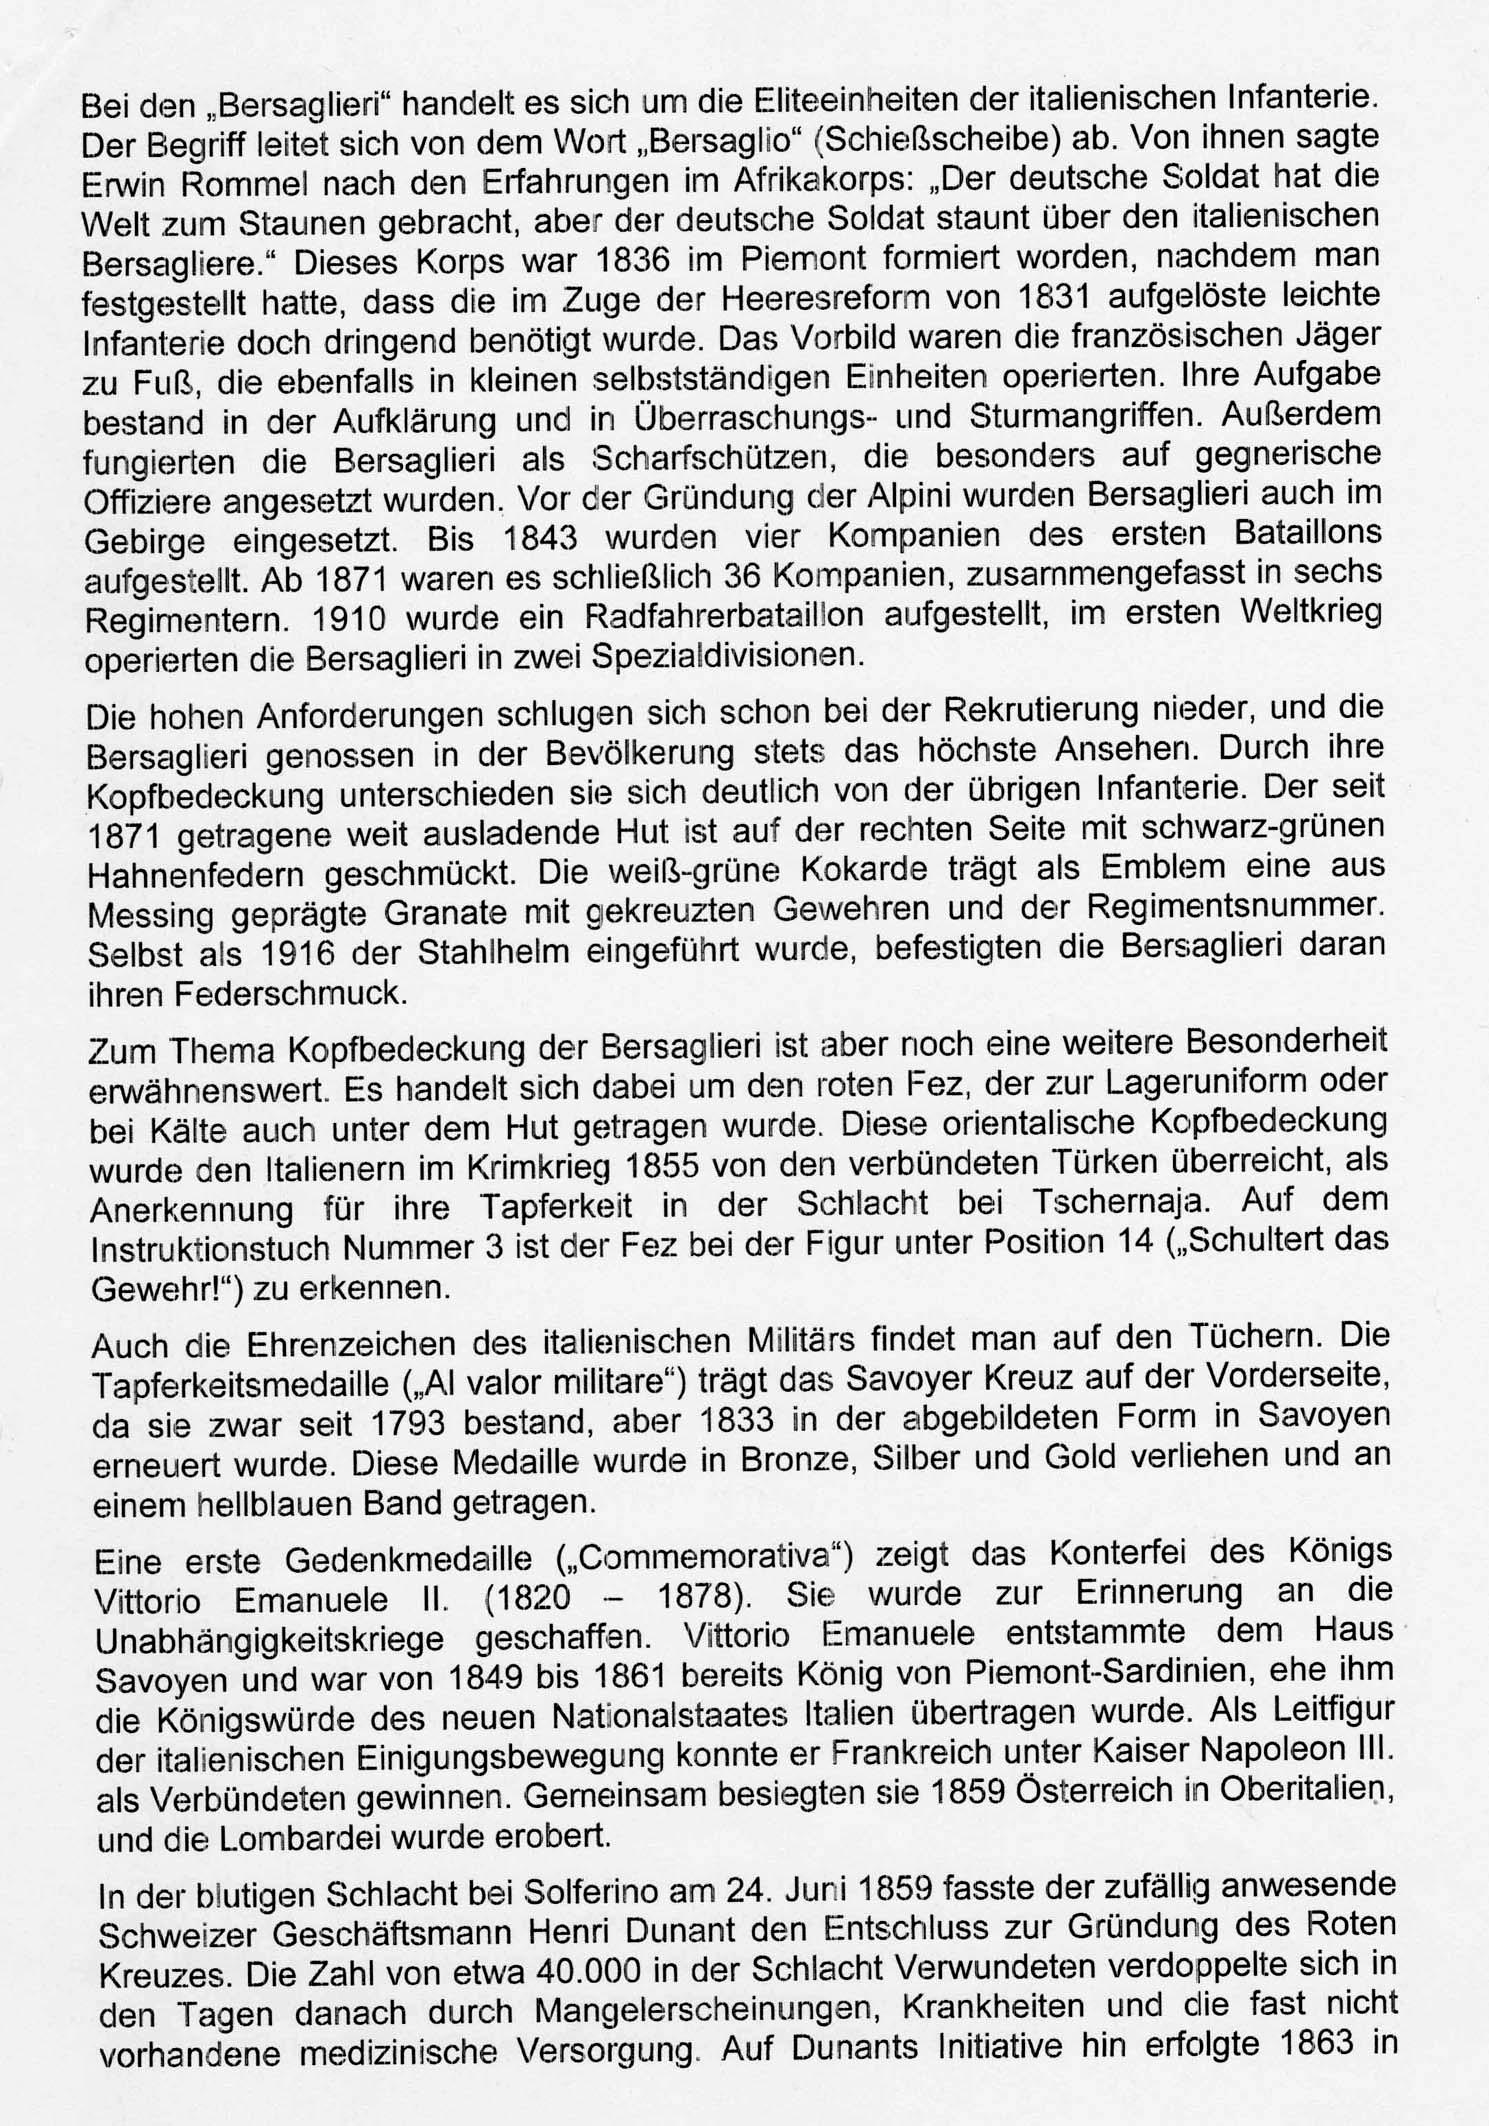
\includegraphics[width=\textwidth]{deangelifrua_5.jpg}
	\caption{}
	\label{fig:deangelifrua_5}
\end{figure}

I "Bersaglieri" sono le unità d'elite della fanteria italiana. Il termine deriva dalla parola "Bersaglio". Erwin Rommel di loro ha detto dopo l'esperienza nell'Afrika korps: "II soldato tedesco è ammirato nel mondo, ma il soldato tedesco ammirò il Bersagliere italiano". Questo corpo si era formato nei 1836 in Piemonte, dopo la riforma dell'esercito del 1831 come di fanteria leggera e rapida. Il modello era il cacciatore francese a piedi, che operava in piccole unità indipendenti. Il loro compito era la perlustrazione, la sorpresa e l'assalto. Operando i bersaglieri come tiratori, che erano particolarmente considerati dagli ufficiali nemici. Prima della fondazione degli Alpini, i Bersaglieri sono stati utilizzati anche in montagna. Fino al 1843, furono schierate quattro compagnie del Primo Battaglione. Dal 1871, ci sono state 36 compagnie raggruppate in sei reggimenti. Nel 1910 è stato allestito un battaglione ciclista. Nella prima guerra mondiale, i bersaglieri operavano in due divisioni speciali.
   I severi requisiti si riflettevano nel reclutamento, e i bersaglieri hanno sempre goduto della massima reputazione da parte della popolazione. Con i loro cappelli, differivano significativamente dal resto della fanteria. Il cappello indossato dal 1871, è decorato sul lato destro con piume di gallo cedrone. La coccarda verde e bianco reca come un distintivo di ottone sbalzato fucili e granate con il numero del reggimento. Anche sull'elmo d'acciaio 1916 i bersaglieri misero le loro piume. A proposito del copricapo dei Bersaglieri vi è ancora da fare un'altra menzione speciale. E 'il fez rosso, che è stato portato nell'uniforme al campo, o quando fa freddo anche sotto il cappello. Questo copricapo orientale fu donato agli italiani nella guerra di Crimea nel 1855, dai turchi alleati, in riconoscimento del loro coraggio nella battaglia di Chernaya. Sul fazzoletto di istruzioni n. 3 il Fez figura al punto 14 ("in spalla il suo fucile!").
   Anche le decorazioni dei militari italiani si trovano sui fazzoletti. La Medaglia ("al valor militare") che porta sulla parte anteriore la croce di Savoia, esisteva sin dal 1793, ma è stata rinnovata nel 1833. Questa medaglia è stata assegnata in bronzo, argento e oro e indossata con un nastro azzurro.
   Una prima medaglia commemorativa  mostra l'immagine di Re Vittorio Emanuele II (1820 - 1878). E 'stata creata per commemorare le guerre di indipendenza. Vittorio Emanuele veniva dalla Casa di Savoia ed era già re di Piemonte-Sardegna dal 1849 al 1861, prima di diventare il Re del nuovo stato nazionale italiano. Come guida del movimento di unificazione italiana, è stato alleato con la Francia sotto l'imperatore Napoleone III. insieme hanno sconfitto l'Austria nel 1859 nel nord Italia, e la Lombardia è stata conquistata.
   
\newpage

Nella sanguinosa battaglia di Solferino, il 24 Giugno 1859 l'imprenditore svizzero Henri Dunant prese la decisione di fondare la Croce Rossa. Il numero di circa 40.000 feriti in battaglia raddoppiò nei giorni seguenti per malattie, e quasi nessuna cura medica a disposizione. Per iniziativa di Dunant a Ginevra nel 1863 fu istituito il "Comitato internazionale di soccorso ai feriti in battaglia".

\begin{figure}[h]
	\centering
		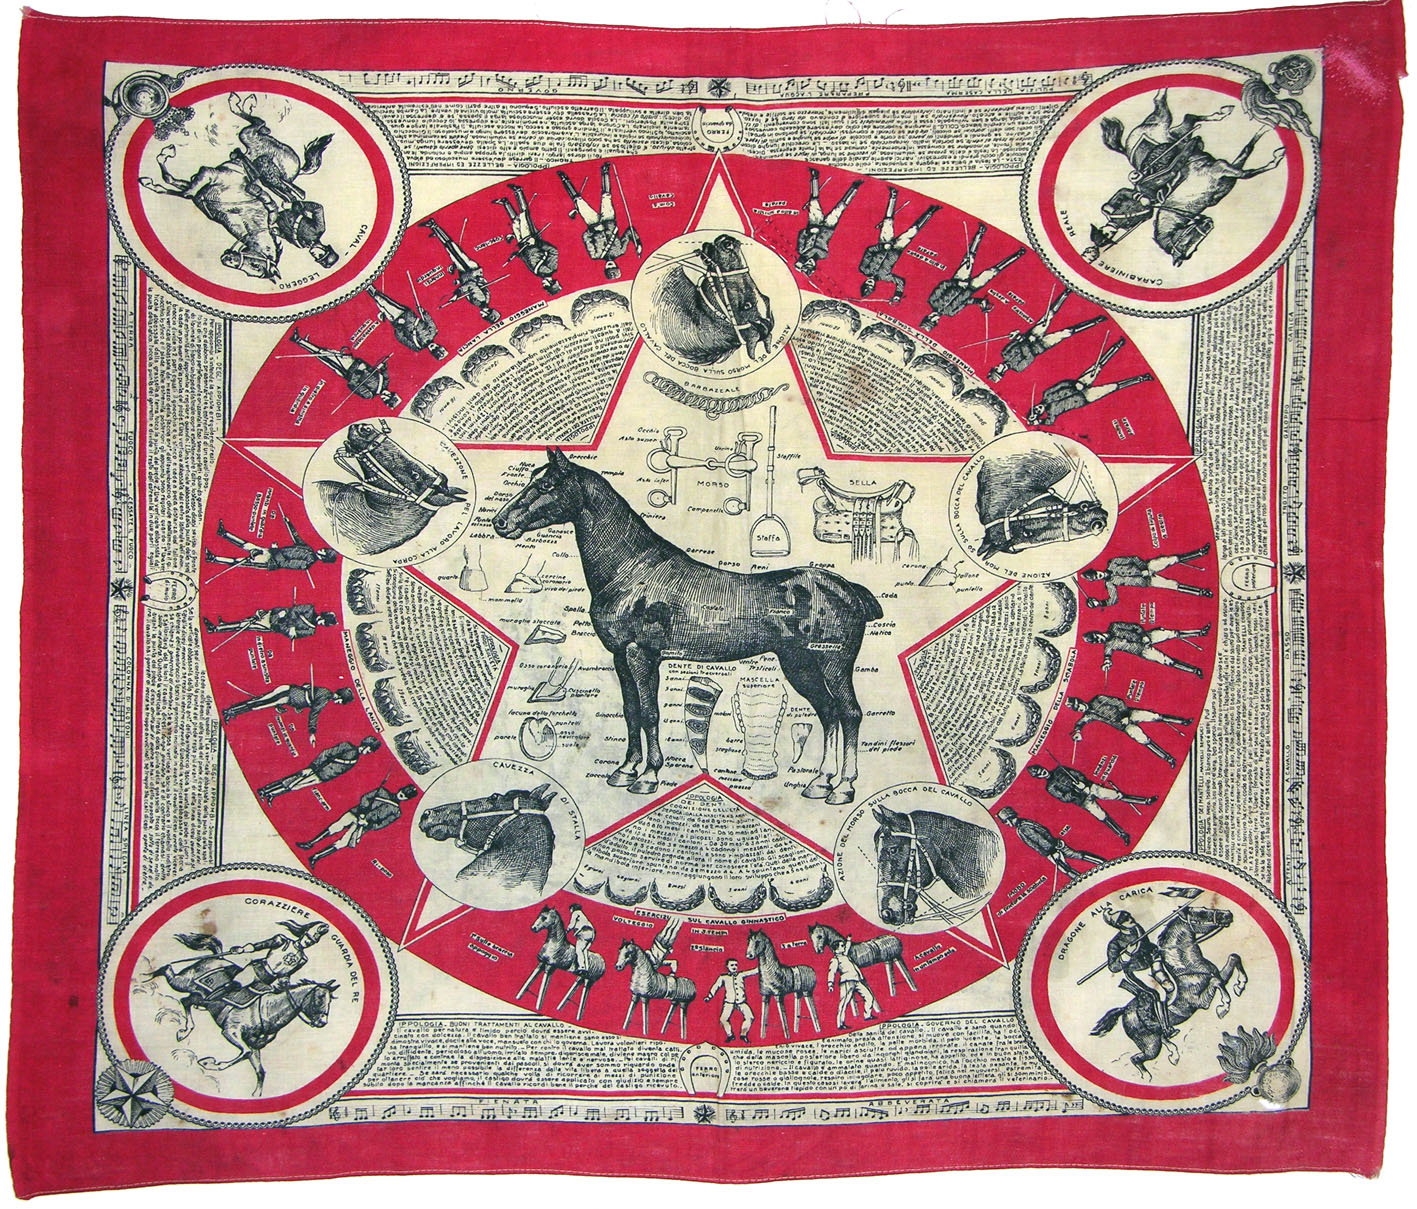
\includegraphics[width=\textwidth]{fazzoletto4_cavalleria.jpg}
	\caption{Fazzoletto militare italiano n°4 per Cavalleria. Stamperia E. De Angeli \&Co. – Milano}
	\label{fig:fazzoletto4_cavalleria}
\end{figure}

\newpage

\begin{figure}[h]
	\centering
		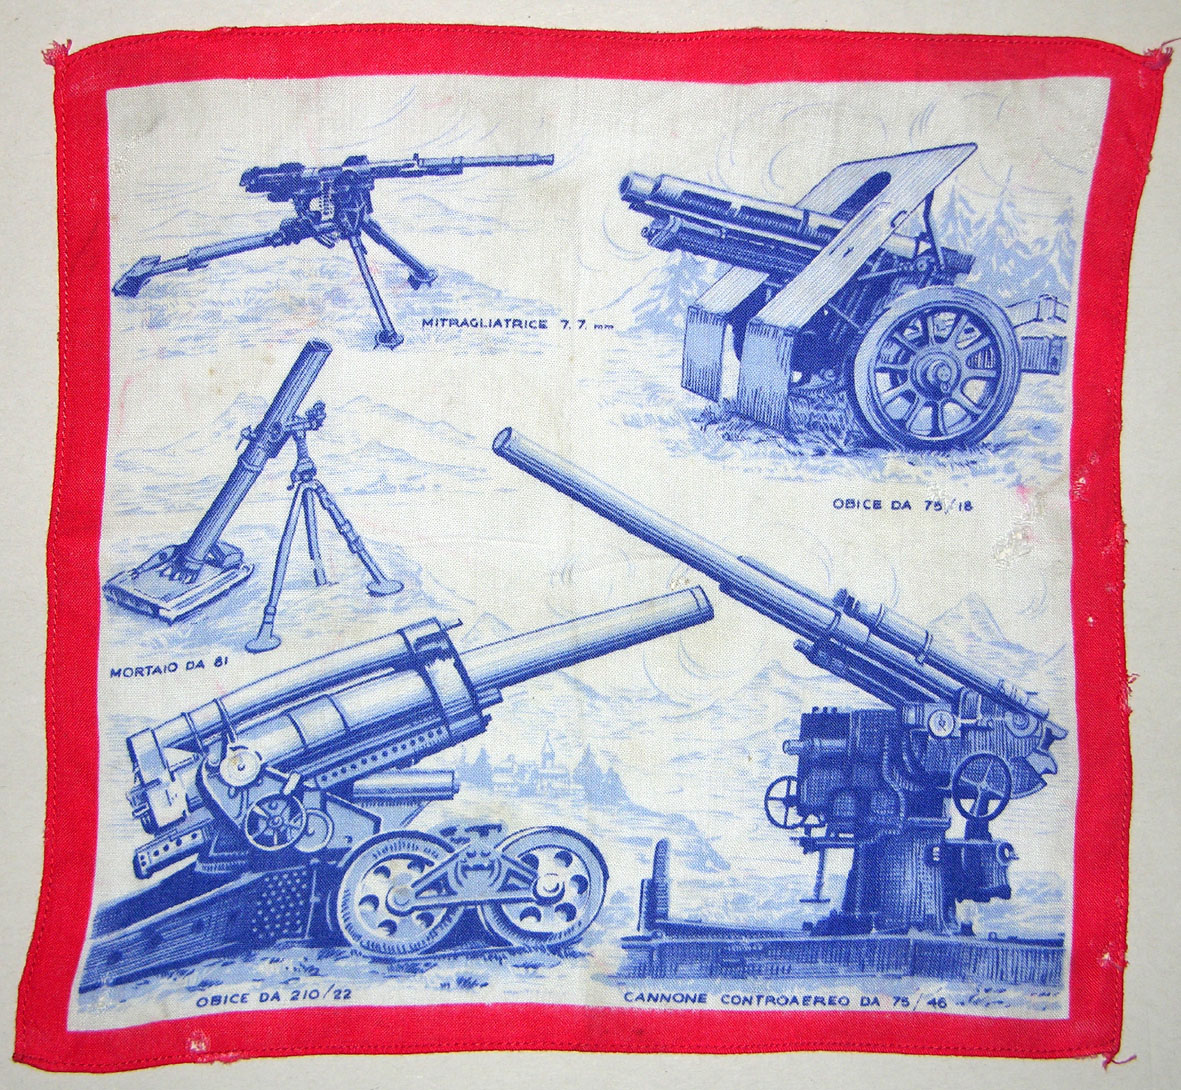
\includegraphics[width=\textwidth]{fazzoletto_armipesanti.jpg}
	\caption{Fazzoletto per armi pesanti}
	\label{fig:fazzoletto_armipesanti}
\end{figure}

\newpage

\begin{figure}[h]
	\centering
		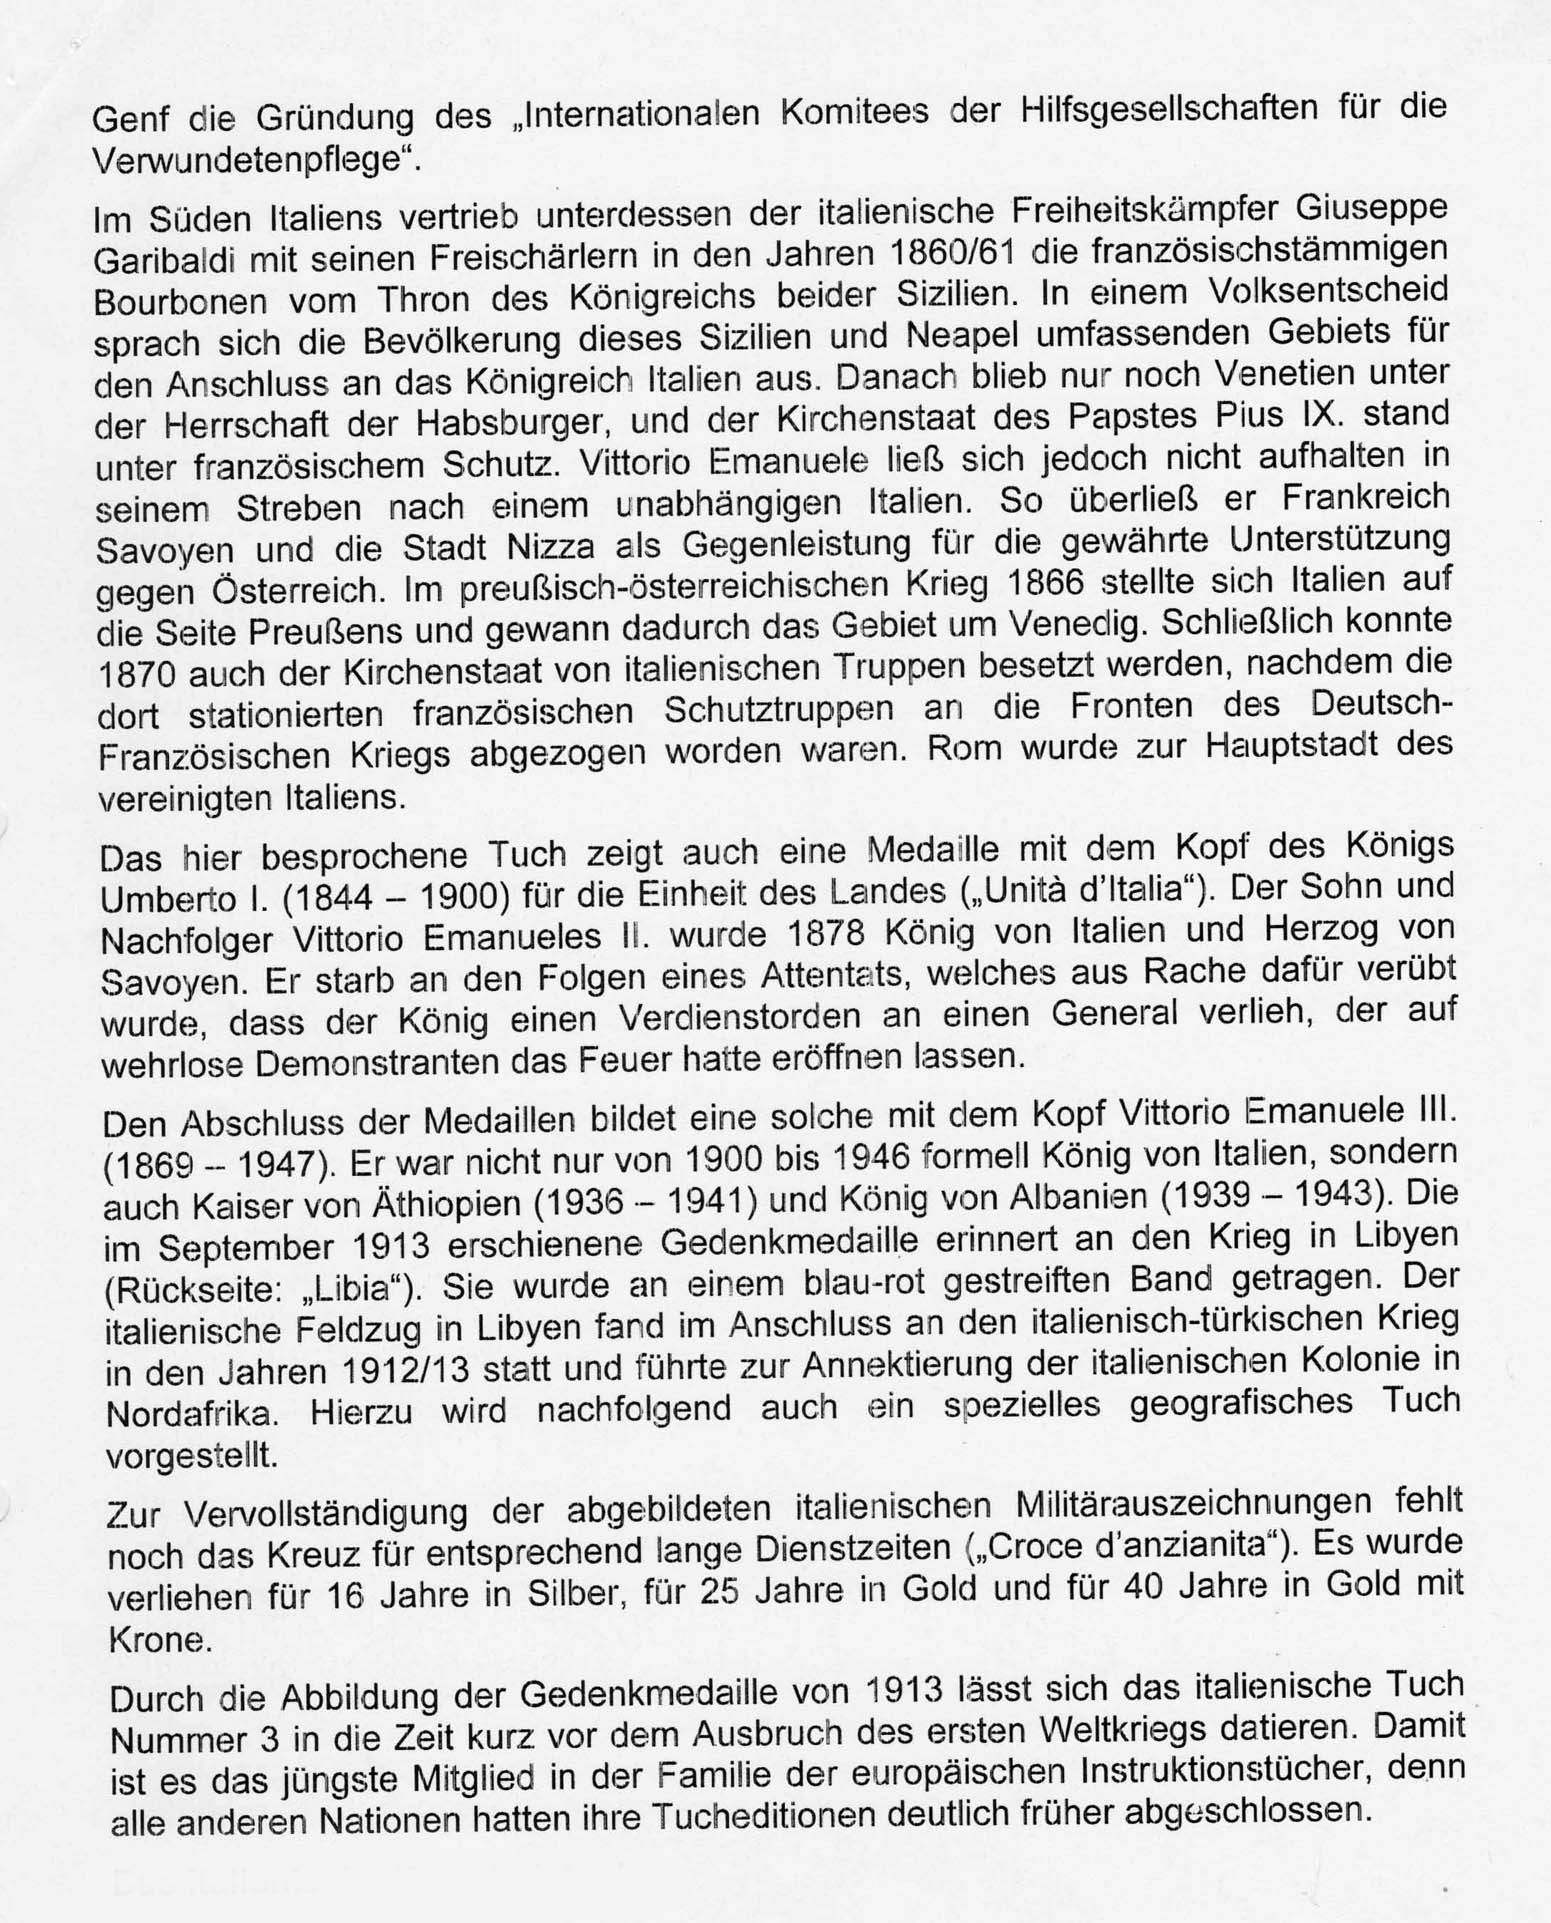
\includegraphics[width=\textwidth]{deangelifrua_6.jpg}
	\caption{}
	\label{fig:deangelifrua_6}
\end{figure}

\newpage

Nel sud Italia, nei frattempo, l'italiano Giuseppe Garibaldi, ha scacciato con i suoi guerriglieri nel 1860/61 i Borboni francesi di nascita dal trono del Regno delle Due Sicilie. in un plebiscito, il popolo di questa vasta area della Sicilia e di Napoli si espresse per l'unione al Regno d'Italia. Da allora in poi solo il Veneto rimase sotto il dominio degli Asburgo, e Io Stato della Chiesa di Papa Pio IX era sotto la protezione francese. Vittorio Emanuele, però, non si fermò nella lotta per l'indipendenza d'Italia. Così lasciò la città di Nizza e la Savoia alla Francia in cambio del sostegno avuto contro l'Austria. Nella guerra austro-prussiana nel 1866 l'Italia si schierò con la Prussia e, quindi, ottenne la zona intorno a Venezia. Infine, nel 1870 anche lo Stato Pontificio è stato occupato dalle truppe italiane, di stanza là dopo che le truppe francesi erano state ritirate per proteggere il fronte della guerra franco-tedesca. Roma divenne capitale dell'Italia unita.
   II fazzoletto riporta anche una medaglia con la effigie del re Umberto I (1844 - 1900) per l'unità del paese ("Unità d'Italia"). Il figlio e successore di Vittorio Emanuele II, re d'Italia nel 1878 e duca di Savoia. Morì a causa di un attentato che fu perpetrato per colpire il re che aveva decorato un generale che aveva aperto il fuoco contro manifestanti disarmati.
   La conclusione delle medaglie mostra una effigie di Vittorio Emanuele III. (1869 - 1947). Non fu solo dal 1900 al 1946 Re d'Italia, ma anche Imperatore d'Etiopia (1936 - 1941) e Re d'Albania (1939 - 1943). La medaglia commemorativa è stato coniata nel settembre 1913 e ricorda la guerra di Libia (retro: "Libia"). E dotata di un nastro blu e rosso a strisce. In seguito alla campagna italiana in Libia in seguito ha avuto luogo la guerra italo-turca nel 1912/13, che portò alla annessione della colonia italiana in Africa del Nord. A tal fine, fu presentato anche uno speciale fazzoletto geografico.
   Per completare i riconoscimenti ai militari italiani fù coniata la croce per lunghi periodi di servizio ("Croce d'anzianità"). Erano premiati in argento per 16 anni, in oro per 25 anni e in oro con una corona per 40 anni.
   L'illustrazione della medaglia commemorativa del 1913, permette di datare il fazzoletto italiano n° 3 al periodo di poco precedente lo scoppio della prima guerra mondiale. E' il più giovane membro della famiglia di fazzoletti di istruzione europea, perché tutte le altre nazioni avevano completato la loro edizione di fazzoletti molto prima.
   
\newpage

\begin{figure}[h]
	\centering
		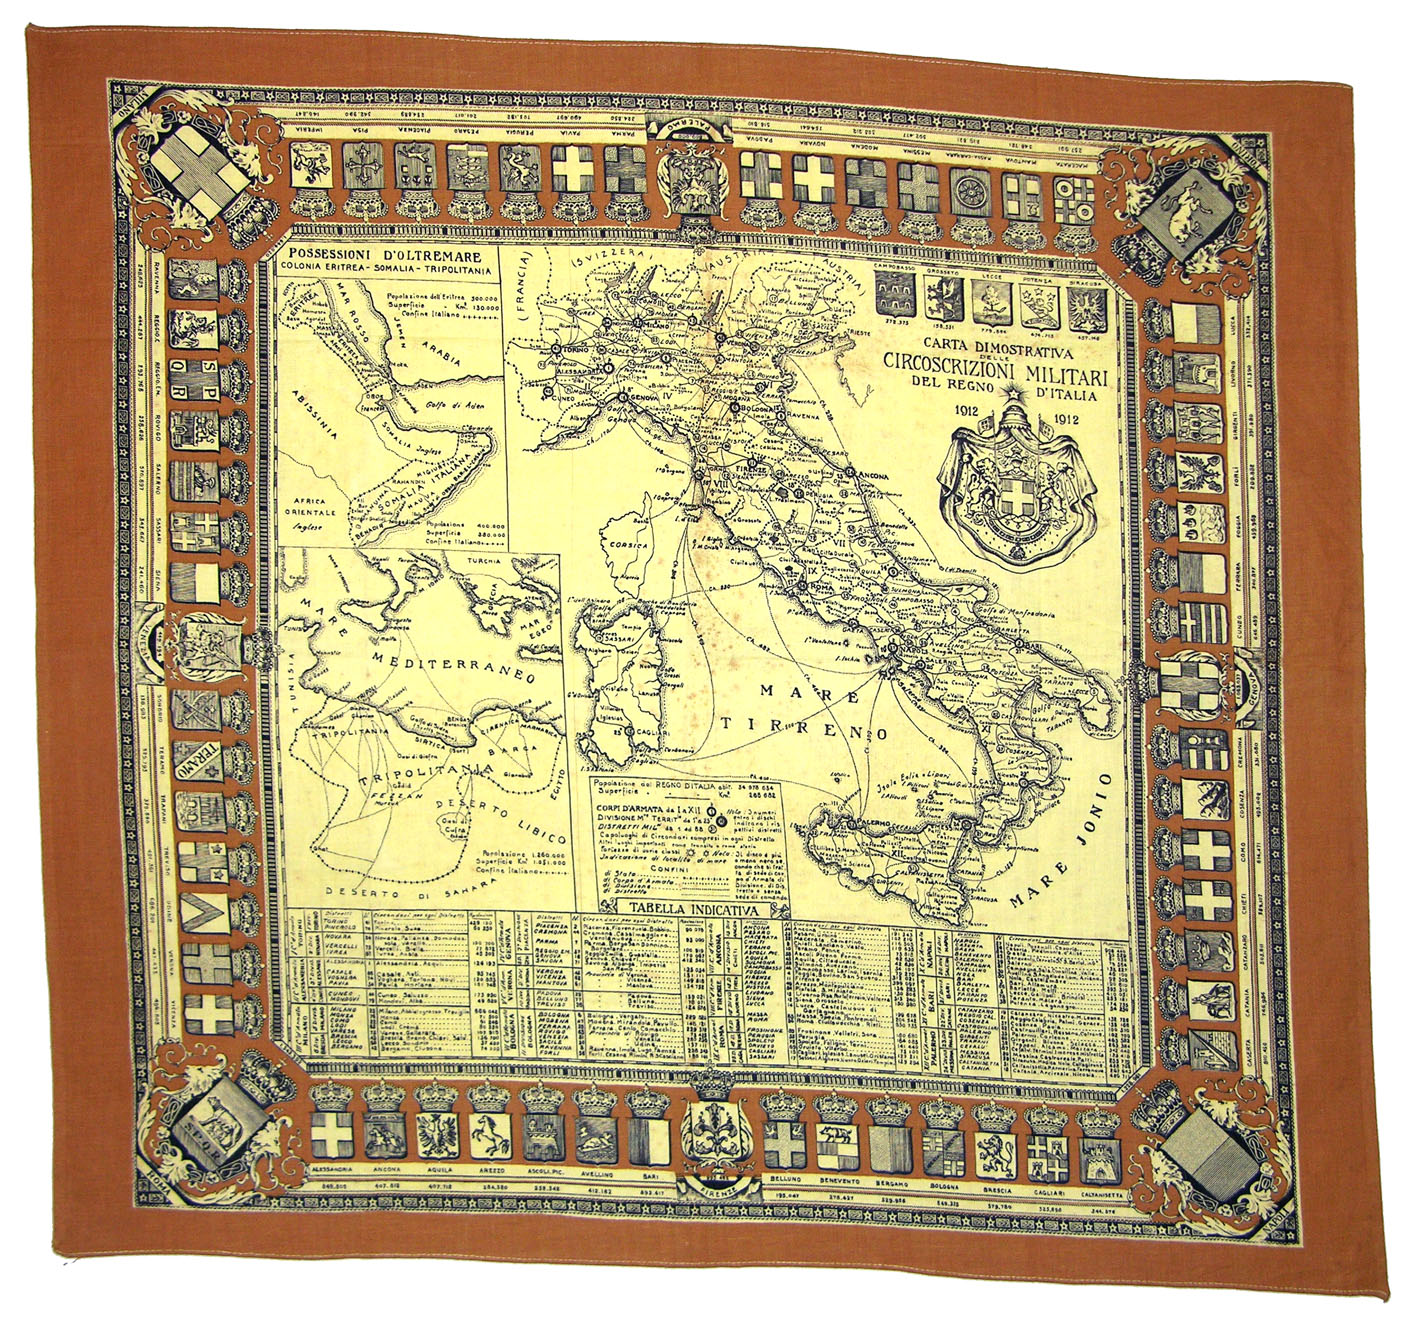
\includegraphics[width=\textwidth]{fazzoletto5_cartaitalia.jpg}
	\caption{Carta d’Italia 1912 Fazzoletto militare italiano n°5 Stamperia E. De Angeli Frua – Milano}
	\label{fig:fazzoletto5_cartaitalia}
\end{figure}

\newpage

\begin{figure}[h]
	\centering
		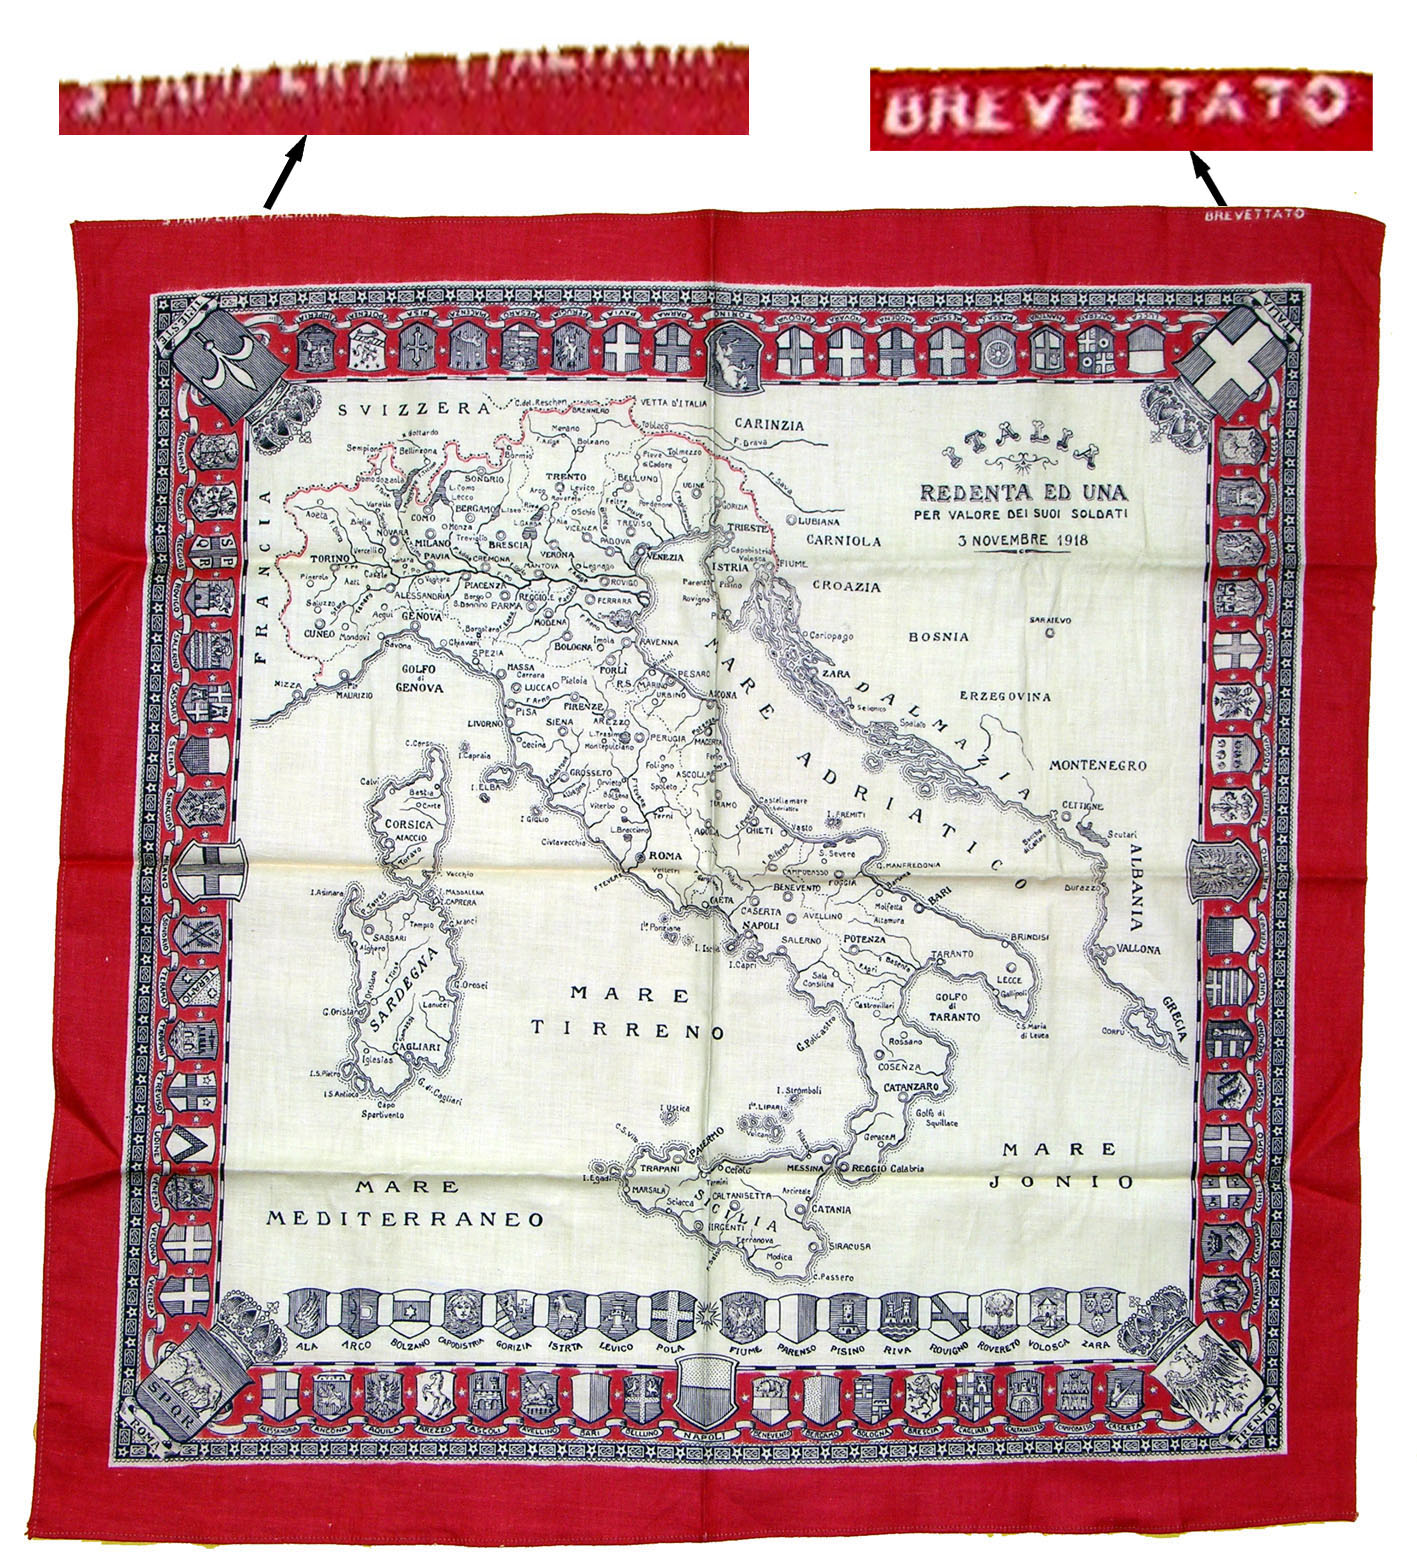
\includegraphics[width=\textwidth]{fazzoletto6_cartaitalia.jpg}
	\caption{Carta d’Italia 1918 Fazzoletto militare italiano n°6 Stamperia E. De Angeli Frua – Milano}
	\label{fig:fazzoletto6_cartaitalia}
\end{figure}

\newpage

\begin{figure}[h]
	\centering
		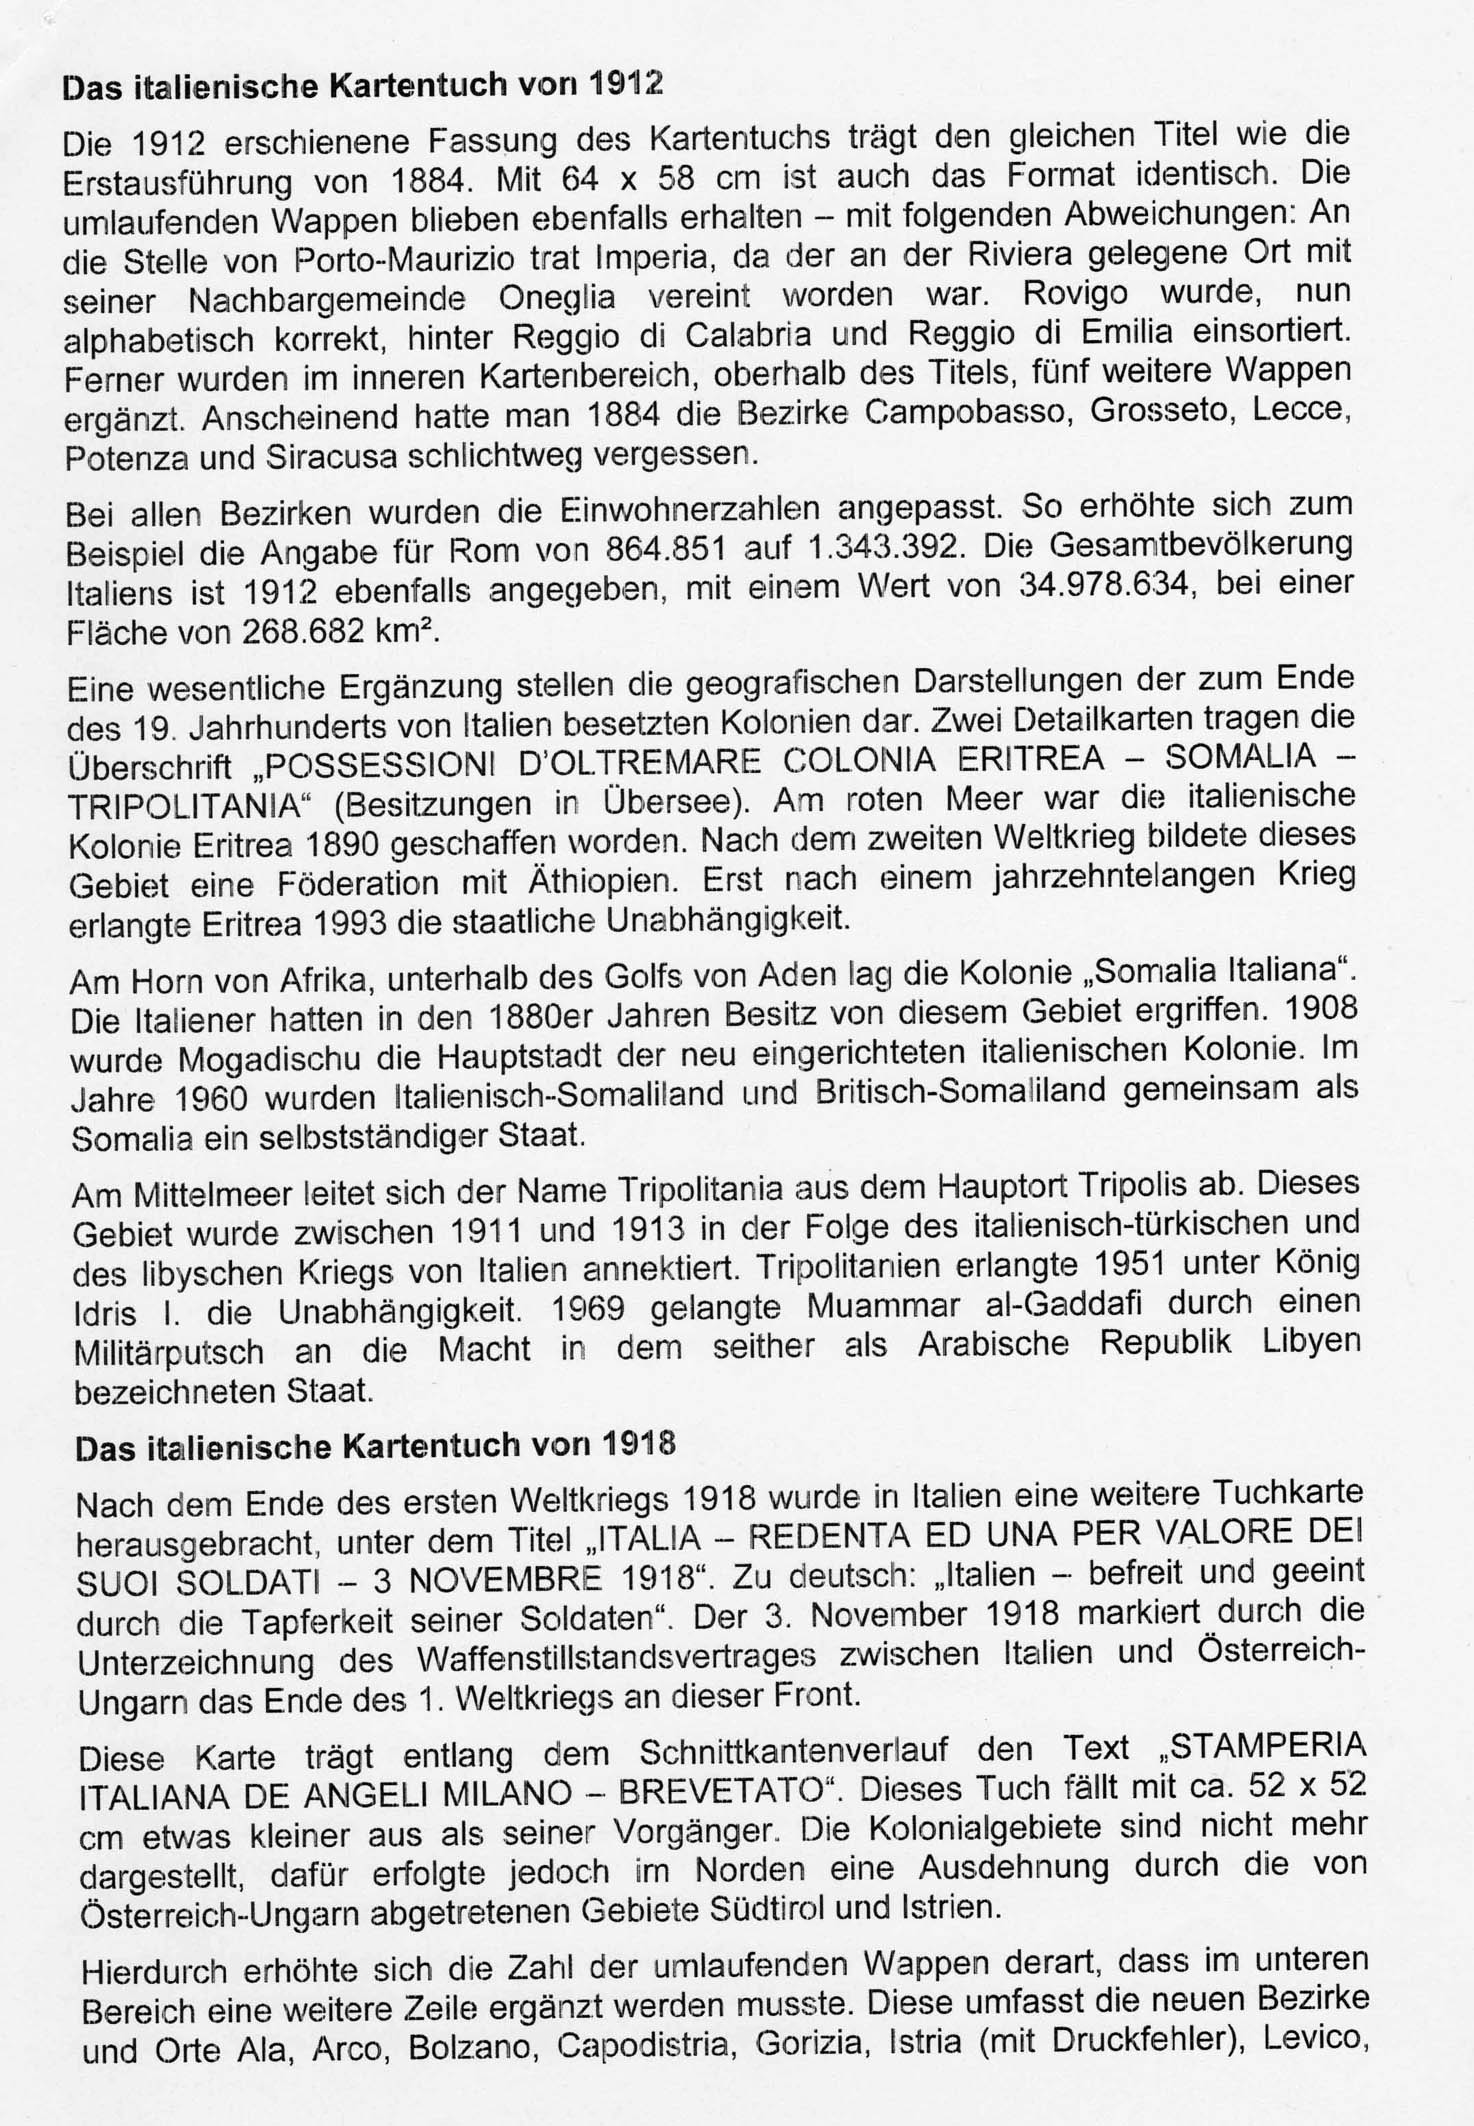
\includegraphics[width=\textwidth]{deangelifrua_7.jpg}
	\caption{}
	\label{fig:deangelifrua_7}
\end{figure}

\newpage

Il fazzoletto italiano con carta geografica del 1912 
(vedi pag. 56)
   
La versione del fazzoletto del 1912 reca lo stesso titolo della prima esecuzione del 1884. Con 64 x 58 cm è anche Io stesso formato. Gli stemmi sono riportati con le seguenti eccezioni: invece di Porto Maurizio c'è Imperia, poiché la città della Riviera era stata riunita con la vicina Oneglia. Rovigo, era ormai in ordine alfabetico correttamente ordinata dietro Reggio Calabria e Reggio Emilia. inoltre, sulle mappe dell'area interna, sopra il titolo, erano aggiunti cinque stemmi. Sembra che nel 1884 i distretti di Campobasso, Grosseto, Lecce, Potenza e Siracusa fossero semplicemente stati dimenticati.
   In tutti i distretti, i dati demografici sono stati rettificati. Per esempio, è aumentata la cifra per Roma da 864 851 a 1.343.392. E' anche riportata la popolazione totale dell'Italia del 1912, con un valore di 34.978.634, con una superficie di 268.682 km2.
   Un complemento essenziale mostra le rappresentazioni geografiche delle colonie italiane della fine del 19 ° Secolo. Due mappe in dettaglio mostrano la scritta “POSSESSIONI D'OLTREMARE COLONIA ERITREA - SOMALIA – TRIPOLITANIA”. Sul Mar Rosso, la colonia italiana d'Eritrea era stata creata nel 1890. 
   Dopo la seconda guerra mondiale questa zona era una federazione con l'Etiopia. Solo dopo un decennio di guerra, l'Eritrea ha ottenuto l'indipendenza nel 1993.
   Nel Corno d'Africa, sotto il Golfo di Aden vi era la colonia della "Somalia Italiana". Gli italiani avevano preso nel 1880 la proprietà di questa zona. Nel 1908 Mogadiscio era diventata la capitale della colonia italiana di nuova costituzione. Nel 1960, la Somalia italiana e la Somalia britannica furono unite come unico stato indipendente con nome Somalia.
   
\newpage

\begin{figure}[h]
	\centering
		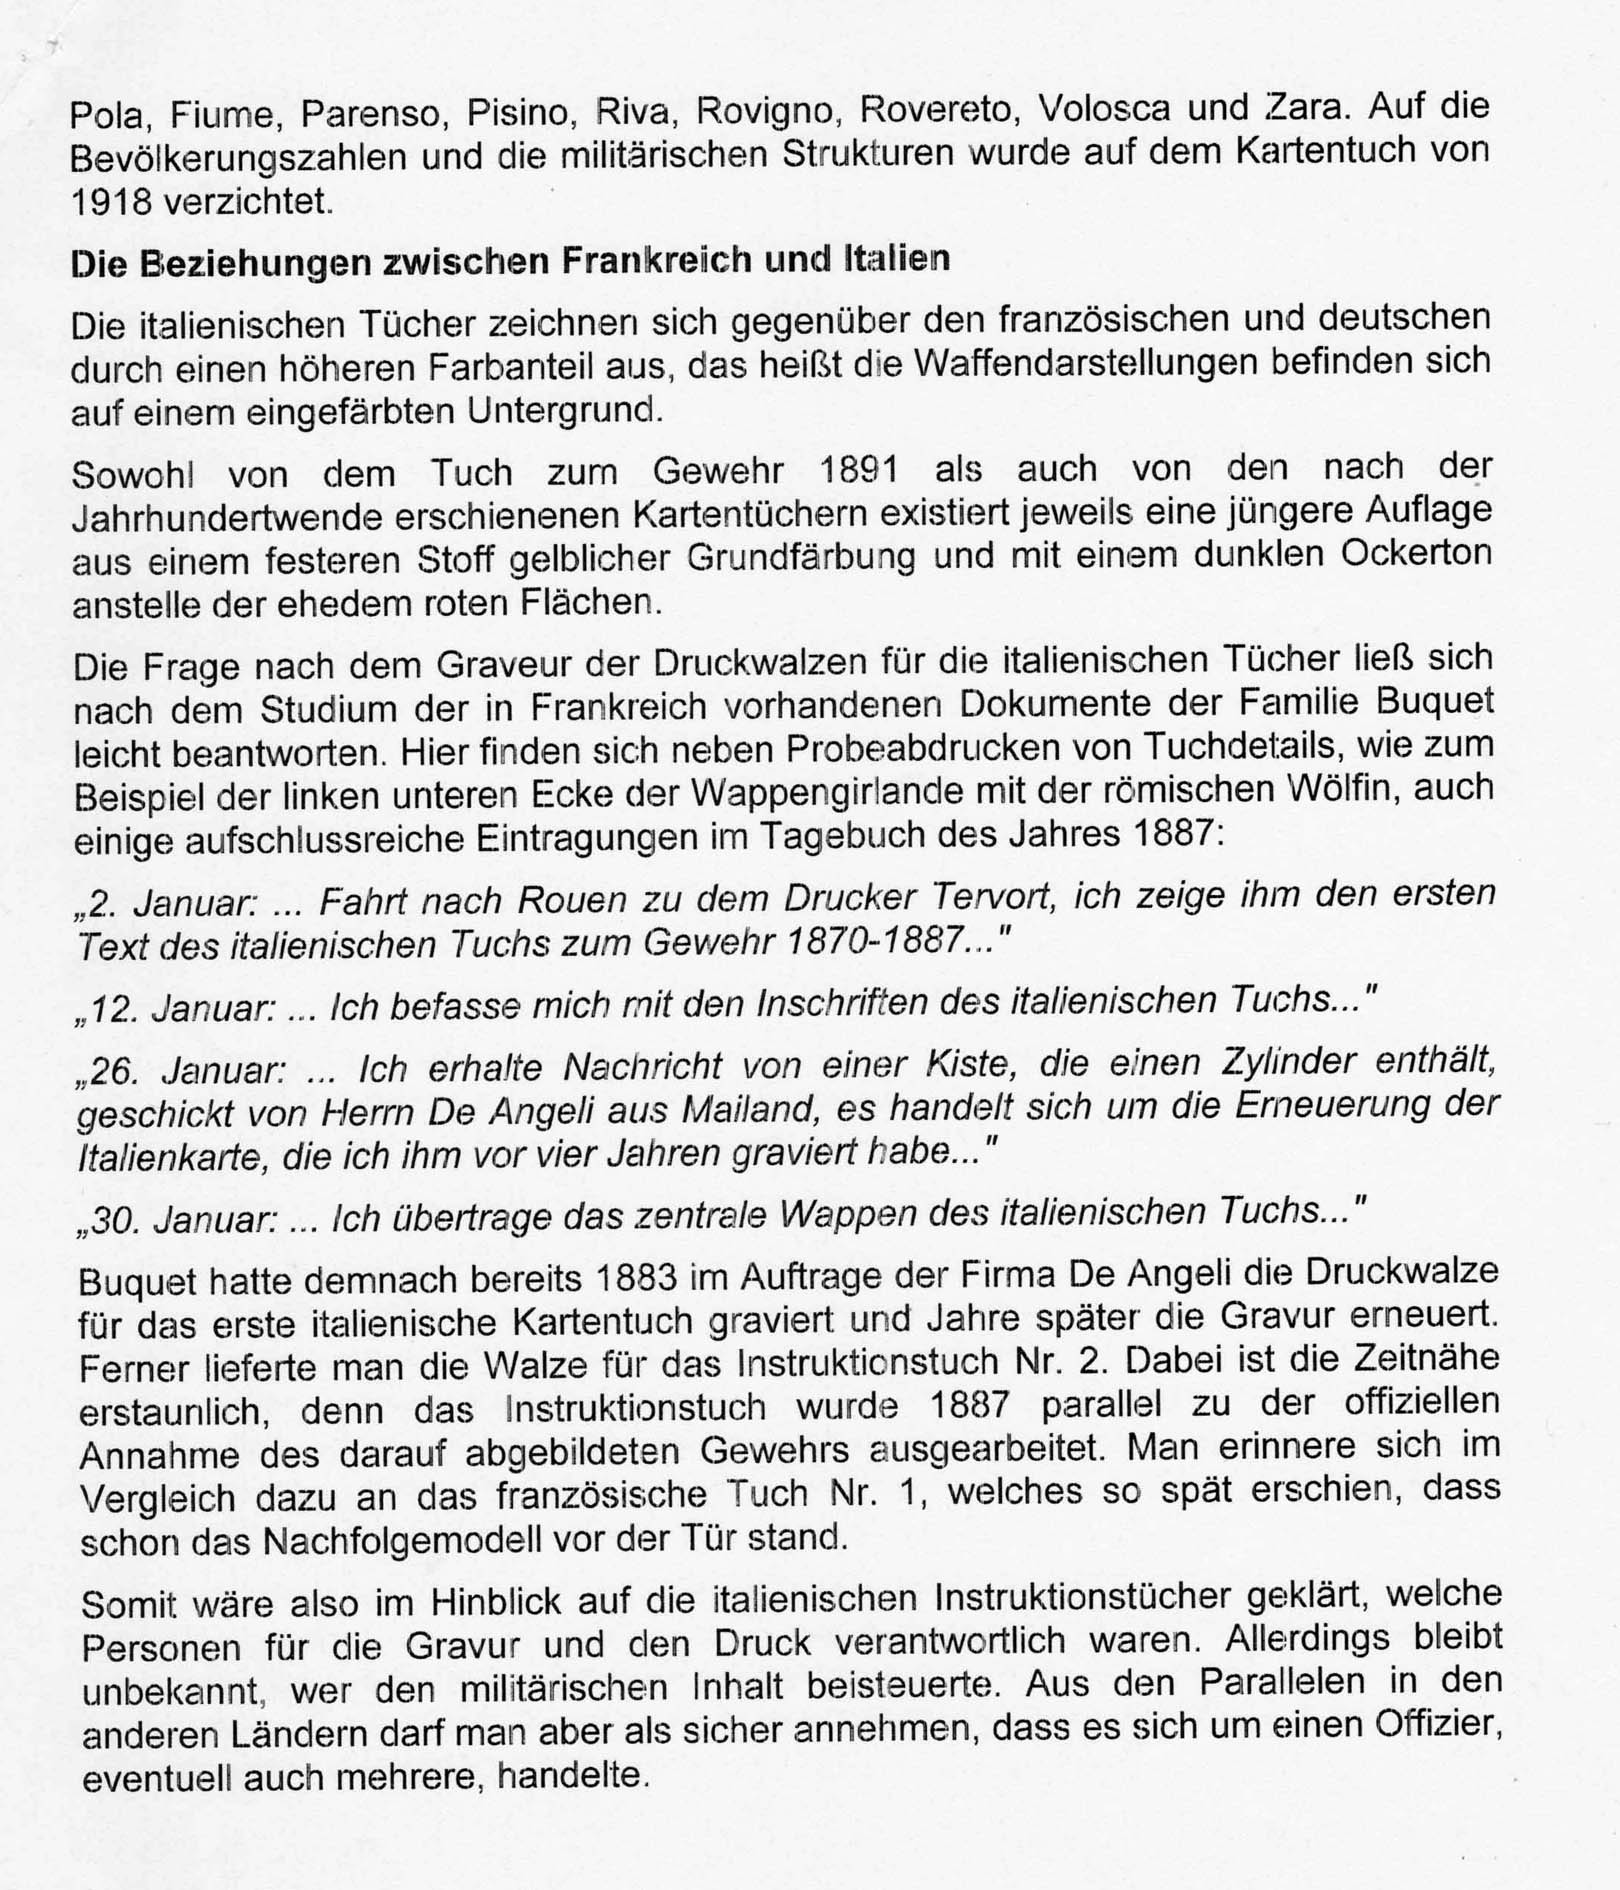
\includegraphics[width=\textwidth]{deangelifrua_8.jpg}
	\caption{}
	\label{fig:deangelifrua_8}
\end{figure}

\newpage

Sul Mediterraneo la Tripolitania deriva dal nome della capitale Tripoli. Questa zona fu annessa nel 1911-1913 sulla scia della guerra italo-turca e della guerra italo-libica. La Tripolitania divenne indipendente col re Idris I nel 1951. Nel 1969 Muammar Gheddafi è arrivato al potere con un colpo di stato militare fondando la Repubblica araba della Libia.

Il fazzoletto italiano con carta geografica del 1918
 (vedi pag.57)

Dopo la fine della prima guerra mondiale in Italia nel 1918, comparve un nuovo fazzoletto, sotto il titolo di "ITALIA - REDENTA ED UNA PER VALORE DEI SUOI SOLDATI - 3 NOVEMBRE 1918". II 3 Novembre 1918 ha segnato con la firma dell'armistizio tra l'Italia e Austria-Ungheria, la fine della prima guerra mondiale su questo fronte.
   Questo fazzoletto porta lungo i bordi il testo "STAMPERIA ITALIANA DE ANGELI MILANO - BREVETTATO".  Questo coincide con un fazzoletto di circa 52 x 52 cm leggermente più piccolo rispetto al suo predecessore. Le colonie non sono più mostrate, ma è stato eseguito un prolungamento a nord con i territori ceduti dall'Austria-Ungheria, l'Alto Adige e l'Istria. Ciò ha aumentato il numero di stemmi in circolo in modo tale che doveva essere aggiunti al fondo di un'altra linea. Ciò comprende i distretti e le nuove città di Ala, Arco, Bolzano, Capodistria, Gorizia, Istria (con errori di stampa), Levico, Pola, Fiume, Parenzo, Pisino, Riva, Rovigno, Rovereto, Volosca e Zara. Sul fazzoletto del 1918 si è rinunciato alla popolazione e alle strutture militari.

I rapporti tra Francia e Italia
  
 I tessuti italiani, in relazione con quelli francesi e tedeschi hanno una maggiore quantità di colore, e ciò significa che gli stemmi sono rappresentazioni su uno sfondo colorato.
   Per il fazzoletto per il fucile nel 1891 così come per quelli pubblicati dopo la fine del secolo, c'è una tiratura più recente di un colore solido di base con un colore giallo ocra scuro al posto dei rosso. La questione dell'incisore dei rulli della stampa per i fazzoletti italiani secondo lo studio dei documenti esistenti fa riferimento alla famiglia francese Buquet. Qui si possono trovare stampe successive di dettagli della stoffa del campione, come ad esempio l'angolo in basso a sinistra dello stemma della lupa romana con la ghirlanda,1 (vedi a pag. 62) e anche alcuni riferimenti nel diario del 1887:  
   “2 Gennaio: ... viaggio a Rouen alla stamperia Tervort, io gli mostro il primo testo del fazzoletto italiano per il fucile 1870-1887... " 
   “12 Gennaio:... Ho a che fare con le iscrizioni del tessuto italiano..”
   “26 Gennaio: ... Ottengo un messaggio di risposta che contiene un cilindro, inviato dal signor De Angeli a Milano, per rinnovare la carta d'Italia, che ho inciso quattro anni fa ...
,, 30 Gennaio:... Trasferisco l'emblema centrale del fazzoletto italiano ...”
   Buquet aveva così inciso nel 1883 per conto di De Angeli, il rullo di pressione per la carta geografica del primo fazzoletto italiano e anni dopo, ha rinnovato l'incisione. Inoltre è stato consegnato il fazzoletto delle istruzioni n ° 2. Qui il poco tempo trascorso è sorprendente, perché nel 1887 è stato preparato il fazzoletto di istruzioni in parallelo con l'adozione formale della carabina raffigurata in esso. Richiama in confronto il fazzoletto francese n ° 1, che sembrava così in ritardo, che c'era già un successore alla porta.
   Così si spiegherebbe in termini di fazzoletti d'istruzione italiani, che le persone che si occupavano di incisione e stampa erano responsabili. Tuttavia, rimane sconosciuto chi abbia contribuito al contenuto militare. Per i paralleli con altri paesi, dobbiamo dare per scontato che si trattasse di un ufficiale, forse anche più d'uno.

\newpage

\begin{figure}[h]
	\centering
		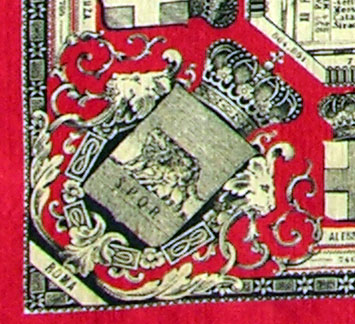
\includegraphics[width=\textwidth]{fazzoletto1_dettaglio.jpg}
	\caption{Dettaglio dell’angolo in basso a sinistra del fazzoletto n°1 (veder pag. 40)}
	\label{fig:fazzoletto1_dettaglio}
\end{figure}

\newpage

\begin{figure}[h]
	\centering
		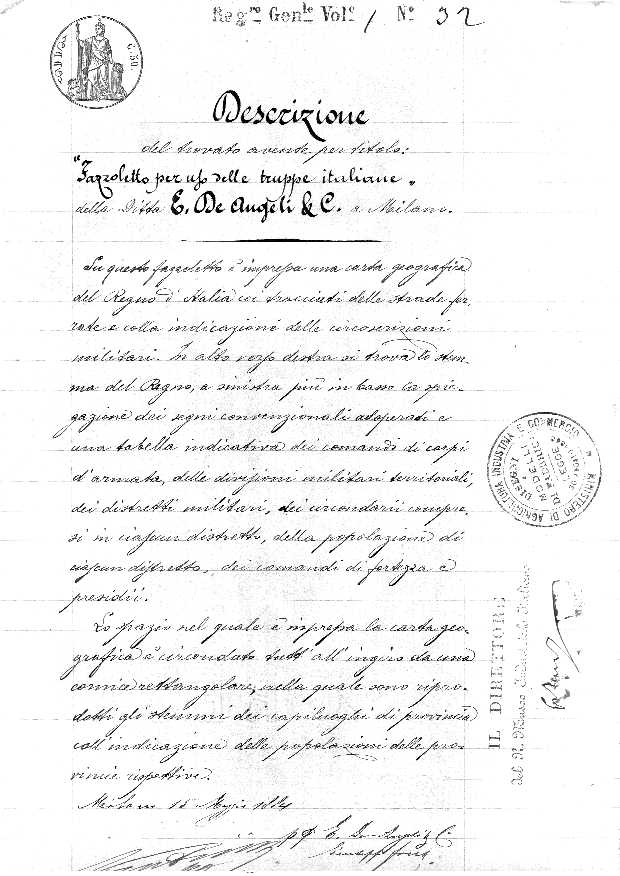
\includegraphics[width=\textwidth]{fazzoletto1_lettera.jpg}
	\caption{15 maggio 1884 Invio al ministero competente della descrizione dettagliata dei contenuti  del fazzoletto n°1}
	\label{fig:fazzoletto1_lettera}
\end{figure}

\newpage

\begin{figure}[h]
	\centering
		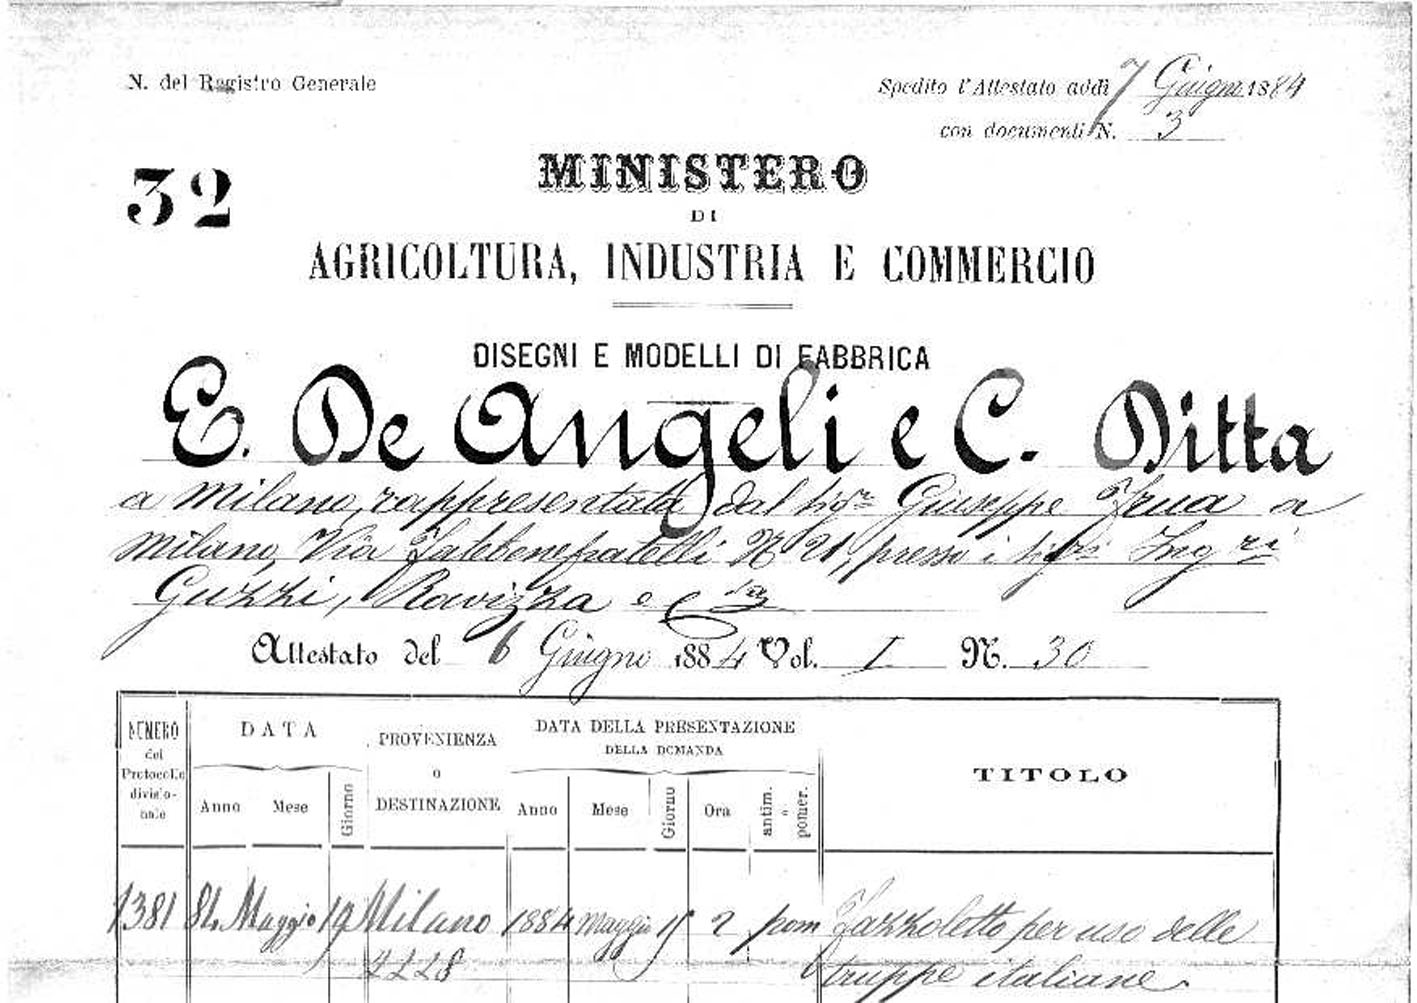
\includegraphics[width=\textwidth]{richiestaautorizzazionestampa.jpg}
	\caption{6 giugno 1884 Richiesta da parte di Giuseppe Frua al ministero competente, per autorizzazione alla stampa dei fazzoletti per istruzione militare italiana}
	\label{fig:richiestaautorizzazionestampa}
\end{figure}

\clearpage







   
   

\clearpage
\chapter[]{I fazzoletti per istruzione militare in Italia}
\graphicspath{ {./images/chapter3/} }

Il testo è stato ricavato dagli articoli di Dirk  Ziesing e da alcune scritte e significativi particolari dei singoli manufatti. 



De Angeli-Frua
   La stamperia italiana per i fazzoletti da istruzione è nata a Saronno, cittadina a nord di Milano,  fondata da Ernesto De Angeli (1849-1907). Egli acquisì la propria formazione professionale grazie al barone Costanzo Cantoni, fondatore dell’industria tessile in Italia. La sua azienda di filatura e tessitura del cotone (cotonificio) nasceva a Castellanza già dal 1845. Nel 1872 venne fondata la “Società Ernesto De Angeli \& C” e nel 1878 denominata “Stamperia milanese per stoffe Cantoni”. De Angeli conquistò una grande reputazione nella sua città natale e nel 1895 venne nominato senatore.
   In questa situazione si deve però citare anche Giuseppe Frua (1855-1937) che, già dall’età di 16 anni, cominciò a conoscere il lavoro della tessitura presso un’azienda tedesca. Al suo rientro in Italia, dapprima trovò un’occupazione nell’azienda tessile Caprotti quindi, nel 1875, entrò a servizio di Eugenio Cantoni, figlio e successore del già nominato Barone. Nel 1879 l’attività Frua venne spostata nella sede di Castellanza. Nel 1883 egli sposò Anna De Angeli e nello stesso tempo divenne procuratore dell’azienda del cognato. Dopodiché, nel 1890 divenne partner della fabbrica tessile dei fratelli Banfi di Legnano (Anonima Frua \& Banfi) e nel 1896 si associano Ernesto De Angeli e Giuseppe Frua concentrando filatura, tessitura e stampa in un’unica azienda, denominata “De Angli-Frua”.
   All’inizio del ventesimo secolo (1900) si sperimentò  anche  la  
produzione  in  proprio  della  seta. A tale scopo    venne acquisto un terreno sul lago di Orta adattando la precedente piantagione di viti e alberi da frutta in gelsi, le cui foglie erano essenziali per l’allevamento dei bruchi. Nello stesso periodo venne inoltre acquistato un sontuoso edificio del 18° secolo sul lago Maggiore, come sede di rappresentanza. Questa villa De Angeli-Frua( a Laveno) – come gran parte degli edifici di origine aziendale a Milano e nei suoi dintorni – esiste ancora oggi.
   In definitiva, nel 1937 figuravano complessivamente cinque fabbriche con 11.000 dipendenti. La fabbrica di Gerenzano, vicino a Milano, divenne oggetto di modello, così come la residenza del direttore e i vicini edifici aziendali, cantine, scuole e un asilo aziendale. A seguito però dei problemi economici dell’industria tessile europea derivante dalla concorrenza asiatica, l’azienda chiuse le porte nel 1970..

Sguardo d’insieme
   La stamperia tessile milanese si dedicò tra l’altro anche ai fazzoletti militari d’istruzione. Per questo, attribuì particolare significato al materiale cartografico, e in seguito venne integrata negli schemi di numerazione italiani. Così nacque nel 1884 il primo fazzoletto con la stampa di una scena militare italiana. Seguirono fazzoletti orientati alla tecniche militari e alla fine vennero nuovamente rappresentati temi geografici.

Fazzoletto italiano n° 1   
La mappa sul fazzoletto in formato 64x58 cm mostra lo stivale italiano, le isole maggiori di Sardegna e Sicilia così come le isole restanti. Oltre alle strade di ordine (classe) 1, 2 e 3 e alle linee ferroviarie, figurano i numeri dei dodici corpi d’armata e le sedi dei comandi e delle fortezze. 
   Il titolo sovrimpresso recita “Carta dimostrativa delle circoscrizioni militari del regno d’Italia 1884”. Tutt’intorno sono rappresentati gli stemmi delle diverse aree d’amministrazione italiane (come dire: le provincie), con i numeri dei rispettivi  abitanti. Negli angoli e al centro  dei lati figurano gli stemmi delle città maggiori: Roma, Firenze, Napoli, Genova, Torino, Palermo, Milano e Venezia. Tra di essi appaiono invece, in ordine alfabetico e in senso orario, tutte le altre città da Alessandria a Vicenza. 


Fazzoletto italiano n° 2

   Il secondo fazzoletto della collezione italiana descrive il fucile della fanteria Modello 1870-87. Esso riporta al centro la scritta “Fucile Modello 1870-87” e sui margini le scritte “Fazzoletto militare N° 2 – (Privativa Industriale)” nonché “Stamperia E. De-Angeli \& C – Milano”. La spiegazione delle due date consiste nel fatto che nel 1887 venne modernizzato il precedente modello del 1870. Un fazzoletto di questa serie solo con il modello originale non venne alla luce,  anche  se  è  certo che esistesse e che venne stampato dalla società Rolffs dedita ai fazzoletti di istruzione austro-ungarici  (vedi fazzoletto 2A di pag.44 ).
   Con il loro aggiornamento, le precedenti armi vennero fornite con il corredo di un caricatore più ampio. Il caricatore con magazzino per quattro cartucce venne sviluppato per il capitano d’artiglieria Giuseppe Vitali. Sullo stesso principio vennero del resto realizzati un anno dopo anche i fucili olandesi Beaumont. Poiché le armi italiane vennero adeguate in grandi quantità,  è molto raro trovare i fucili Vetterli proprio in versione originale. Per la guida del caricatore, la sua carrozzeria riportava un’apertura nella parte inferiore. Per compensare l’indebolimento della struttura, nel legno del fucile venne integrato un piatto metallico. Oltre a ciò si integrò anche una barra per la guida della punta della pallottola, mentre il coperchio di protezione sull’apertura della cassa venne a sua volta rafforzata e compensata con un anello metallico. 
Infine seguirono anche una modifica della leva di sicurezza e l’irrobustimento della baionetta. Il mirino a quadrante già abbozzato da Vecci rappresentò anch’esso una modifica apportata sul Modello 1870 già nel 1881.

Fazzoletto italiano n° 3
  I fucili costruiti nel 1887 vennero modificati già pochi anni dopo attraverso un nuovo fucile a ripetizione. Anche per esso venne creato un nuovo fazzoletto d’istruzione. Esso venne intitolato “Fucile modello 1891”, con riporto sulla fascia    esterna    orizzontale   del   testo   “FAZZOLETTO MILITARE N°3 – (PRIVATIVA INDUSTRIALE), nonché “STAMPERIA E. DE-ANGELI \& C – MILANO”.    Il nuovo fucile italiano venne ufficialmente introdotto in data 29 marzo 1892. Esso è a struttura di caricatore basato sul principio di Mannlicher. Ferdinando von Mannlicher ne ricavò una licenza brevettuale di 300.000 lire. Il sistema di otturazione venne progettato nell’arsenale cittadino dei fucili di Torino sotto la direzione di Salvatore Carcano (1827-1903) e in collaborazione con comandanti e ingegneri militari. In tale circostanza viene talvolta fatto anche il nome di Gustavo Parravicino, Presidente della Commissione per l’approvazione dei nuovi fucili.   Dalla solida costruzione, quest’arma aveva una capacità di magazzino di sei cartucce. Il calibro relativamente piccolo di 6,5x52 mm determinò subito il vantaggio che un singolo soldato poteva portare con sé un consistente quantitativo di munizioni. D’altro lato la sua criticità generalmente riconosciuta consisteva in operazioni di limitata portata balistica. Anche perciò, le cartucce Carcano riportavano il proiettile con la punta arrotondata, ancor oggi usata, e come già da tempo anche altre nazioni avevano fatto con la punta dei loro proiettili.  
   Un ulteriore svantaggio proveniva dalla lunghezza del successivo modello realizzato per la fanteria. Esso riporta un mirino scorrevole con un gittata da 450 a 2000 metri. La misura di 1,60 m dal calcio all’innesto della baionetta derivava dal principio che, negli scontri con la cavalleria, un fante potesse attaccare in modo efficace anche un cavaliere a cavallo. Per la guerra di trincea, che si svilupperà durante la prima guerra mondiale, questa lunghezza sarà invece di forte intralcio. 
  Perciò nella famiglia dei fucili Carcano comparvero delle successive versioni accorciate. Il “Moschetto Cavalleria” venne sviluppato per la Cavalleria nel 1893 e più tardi trasformato anche in fucile da caccia. 
   Tra le altre cose, è interessante la molteplicità delle varianti delle cartucce, sempre stampate sul Fazzoletto Carcano, e riportate nella sua parte bassa.  Accanto alle normali cartucce sottili e pallottole con copertura in nichel (“A pallottola”), c’erano quelle “da esercitazione”, quella “a salve” e le munizioni per tiro a segno. Una particolarità consiste nelle pallottole a sparo singolo e in quelle a mitraglia.
Fazzoletto cartografico italiano del 1912
   L’aspetto del fazzoletto cartografico del 1912 riporta il medesimo titolo della prima stampa del 1884 ed è identico anche il formato di 64x58 cm. La cornice degli stemmi rimane in sostanza la medesima, con le seguenti modifiche: al posto di Porto-Maurizio subentra Imperia, dato che era stata assorbita nella medesima zona rivierasca unitamente alla vicina Oneglia. Rovigo viene collocata dopo Reggio Calabria e Reggio Emilia, adesso in corretto ordine alfabetico. Inoltre, l’area sopra il titolo viene riempita con cinque ulteriori stemmi. A quanto pare infatti erano state semplicemente dimenticate le circoscrizioni di Campobasso, Grosseto, Lecce, Potenza e Siracusa.
   A ciascuna circoscrizione viene inoltre associato il numero dei residenti. Così, per esempio per Roma, figura l’indicazione di 864.851 abitanti.  Viene  inoltre  riportato  il numero complessivo degli italiani nel 1912, per un valore di 34.978.634 unità con una densità di 268.682 persone a kmq.
   È anche presente un essenziale completamento alla carta geografica con il riporto delle colonie possedute dall’Italia alla fine del 19° secolo. Due dettagliate carte geografiche riportano il sovra titolo “POSSESSIONI D’OLTRE MARE COLONIA ERITREA – SOMALIA - TRIPOLITANIA” (possedimenti d’oltre mare). Sul Mar Rosso era stata acquisita la colonia italiana d’Eritrea nel 1890. Dopo la seconda guerra mondiale questo territorio costituì una federazione con gli Etiopi. Solo dopo una guerra di una decina d’anni l’Eritrea divenne uno stato indipendente.   Sul Corno d’Africa, al di sotto del Golfo di Aden, si trovava la colonia “Somalia Italiana”.  
Fazzoletto cartografico italiano del 1918
   Alla fine della prima guerra mondiale venne prodotto un altro fazzoletto cartografico italiano, con titolo “ITALIA – REDENTA E UNA PER VALORE DEI SUOI SOLDATI – 3 NOVEMBRE 1918”. Il 3 novembre 1918 segnò attraverso la firma dell’armistizio tra l’Italia e l’Austria-Ungheria la fine della prima guerra mondiale su questo fronte.
   Questa Carta riporta lungo la cornice la scritta “STAMPERIA ITALIANA DE ANGELI MILANO – BREVETTATO”. Questo fazzoletto con lati di circa 52x52 cm è leggermente più piccolo del suo predecessore. Le aree coloniali  non  sono  più  rappresentate, ma in cambio seguì un allargamento nel NORD attraverso i territori de Sud Tirolo e del’Istria sottratti all’Austria-Ungheria.  
   Parimenti aumentò il numero degli stendardi di cornice, che venne organizzato in una nuova fila disposta nell’area inferiore del fazzoletto. Essa comprende le nuove circoscrizioni e sedi di Ala, Arco, Bolzano, Capodistria, Gorizia, Istria (con un errore di stampa), Levico, Pola, Fiume, Parenzo, Pisino, Riva, Rovigo, Rovereto, Volosca e Zara. Nel fazzoletto del 1918 si soprassedette al riporto del numero degli abitanti e delle strutture militari. 

\newpage

Nota esplicativa  
   Del fazzoletto sulla cavalleria (vedi pag. 52) l’unica cosa certa è che il prodotto è della stamperia E. De Angeli. Attualmente non siamo in grado di riportare altre documentazioni e/o spiegazioni. La stessa cosa vale per il manufatto sulle armi pesanti che viene effigiato a pagina 53. Questi due fazzoletti però documentano che oltre ai fazzoletti cartografici venivano stampati anche quelli dedicati a reparti militari specifici.
   
\begin{figure}[h]
	\centering
		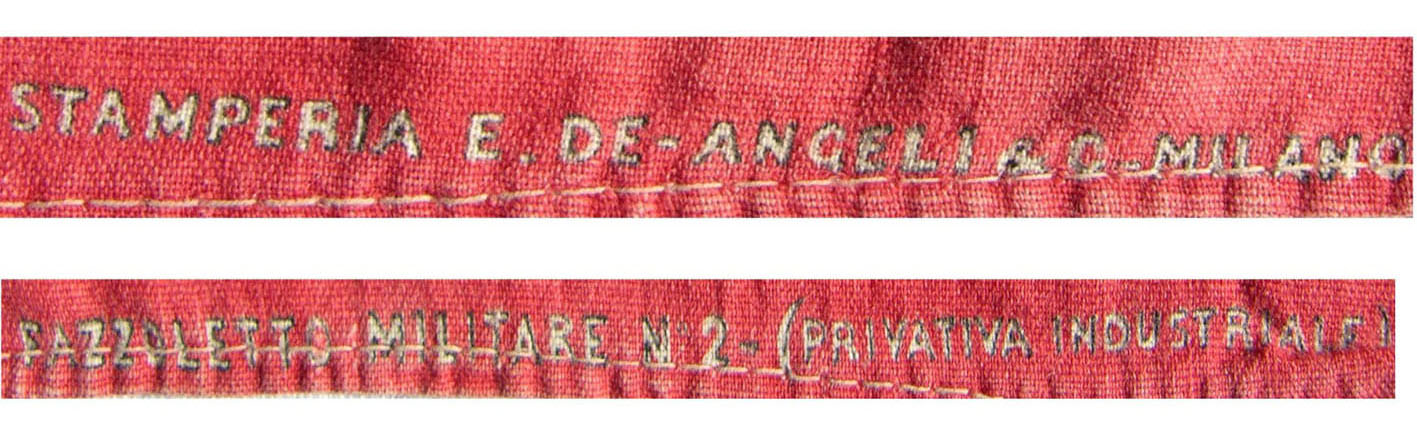
\includegraphics[width=\textwidth]{fazzoletto2_particolare.jpg}
	\caption{Particolare fazzoletto militare italiano n° 2. Certificazione della produzione stampata sul bordo inferiore.}
	\label{fig:fazzoletto2_particolare}
\end{figure}

\newpage

\begin{figure}[h]
	\centering
		
\includegraphics[width=\textwidth]{fazzoletto1_particolare.jpg}
	\caption{Particolare del fazzoletto militare n° 1}
	\label{fig:fazzoletto1_particolare}
\end{figure}

\newpage

\begin{figure}[h]
	\centering
		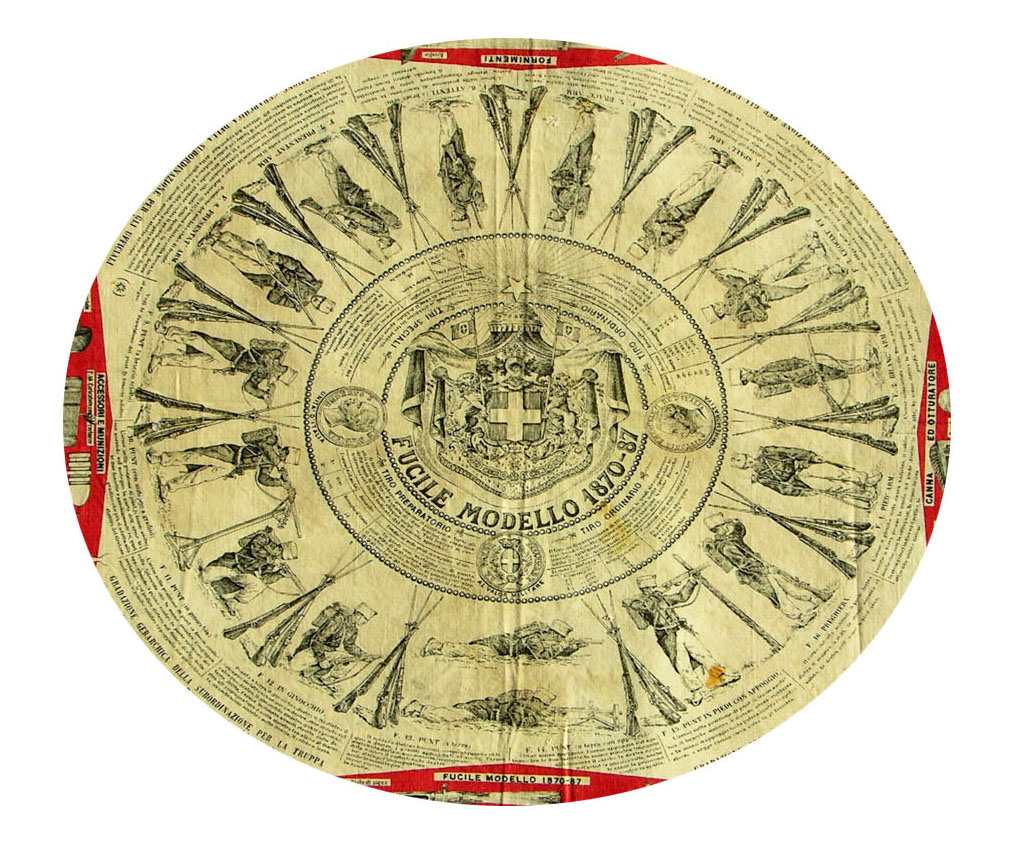
\includegraphics[width=\textwidth]{fazzoletto2_particolare_2.jpg}
	\caption{Particolare del fazzoletto  militare n° 2}
	\label{fig:fazzoletto2_particolare_2}
\end{figure}

\newpage

\begin{figure}[h]
	\centering
		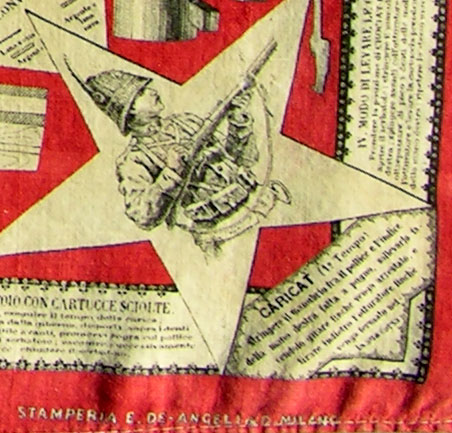
\includegraphics[width=\textwidth]{fazzoletto2_particolare_3.jpg}
	\centering
		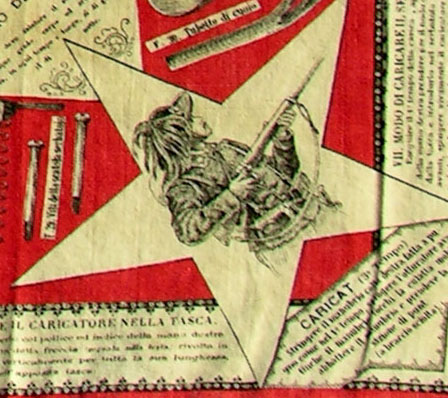
\includegraphics[width=\textwidth]{fazzoletto2_particolare_4.jpg}
	\caption{Particolari del fazzoletto militare n° 2. È evidente il nome del produttore nel bordo inferiore del modello in alto}
	\label{fig:fazzoletto2_particolare_3_4}
\end{figure}

\newpage

\begin{figure}[h]
	\centering
		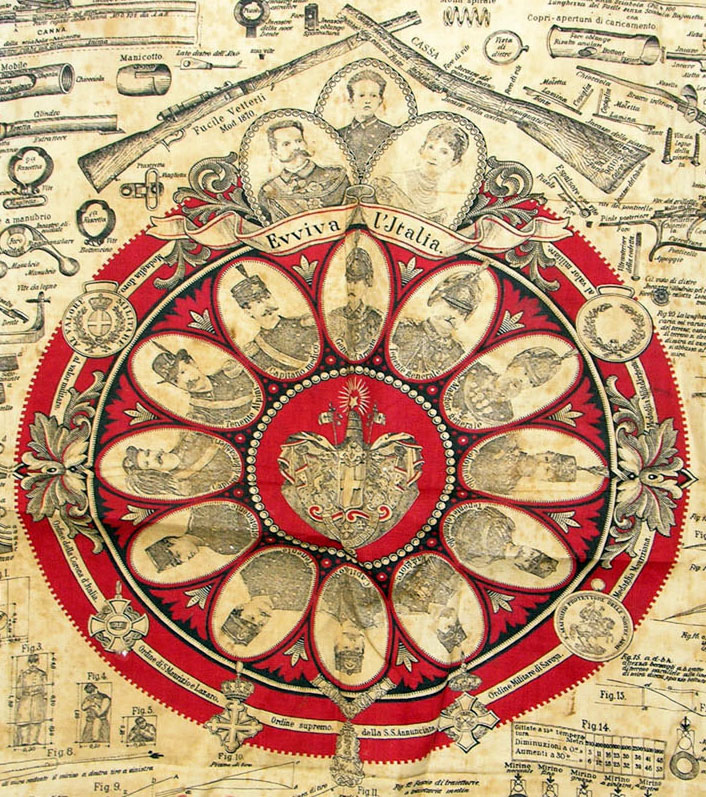
\includegraphics[width=\textwidth]{fazzoletto2A_particolare.jpg}
	\caption{Particolare del fazzoletto militare n°2°A.}
	\label{fig:fazzoletto2A_particolare}
\end{figure}

\newpage

\begin{figure}[h]
	\centering
		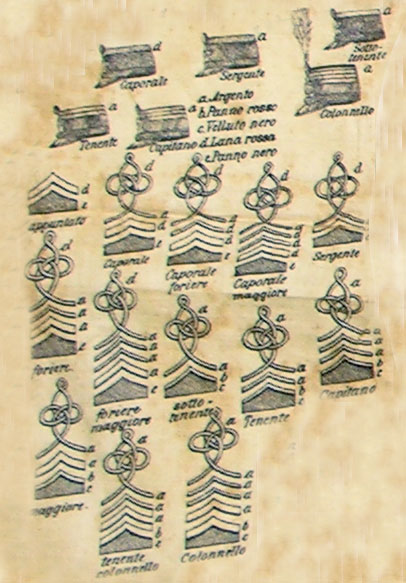
\includegraphics[width=\textwidth]{fazzoletto2A_particolare_2.jpg}
	\caption{}
	\label{fig:fazzoletto2A_particolare_2}
\end{figure}

\newpage

Altri particolari del fazzoletto militare  n° 2A

\begin{figure}[h]
	\centering
		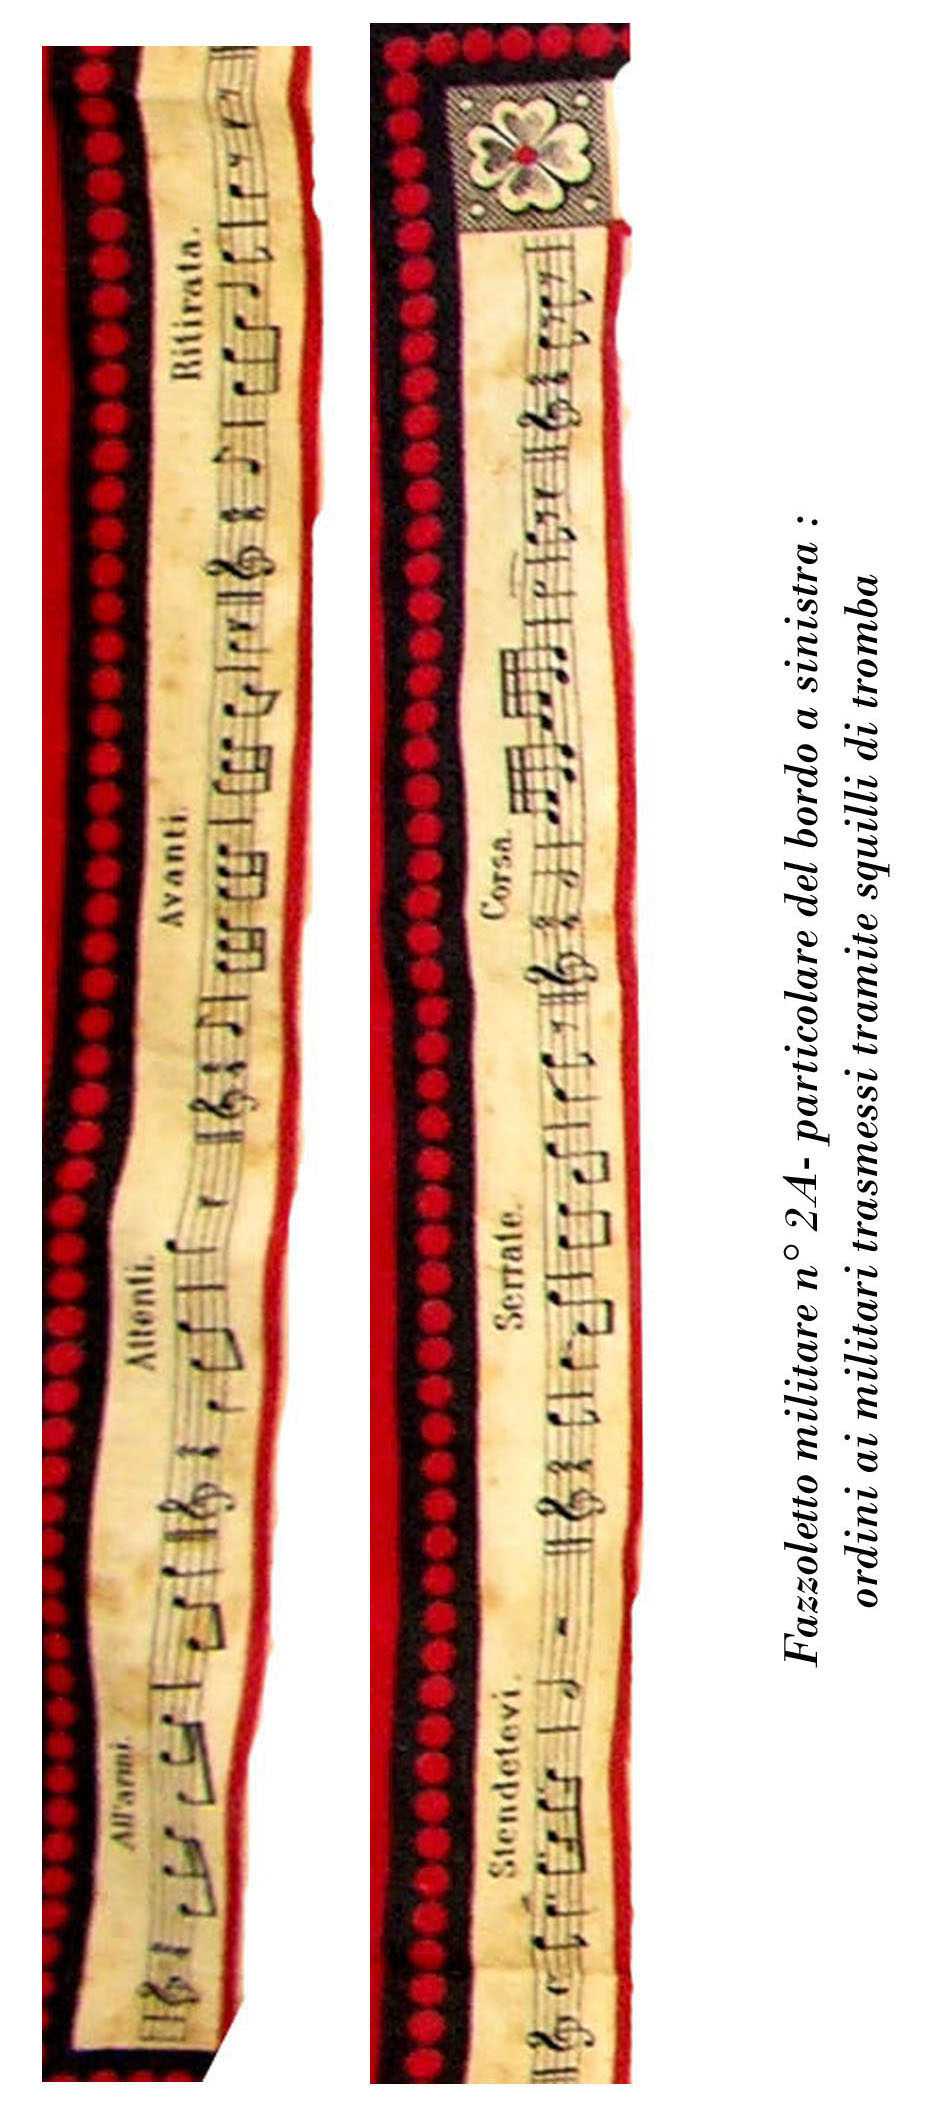
\includegraphics[width=\textwidth]{fazzoletto2A_particolare_3.jpg}
	\caption{}
	\label{fig:fazzoletto2A_particolare_3}
\end{figure}

\newpage

\begin{figure}[h]
	\centering
		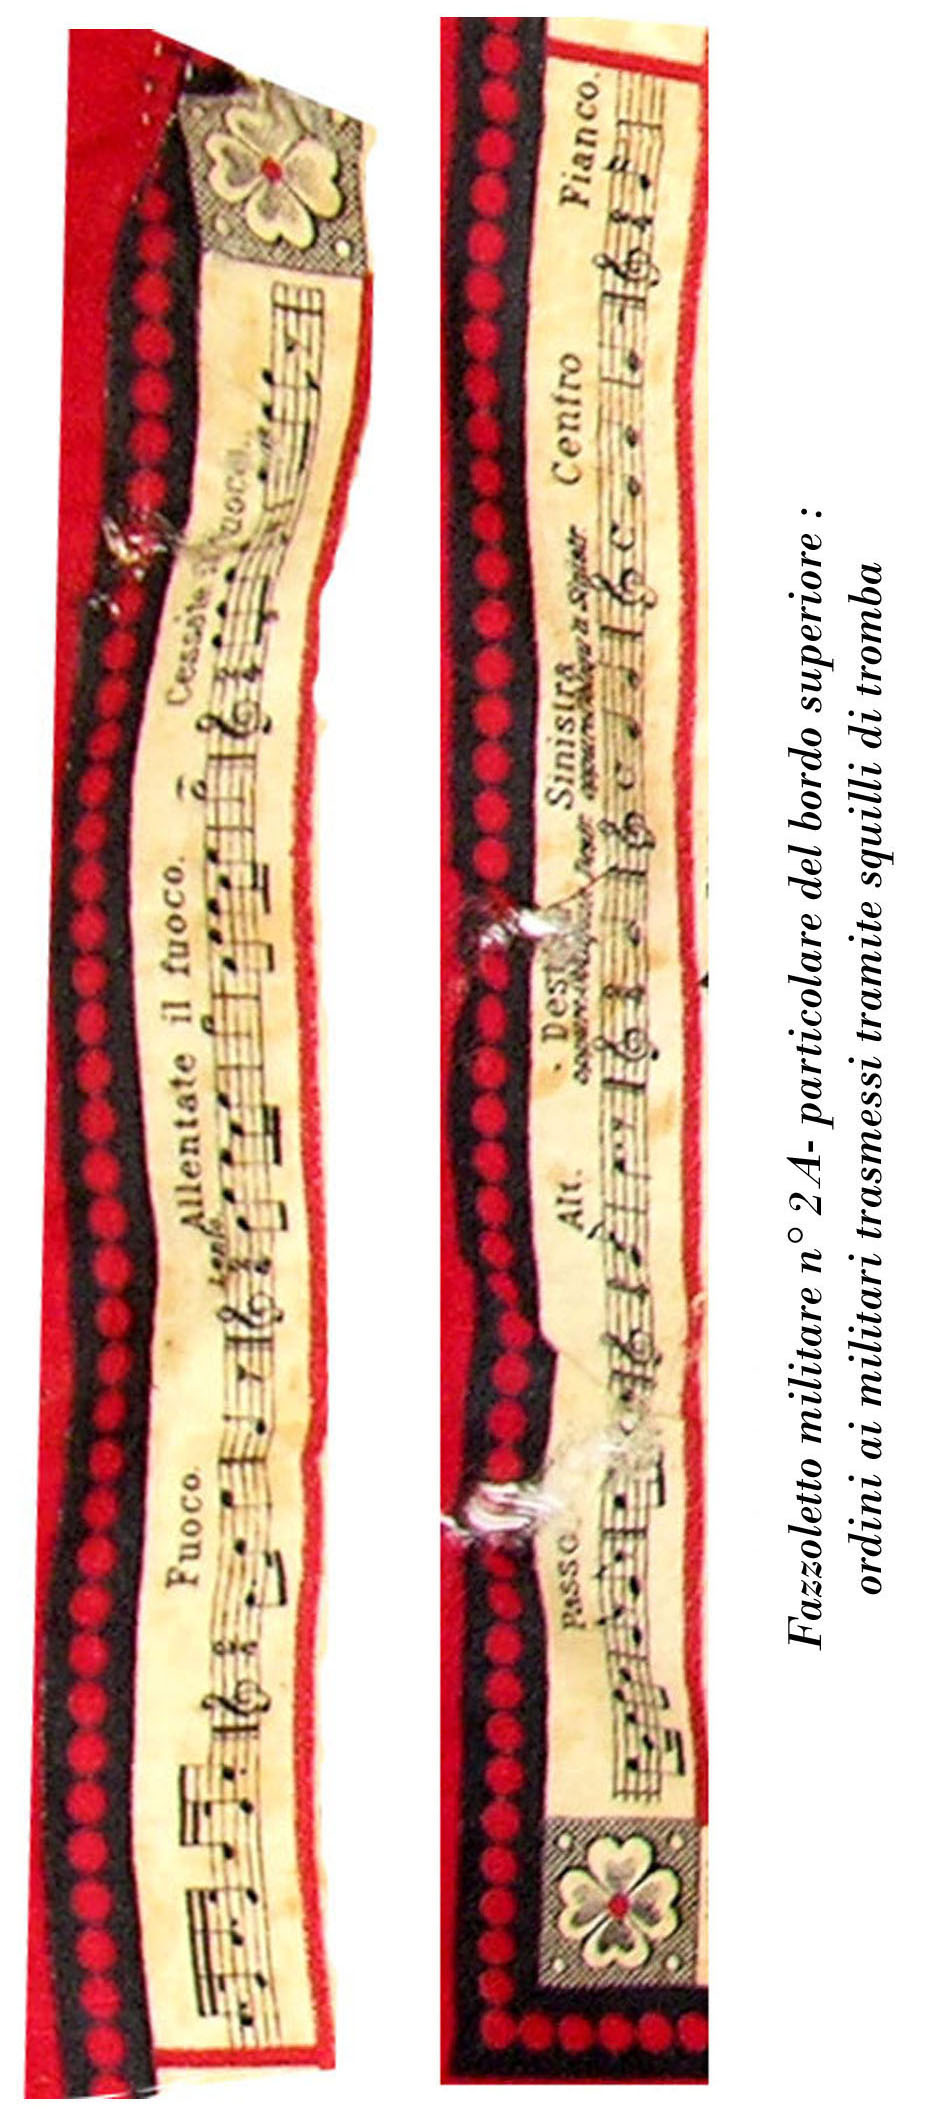
\includegraphics[width=\textwidth]{fazzoletto2A_particolare_4.jpg}
	\caption{}
	\label{fig:fazzoletto2A_particolare_4}
\end{figure}

\newpage

\begin{figure}[h]
	\centering
		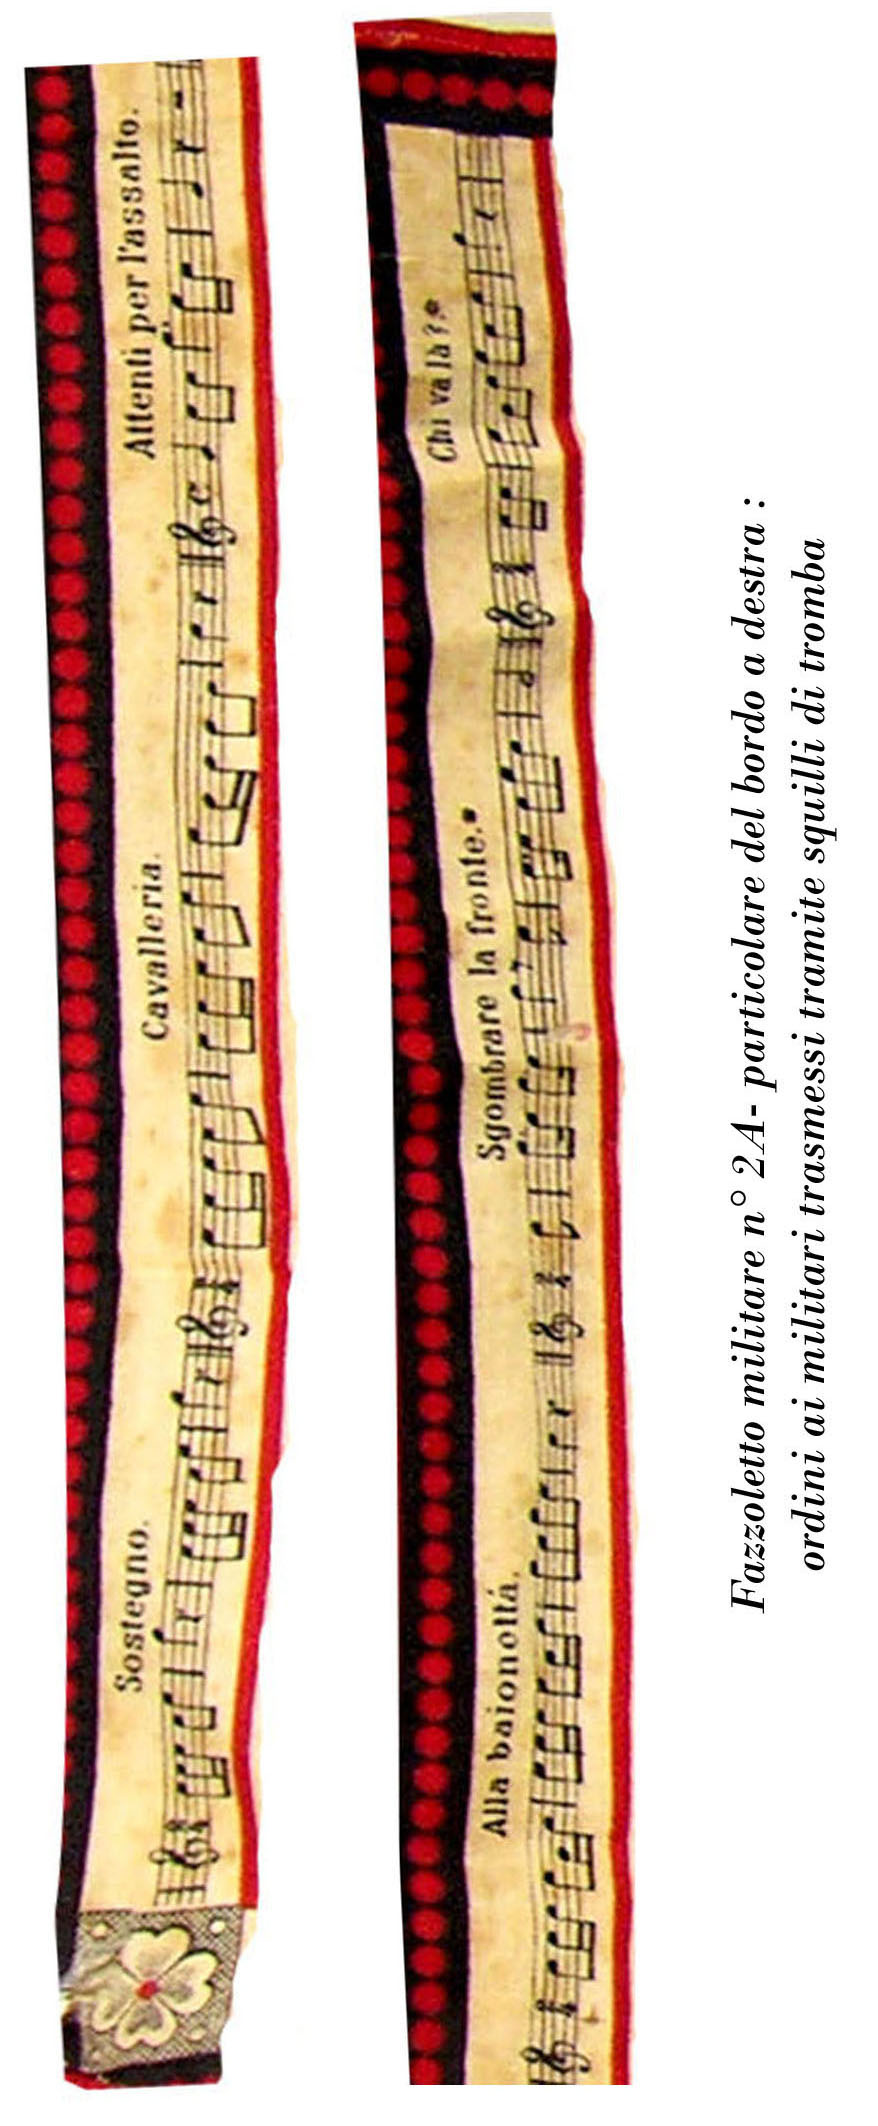
\includegraphics[width=\textwidth]{fazzoletto2A_particolare_5.jpg}
	\caption{}
	\label{fig:fazzoletto2A_particolare_5}
\end{figure}

\newpage

\begin{figure}[h]
	\centering
		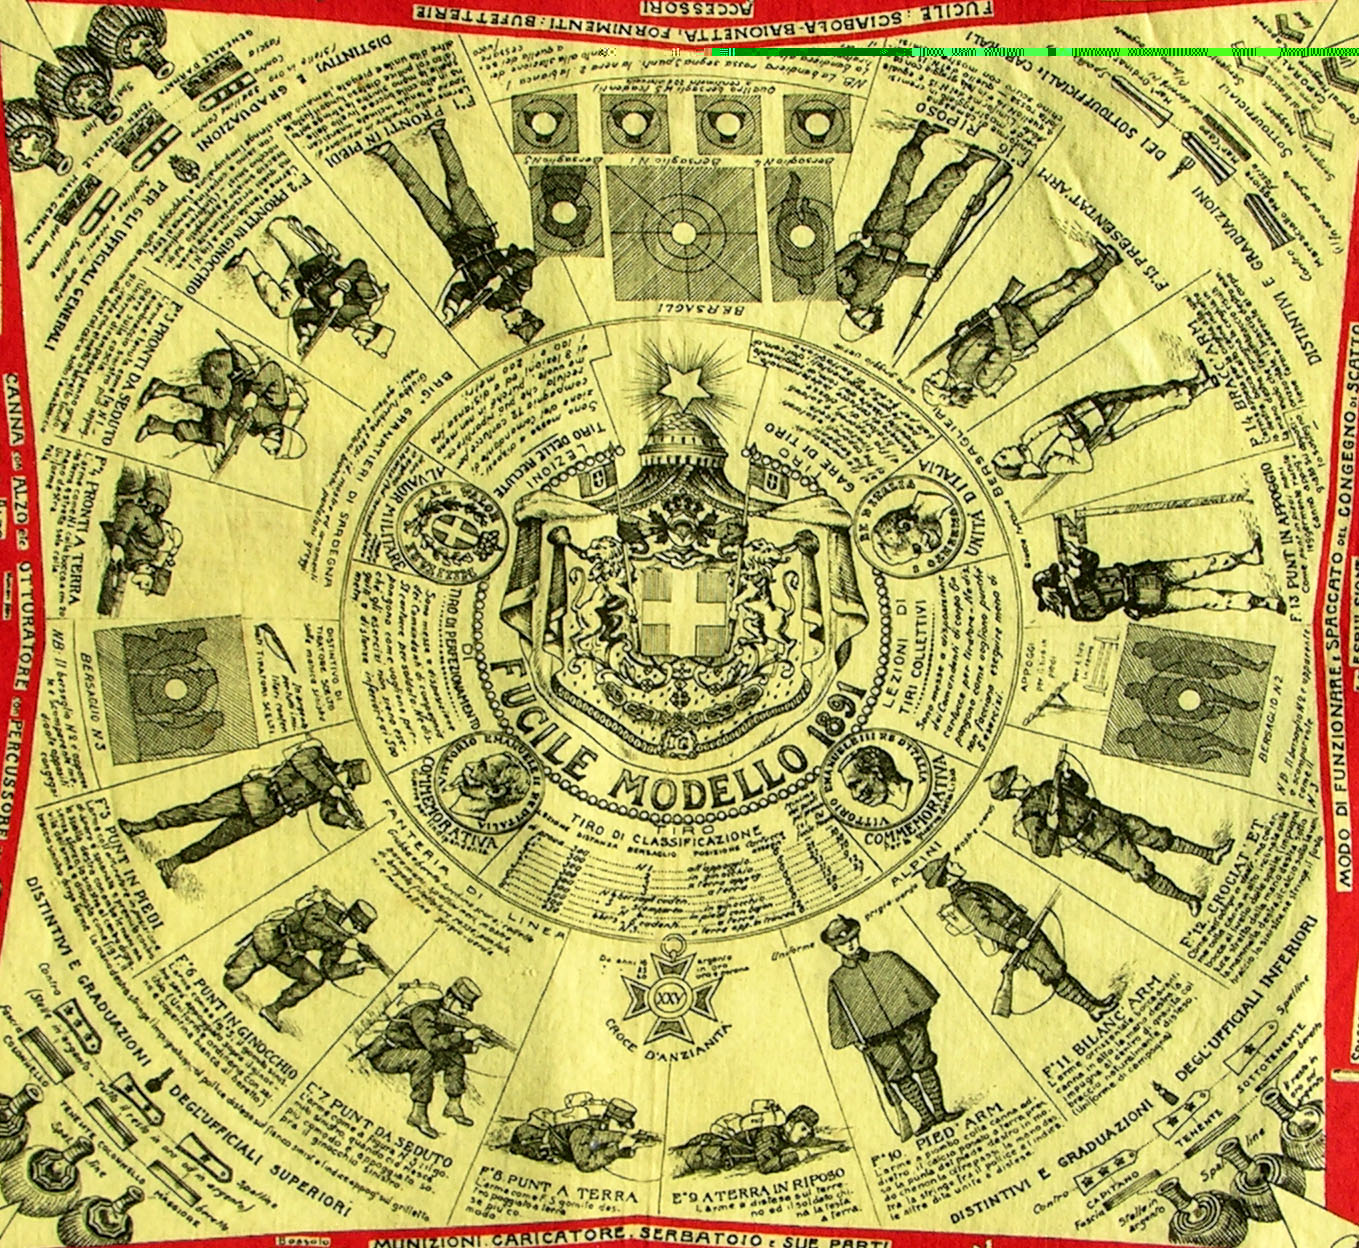
\includegraphics[width=\textwidth]{fazzoletto3_particolare.jpg}
	\caption{Particolare del fazzoletto militare n°3}
	\label{fig:fazzoletto3_particolare}
\end{figure}

\newpage

\begin{figure}[h]
	\centering
		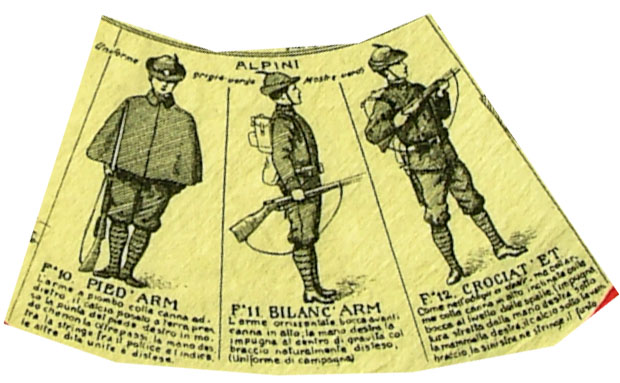
\includegraphics[width=\textwidth]{fazzoletto3_particolare_2.jpg}
	\centering
		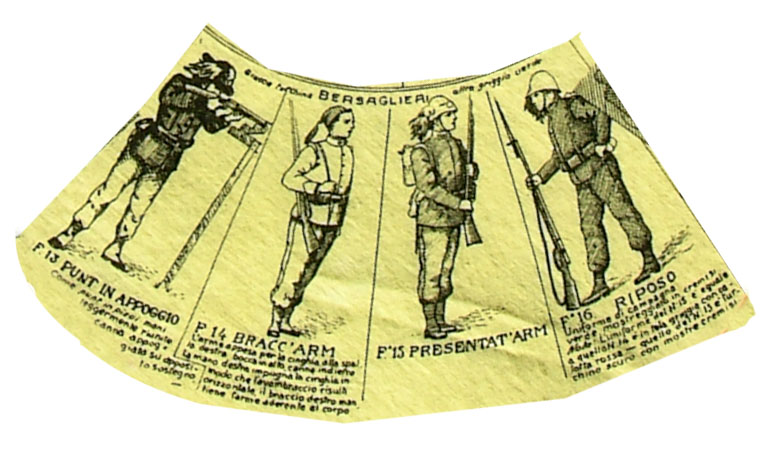
\includegraphics[width=\textwidth]{fazzoletto3_particolare_3.jpg}
	\caption{Altri particolari del fazzoletto militare n° 3}
	\label{fig:fazzoletto3_particolare_2_3}
\end{figure}

\newpage

\begin{figure}[h]
	\centering
		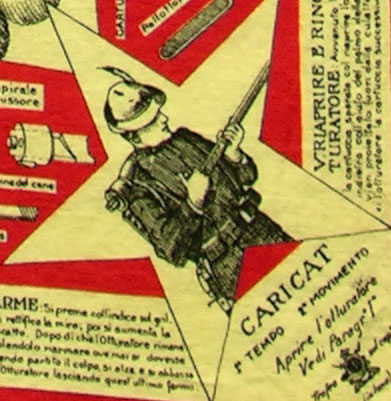
\includegraphics[width=\textwidth]{fazzoletto3_particolare_4.jpg}
	\centering
		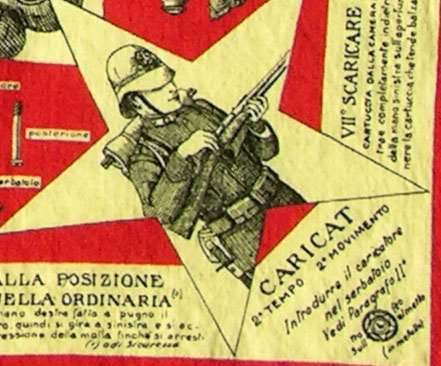
\includegraphics[width=\textwidth]{fazzoletto3_particolare_5.jpg}
	\caption{Altri particolari del fazzoletto militare n° 3}
	\label{fig:fazzoletto3_particolare_4_5}
\end{figure}

\newpage

\begin{figure}[h]
	\centering
		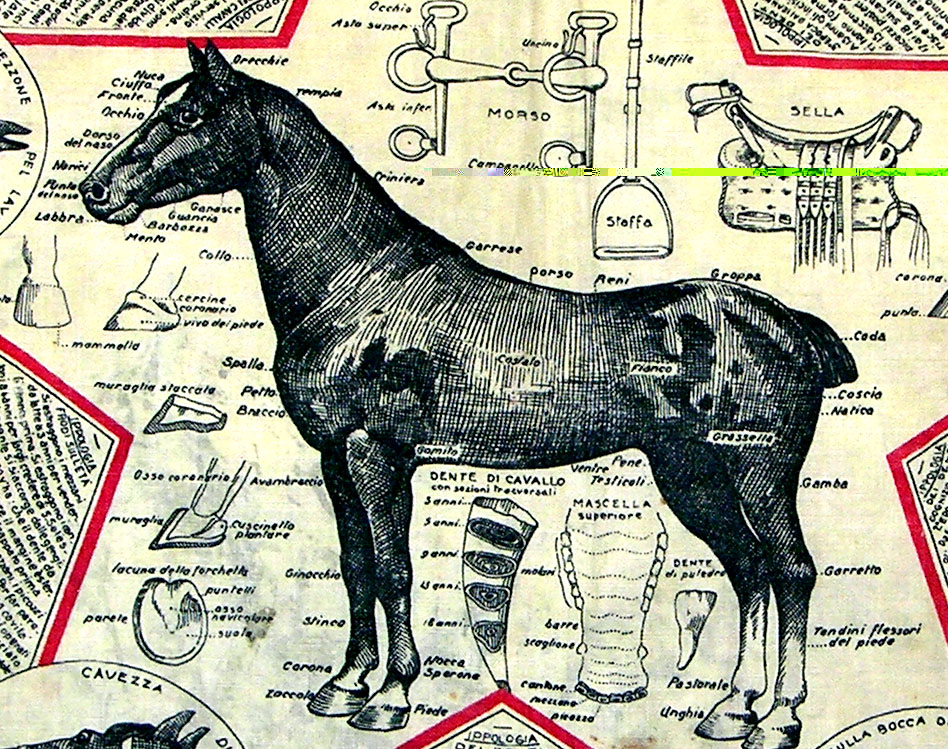
\includegraphics[width=\textwidth]{fazzoletto4_particolare.jpg}
	\caption{Particolare del fazzoletto militare n°4}
	\label{fig:fazzoletto4_particolare}
\end{figure}

\newpage

\begin{figure}[h]
	\centering
		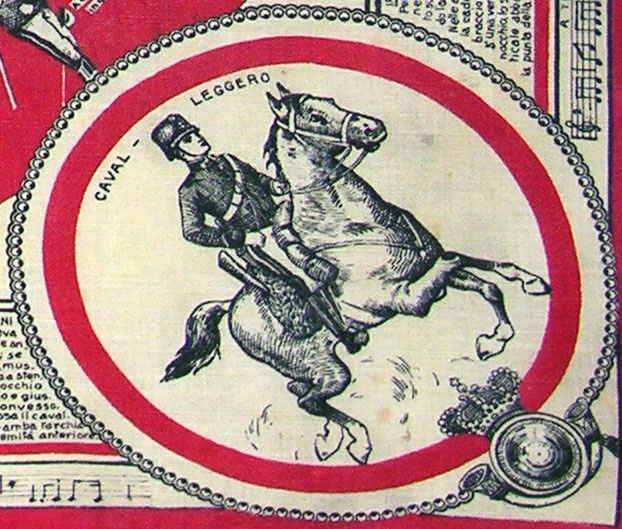
\includegraphics[width=\textwidth]{fazzoletto4_particolare_2.jpg}
	\centering
		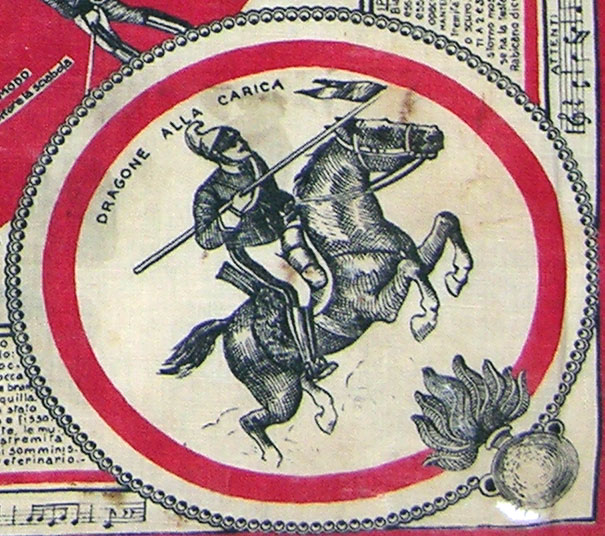
\includegraphics[width=\textwidth]{fazzoletto4_particolare_3.jpg}
	\caption{Particolari del fazzoletto militare n° 4}
	\label{fig:fazzoletto4_particolare_2_3}
\end{figure}

\newpage

\begin{figure}[h]
	\centering
		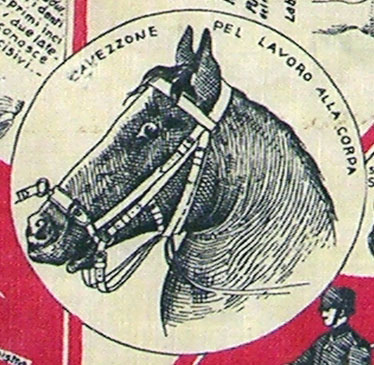
\includegraphics[width=\textwidth]{fazzoletto4_particolare_4.jpg}
	\centering
		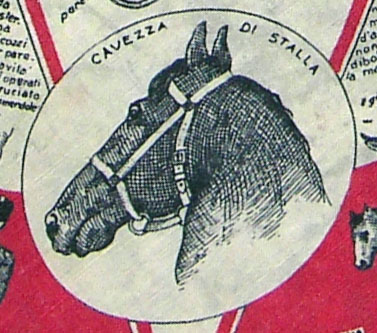
\includegraphics[width=\textwidth]{fazzoletto4_particolare_5.jpg}
	\caption{Dettagli d’immagini del fazzoletto militare n° 4}
	\label{fig:fazzoletto4_particolare_4_5}
\end{figure}

\newpage

\begin{figure}[h]
	\centering
		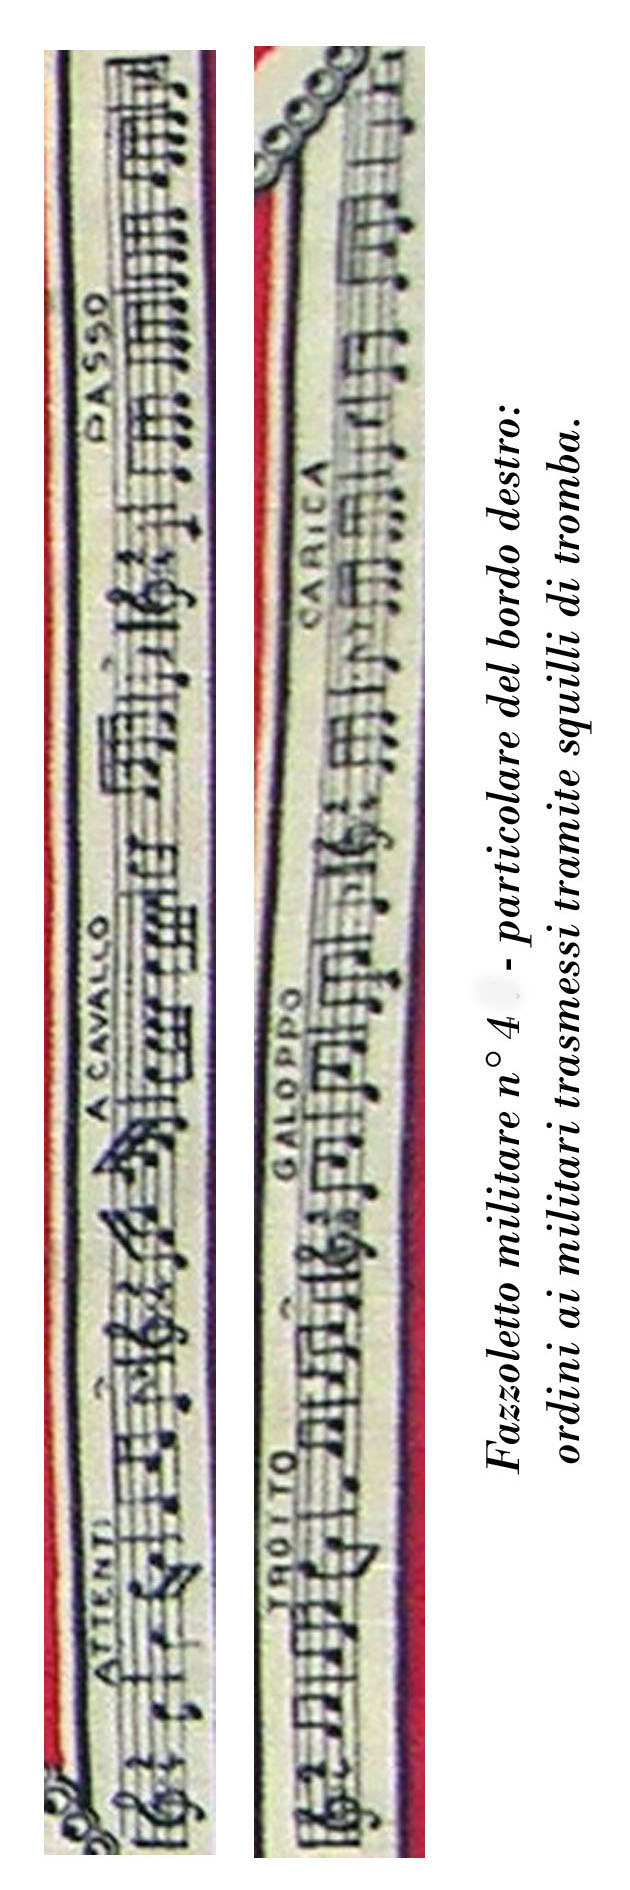
\includegraphics[width=\textwidth]{fazzoletto4_particolare_6.jpg}
	\caption{}
	\label{fig:fazzoletto4_particolare_6}
\end{figure}

\newpage

\begin{figure}[h]
	\centering
		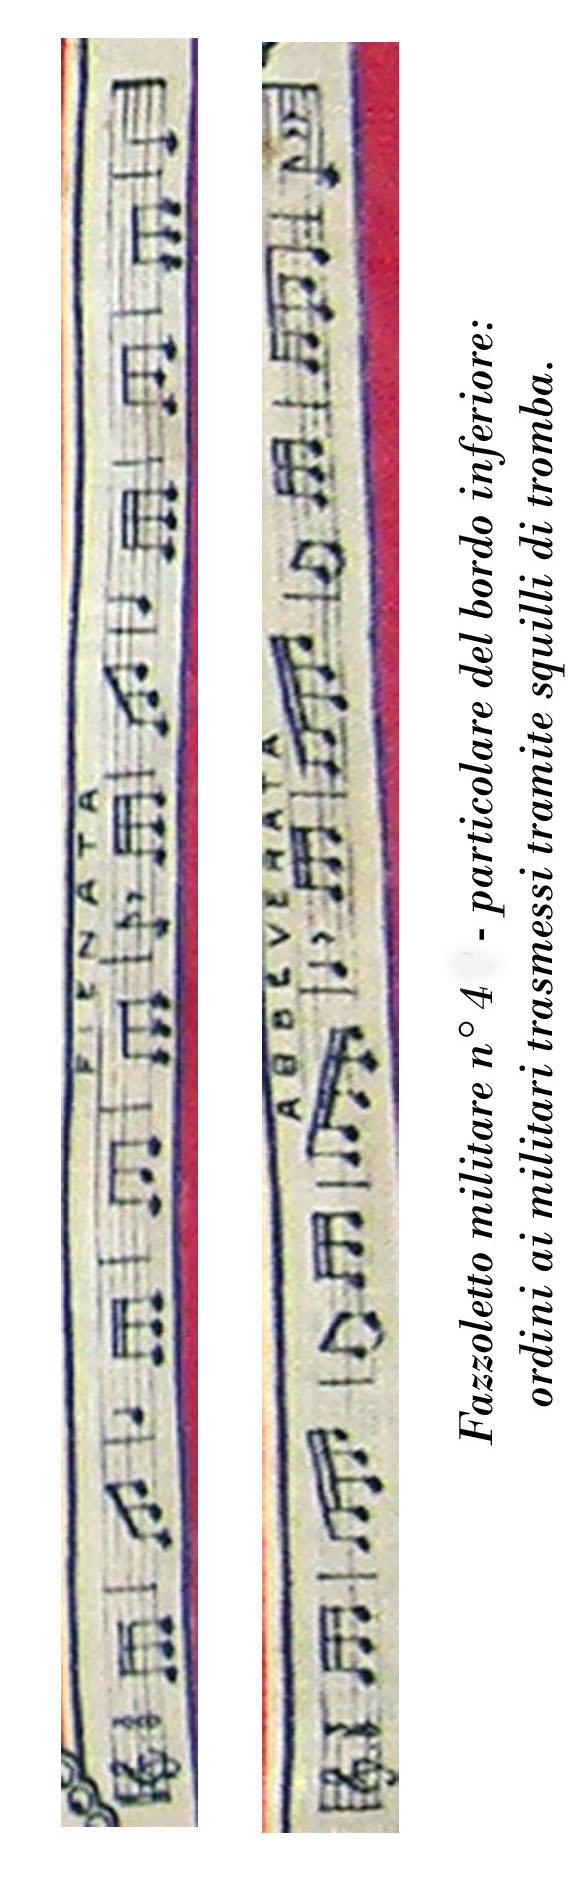
\includegraphics[width=\textwidth]{fazzoletto4_particolare_7.jpg}
	\caption{}
	\label{fig:fazzoletto4_particolare_7}
\end{figure}

\newpage

\begin{figure}[h]
	\centering
		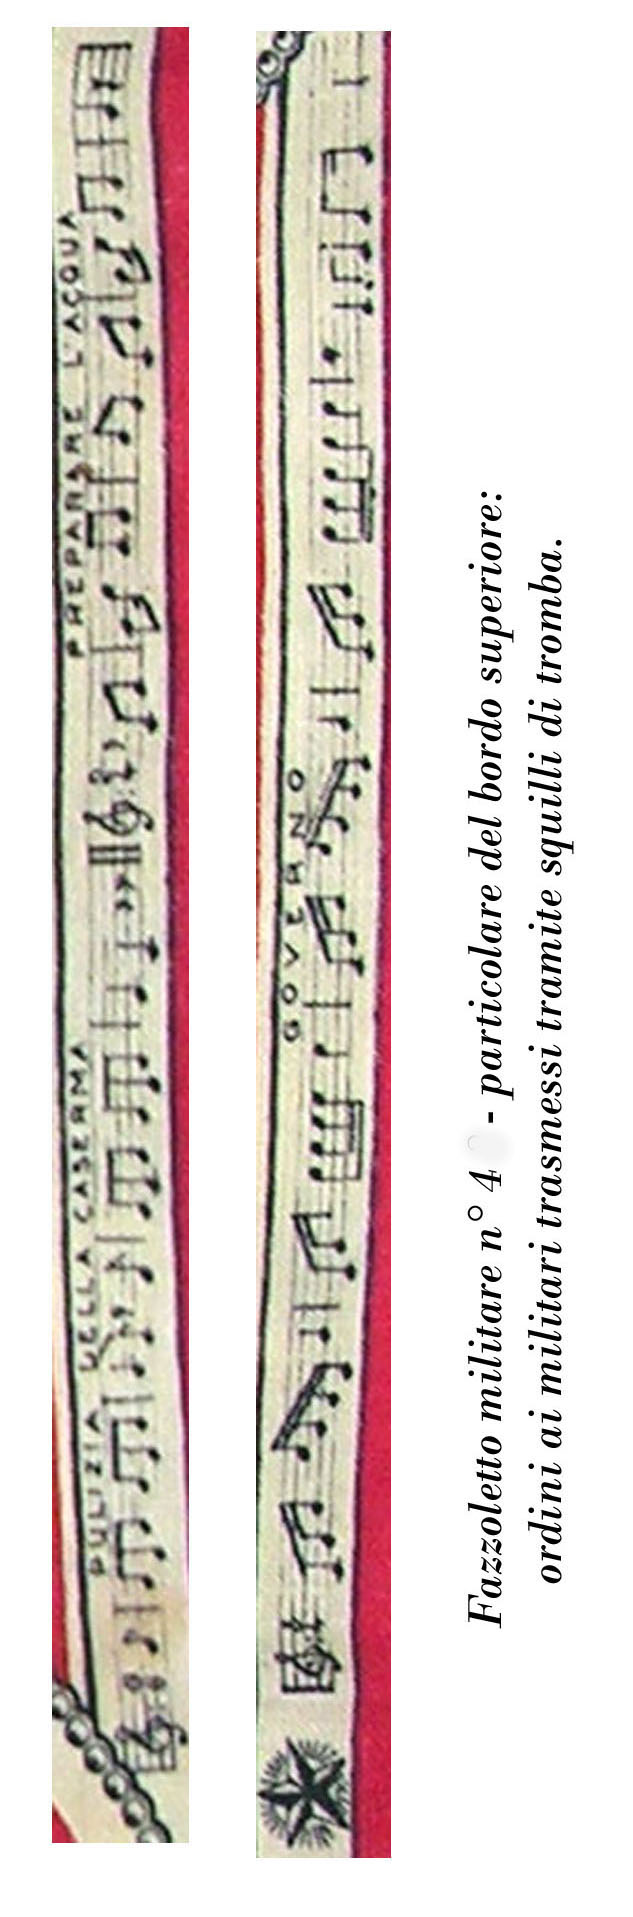
\includegraphics[width=\textwidth]{fazzoletto4_particolare_8.jpg}
	\caption{}
	\label{fig:fazzoletto4_particolare_8}
\end{figure}

\newpage

\begin{figure}[h]
	\centering
		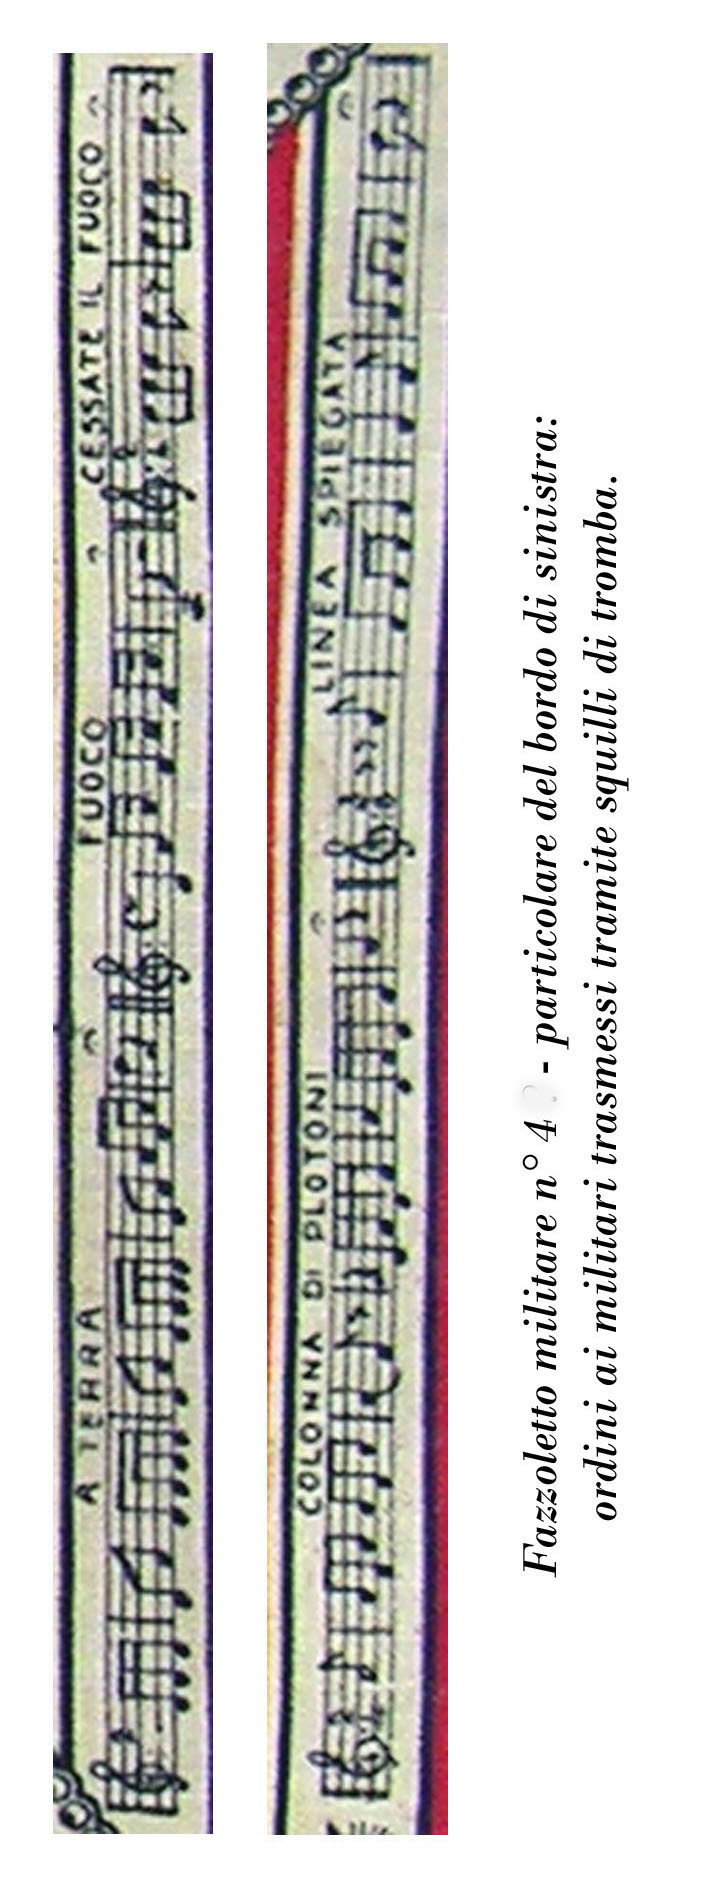
\includegraphics[width=\textwidth]{fazzoletto4_particolare_9.jpg}
	\caption{}
	\label{fig:fazzoletto4_particolare_9}
\end{figure}

\newpage

\begin{figure}[h]
	\centering
		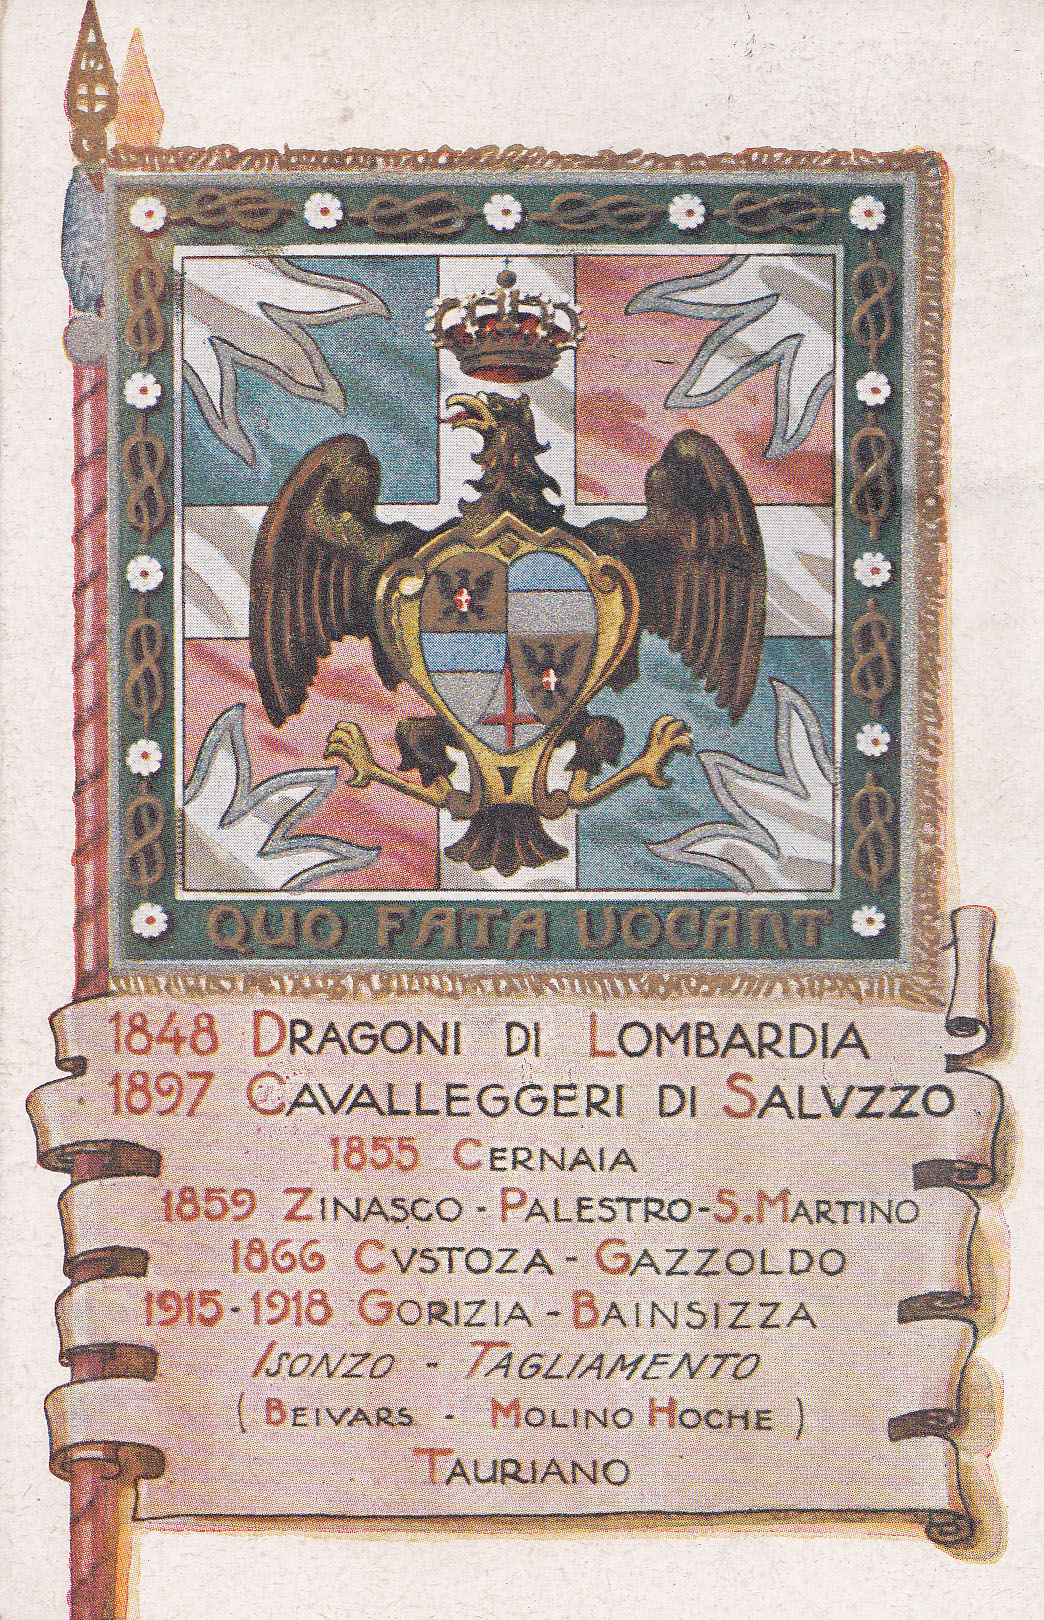
\includegraphics[width=\textwidth]{cartolina_dragoni.jpg}
	\caption{Cartolina emessa per l’Arma della Regia Cavalleria Periodo 1920-1930}
	\label{fig:cartolina_dragoni}
\end{figure}

\newpage

\begin{figure}[h]
	\centering
		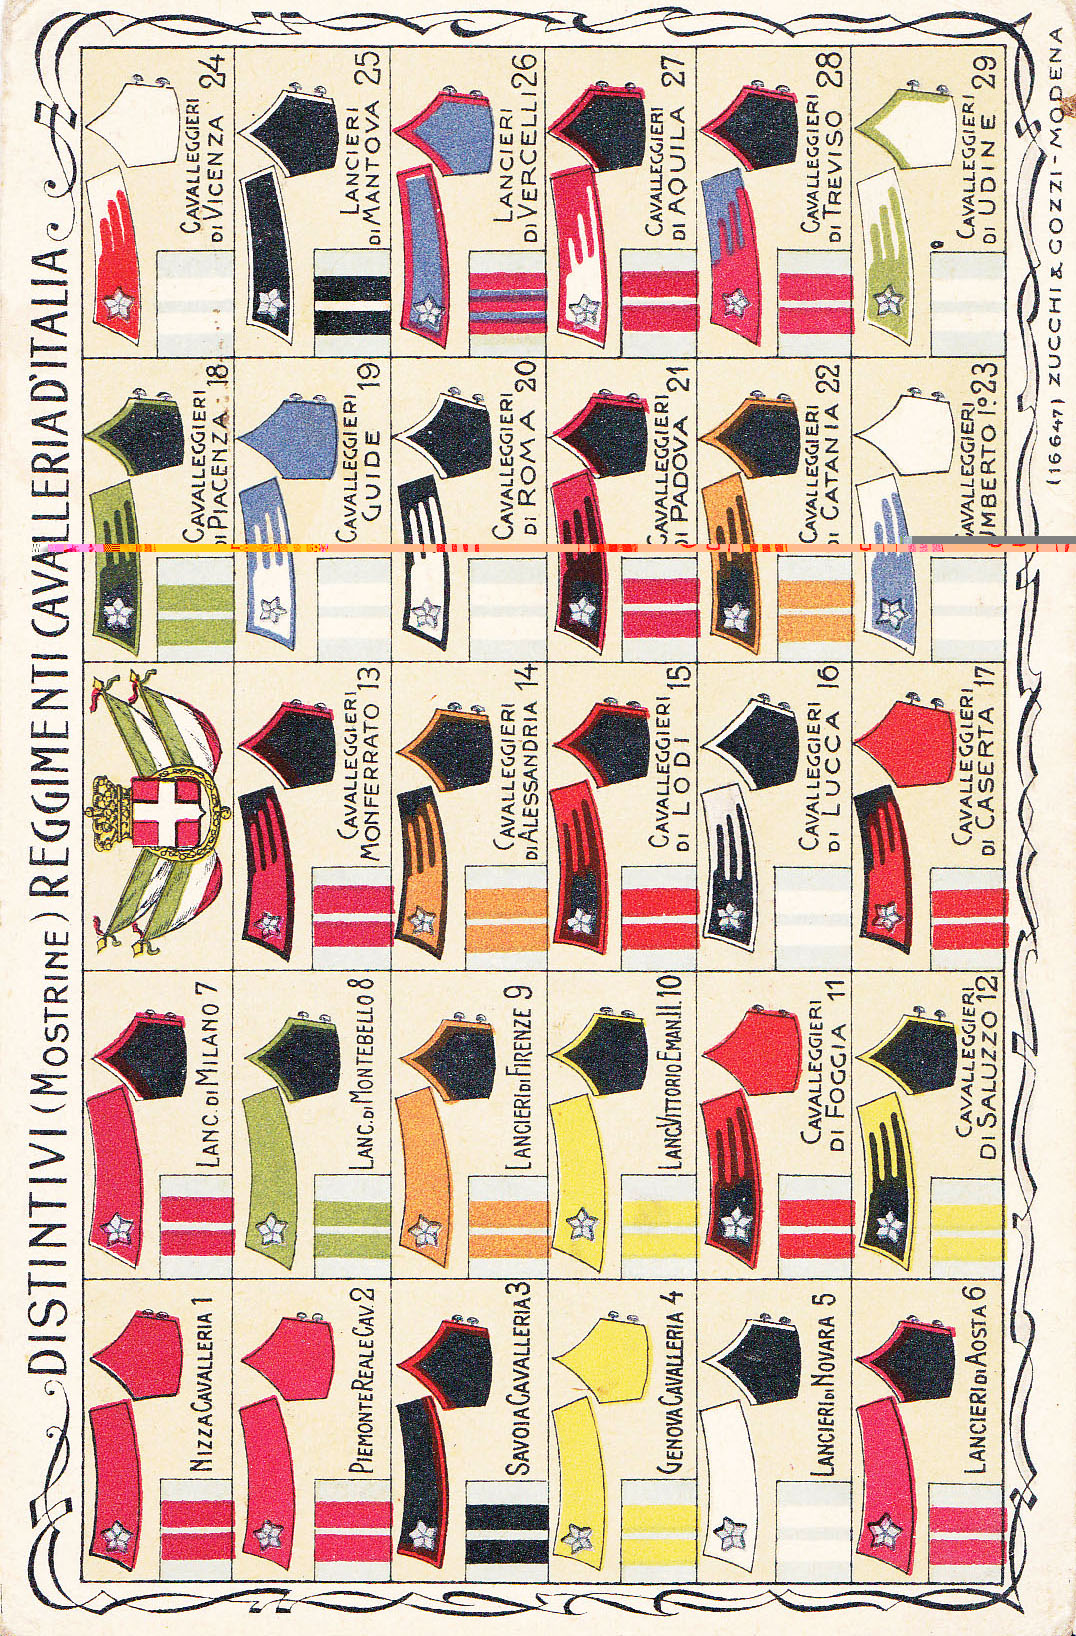
\includegraphics[width=\textwidth]{cartolina_regiacavalleria.jpg}
	\caption{Cartolina emessa per l’Arma della Regia Cavalleria Periodo 1920-1930}
	\label{fig:cartolina_regiacavalleria}
\end{figure}

\newpage

\begin{figure}[h]
	\centering
		
\includegraphics[width=\textwidth]{fazzoletto5_particolare.jpg}
	\caption{Particolare del fazzoletto militare n° 5. Stemma di Milano e numero degli abitanti della Provincia nel 1912}
	\label{fig:fazzoletto5_particolare}
\end{figure}

\newpage

Altre produzioni dell’epoca 1915-18 circa
    I due seguenti fazzoletti vennero prodotti probabilmente durante  il periodo della prima guerra mondiale. Il primo si riferisce all’igiene in ambito domestico. Il secondo è dedicato all’educazione civica. Le frasi riportate sono estrapolate da discorsi che Giuseppe Frua fece alle maestranze in occasione di incontri per ricorrenze o conferimento di attestati.
    
\begin{figure}[h]
	\centering
		\includegraphics[width=\textwidth]{fazzoletto_educazionefamiliare.jpg}
	\caption{Fazzoletto di educazione famigliare. Dimensioni: 25 x 25 cm}
	\label{fig:fazzoletto_educazionefamiliare}
\end{figure}

\newpage

\begin{figure}[h]
	\centering
		\includegraphics[width=\textwidth]{fazzoletto_educazionecivica.jpg}
	\caption{Fazzoletto di educazione civica  con scritte di Giuseppe Frua. Dimensioni: 27 x 27 cm}
	\label{fig:fazzoletto_educazionecivica}
\end{figure}

\newpage

\begin{figure}[h]
	\centering
		\includegraphics[width=\textwidth]{foulard_etiopia.jpg}
	\caption{Foulard Etiopia del 1935/36. Dimensioni: 78 x 75 cm}
	\label{fig:foulard_etiopia}
\end{figure}

Probabilmente questa produzione fu fatta per il contributo dato dall’Aeronautica militare italiana alla conquista di quel territorio. 

\newpage

\begin{figure}[h]
	\centering
		\includegraphics[width=\textwidth]{produzione_casalinga_tessuti.jpg}
	\caption{Produzione casalinga di tessuti fine “800 e inizi “900}
	\label{fig:produzione_casalinga_tessuti}
\end{figure}

\clearpage










































\clearpage
\chapter[]{Trame, stampe e disegni}
\graphicspath{ {./images/chapter4/} }

Questo capitolo raccoglie alcune significative immagini dei principali manufatti d’epoca pre-bellica e bellica del secondo conflitto mondiale.

\newpage

\begin{figure}[h]
	\centering
		\includegraphics[width=\textwidth]{tessuto1.jpg}
	\caption{}
	\label{fig:tessuto1}
\end{figure}








\clearpage

\clearpage
\chapter[]{Tessuti artificiali}
\graphicspath{ {./images/chapter5/} }

\begin{figure}[h]
	\centering
		\includegraphics[width=\textwidth]{tessilinuovi.jpg}
	\caption{Copertina della rivista trimestrale “I TESSILI NUOVI” n° 28  Luglio-Settembre 1941}
	\label{fig:tessilinuovi}
\end{figure}

\newpage

   La DAF negli anni ’30 del XX° secolo era all’apice del livello produttivo sia come qualità che quantità. Ma nel 1935 con la guerra d’Etiopia l’Italia si trovò a dover contrastare l’embargo delle materie prime voluto dalla Società delle Nazioni per iniziativa di Gran Bretagna e Francia.
   Nel campo tessile per far fronte alla penuria di materiale naturale vennero incrementate al massimo la ricerca e la produzione di fibre sintetiche . 
   Venivano così prodotti dei surrogati denominati Lanital, Terital, Rayon ecc… ecc….
   Tra le aziende produttrici di tessuti con questi materiali imposti dalla autarchia vi era la Snia Viscosa. 
   Questa industria pubblicava una rivista trimestrale che informava sulle iniziative aziendali e le attività produttive. Il titolo della pubblicazione era “I TESSILI NUOVI”. 
   Dal numero 28 del Luglio - Settembre 1941 e dal numero 31 dell’Aprile – Giugno 1942 di detto periodico apprendiamo che anche la DAF utilizzava tessuti SNIA per i propri stampati.
   Sempre su questi numeri viene riferito che la grande e milanesissima Sarta (a quei tempi si nominava così chi produceva alta moda) Biki utilizzava prodotti SNIA per le proprie creazioni. Accostando questi riferimenti è lecito supporre, anche se tuttora una conferma non l’abbiamo, che Biki per i suoi  lavori usasse prodotti DAF  con materiali sia sintetici che naturali. 

\newpage

\begin{figure}[h]
	\centering
		\includegraphics[width=\textwidth]{tessilinuovi_2.jpg}
	\caption{Dalla rivista “I TESSILI NUOVI” n° 28 – 1941  pag. 8}
	\label{fig:tessilinuovi_2}
\end{figure}

\newpage

\begin{figure}[h]
	\centering
		\includegraphics[width=\textwidth]{tessilinuovi_3.jpg}
	\caption{Dalla rivista “I TESSILI NUOVI”n° 31 Aprile-Giugno 1942 pag. 4}
	\label{fig:tessilinuovi_3}
\end{figure}

A piè di foto la scritta BIKI MILANO

\newpage

\begin{figure}[h]
	\centering
		\includegraphics[width=\textwidth]{tessilinuovi_4.jpg}
	\caption{Dalla Rivista “I TESSILI NUOVI”n° 28- 1941 pag. 11}
	\label{fig:tessilinuovi_4}
\end{figure}

\begin{figure}[h]
	\centering
		\includegraphics[width=\textwidth]{logo_snia.jpg}
	\caption{Logo  SNIA VISCOSA}
	\label{fig:logo_snia}
\end{figure}

\newpage

\begin{figure}[h]
	\centering
		\includegraphics[width=\textwidth]{biki.jpg}
	\caption{}
	\label{fig:biki}
\end{figure}

\newpage

\begin{figure}[h]
	\centering
		\includegraphics[width=\textwidth]{summer_fashon_1.jpg}
	\caption{}
	\label{fig:summer_fashon_1}
\end{figure}

\begin{figure}[h]
	\centering
		\includegraphics[width=\textwidth]{summer_fashon_2.jpg}
	\caption{}
	\label{fig:summer_fashon_2}
\end{figure}

\newpage

\begin{figure}[h]
	\centering
		\includegraphics[width=\textwidth]{ciclo_produzione_nylon.jpg}
	\caption{}
	\label{fig:ciclo_produzione_nylon}
\end{figure}

\newpage

\begin{figure}[h]
	\centering
		\includegraphics[width=\textwidth]{ciclo_produzione_raion.jpg}
	\caption{}
	\label{fig:ciclo_produzione_raion}
\end{figure}

\clearpage





\clearpage
\chapter[]{Tovaglie e tovaglioli}
\graphicspath{ {./images/chapter6/} }

Immagini di prodotti dal largo impiego in ambito domestico e familiare.

\newpage

\begin{figure}[h]
	\centering
		\includegraphics[width=\textwidth]{tovaglia_1.jpg}
	\caption{Tovaglia Dimensioni: cm 134 x 124-particolare-.}
	\label{fig:tovaglia_1}
\end{figure}

\newpage

\begin{figure}[h]
	\centering
		\includegraphics[width=\textwidth]{tovaglia_1_dettagli.jpg}
	\caption{La stessa tovaglia della pagina precedente con dettagli fronte e retro}
	\label{fig:tovaglia_1_dettagli}
\end{figure}

\newpage

\begin{figure}[h]
	\centering
		\includegraphics[width=\textwidth]{tovaglia_2.jpg}
	\caption{Tovaglia. Dimensioni: 250 x 136 cm -particolare-}
	\label{fig:tovaglia_2}
\end{figure}

\newpage

\begin{figure}[h]
	\centering
		\includegraphics[width=\textwidth]{pezza_di_prova.jpg}
	\caption{Pezza di prova per produzione di tovaglie e tovaglioli}
	\label{fig:pezza_di_prova}
\end{figure}

\newpage

\begin{figure}[h]
	\centering
		\includegraphics[width=\textwidth]{tovaglietta_prima_colazione.jpg}
	\caption{Tovaglietta da prima colazione. Dimensioni: 44 x 33 cm}
	\label{fig:tovaglietta_prima_colazione}
\end{figure}

\newpage

\begin{figure}[h]
	\centering
		\includegraphics[width=\textwidth]{grembiule_da_cucina.jpg}
	\caption{Grembiule da cucina}
	\label{fig:grembiule_da_cucina}
\end{figure}

\clearpage




\clearpage
\chapter[]{Strofinacci da cucina}
\graphicspath{ {./images/chapter7/} }

Una raccolta di immagini dei più utili e indispensabili strumenti di casa, spesso impreziositi da disegni pieni di buon gusto e allegria.

\newpage

\begin{figure}[h]
	\centering
		\includegraphics[width=\textwidth]{tovaglia_buon_natale_anno.jpg}
	\caption{}
	\label{fig:tovaglia_buon_natale_anno}
\end{figure}

\newpage

\begin{figure}[h]
	\centering
		\includegraphics[width=\textwidth]{tovaglia_salumi.jpg}
	\caption{}
	\label{fig:tovaglia_salumi}
\end{figure}

\newpage

\begin{figure}[h]
	\centering
		\includegraphics[width=\textwidth]{tovaglia_vaso_di_fiori.jpg}
	\caption{}
	\label{fig:tovaglia_vaso_di_fiori}
\end{figure}

\newpage

\begin{figure}[h]
	\centering
		\includegraphics[width=\textwidth]{tovaglia_teiere.jpg}
	\caption{}
	\label{fig:tovaglia_teiere}
\end{figure}

\newpage

\begin{figure}[h]
	\centering
		\includegraphics[width=\textwidth]{tovaglia_pesci.jpg}
	\caption{}
	\label{fig:tovaglia_pesci}
\end{figure}

\newpage

\begin{figure}[h]
	\centering
		\includegraphics[width=\textwidth]{tovaglia_arnesi.jpg}
	\caption{}
	\label{fig:tovaglia_arnesi}
\end{figure}

\newpage

\begin{figure}[h]
	\centering
		\includegraphics[width=\textwidth]{tovaglia_arnesi_2.jpg}
	\caption{}
	\label{fig:tovaglia_arnesi_2}
\end{figure}

\newpage

\begin{figure}[h]
	\centering
		\includegraphics[width=\textwidth]{tovaglia_galli.jpg}
	\caption{}
	\label{fig:tovaglia_galli}
\end{figure}

\newpage

\begin{figure}[h]
	\centering
		\includegraphics[width=\textwidth]{tovaglia_rose.jpg}
	\caption{}
	\label{fig:tovaglia_rose}
\end{figure}


\clearpage



\clearpage
\chapter[]{Pubblicità promozione e immagine}
\graphicspath{ {./images/chapter8/} }

La DAF ha propagandato la propria produzione in svariate forme ma soprattutto sui periodici di moda femminile: Vesta, Vendere, Mani di Fata. I prodotti lavorati erano cotone, satin, taffettà, materassè, seta da paracadute, seta pura italiana, georgette. Il marchio di fabbrica era “Sole Onda”, come riportato in figura. 

\begin{figure}[h]
	\centering
		\includegraphics[width=\textwidth]{marchio_daf.jpg}
	\caption{Marchio di fabbrica della DAF}
	\label{fig:marchio_daf}
\end{figure}

I nomi originali dei principali prodotti erano: Telene (tela), Sol (cretonnè), Costella (tessuto per abiti), Velita (voilè a doppio ritorto per abiti), Radiosa (seta artificiale per abiti), Tuxo (rayon, fibra artificiale), Retex (seta e lana).

\newpage

\begin{figure}[h]
	\centering
		\includegraphics[width=\textwidth]{mani_di_fata.jpg}
	\caption{}
	\label{fig:mani_di_fata}
\end{figure}

\newpage

\begin{figure}[h]
	\centering
		\includegraphics[width=\textwidth]{tuxo.jpg}
	\caption{Da ”Mani di Fata” del dicembre 1932  n° 12}
	\label{fig:tuxo}
\end{figure}

\newpage

\begin{figure}[h]
	\centering
		\includegraphics[width=\textwidth]{tessuti_stampati.jpg}
	\caption{Pagina pubblicitaria per tessuti stampati}
	\label{fig:tessuti_stampati}
\end{figure}

\newpage

\begin{figure}[h]
	\centering
		\includegraphics[width=\textwidth]{pagina_pubblicitaria_fioclin.jpg}
	\caption{Pagina pubblicitaria del 1938}
	\label{fig:pagina_pubblicitaria_fioclin}
\end{figure}

\newpage

\begin{figure}[h]
	\centering
		\includegraphics[width=\textwidth]{telene.jpg}
	\caption{Da “Mani di Fata” dell’ agosto 1931, pag. 19}
	\label{fig:telene}
\end{figure}

\newpage

\begin{figure}[h]
	\centering
		\includegraphics[width=\textwidth]{radiosa.jpg}
	\caption{Da “L’illustrazione italiana” n° 22 del  giugno 1930, pag. 978}
	\label{fig:radiosa}
\end{figure}

\newpage

\begin{figure}[h]
	\centering
		\includegraphics[width=\textwidth]{radiosa_tuxo.jpg}
	\caption{Da “Mani di Fata” del luglio 1932, pag. 15}
	\label{fig:radiosa_tuxo}
\end{figure}

\newpage

\begin{figure}[h]
	\centering
		\includegraphics[width=\textwidth]{vestite_di_tuxo.jpg}
	\caption{Da “Mani di Fata” dell’agosto 1932, pag. 19}
	\label{fig:vestite_di_tuxo}
\end{figure}

\newpage

\begin{figure}[h]
	\centering
		\includegraphics[width=\textwidth]{la_moda.jpg}
	\caption{}
	\label{fig:la_moda}
\end{figure}

\newpage

\begin{figure}[h]
	\centering
		\includegraphics[width=\textwidth]{locandina.jpg}
	\caption{Locandina tranviaria}
	\label{fig:locandina}
\end{figure}

\newpage

\begin{figure}[h]
	\centering
		\includegraphics[width=\textwidth]{biancaneve.jpg}
	\caption{Produzione di fazzoletti con personaggi Walt Disney}
	\label{fig:biancaneve}
\end{figure}
\begin{figure}[h]
	\centering
		\includegraphics[width=\textwidth]{boccasile.jpg}
	\caption{Cartolina a firma Boccasile}
	\label{fig:boccasile}
\end{figure}

\newpage

Serie di sei cartoline pubblicitarie emesse nel 1939

\begin{figure}[h]
	\centering
		\includegraphics[width=\textwidth]{cartolina_1.jpg}
	\caption{}
	\label{fig:cartolina_1}
\end{figure}
\begin{figure}[h]
	\centering
		\includegraphics[width=\textwidth]{cartolina_2.jpg}
	\caption{}
	\label{fig:cartolina_2}
\end{figure}

\newpage

\begin{figure}[h]
	\centering
		\includegraphics[width=\textwidth]{cartolina_3.jpg}
	\caption{}
	\label{fig:cartolina_3}
\end{figure}
\begin{figure}[h]
	\centering
		\includegraphics[width=\textwidth]{cartolina_4.jpg}
	\caption{}
	\label{fig:cartolina_4}
\end{figure}

\newpage

\begin{figure}[h]
	\centering
		\includegraphics[width=\textwidth]{cartolina_5.jpg}
	\caption{}
	\label{fig:cartolina_5}
\end{figure}
\begin{figure}[h]
	\centering
		\includegraphics[width=\textwidth]{cartolina_6.jpg}
	\caption{}
	\label{fig:cartolina_6}
\end{figure}

\newpage

\begin{figure}[h]
	\centering
		\includegraphics[width=\textwidth]{cartolina_finale.jpg}
	\caption{Stampigliatura sul retro delle sei  cartoline pubblicitarie}
	\label{fig:cartolina_finale}
\end{figure}

\newpage

\begin{figure}[h]
	\centering
		\includegraphics[width=\textwidth]{deangeli_1.jpg}
	\caption{}
	\label{fig:deangeli_1}
\end{figure}
\begin{figure}[h]
	\centering
		\includegraphics[width=\textwidth]{deangeli_2.jpg}
	\caption{}
	\label{fig:deangeli_2}
\end{figure}
\begin{figure}[h]
	\centering
		\includegraphics[width=\textwidth]{deangeli_3.jpg}
	\caption{}
	\label{fig:deangeli_3}
\end{figure}


\clearpage

\clearpage
\chapter[]{RIFERIMENTI}

Dal periodico della Snia Viscosa 1938-1942. Numeri vari
RIFERIMENTI


Ideatore dell’opera: 	                          	  Loredano Tavazzi
Elaborazione immagini e inserimento testi:
     Giancarlo Soave
            Niccolò Zucchi Frua
Impostazione, coordinamento, ricerca, 
scelta immagini e didascalie:                          Loredano Tavazzi                                     



I documenti per i fazzoletti di istruzione militare provengono dall’archivio del Dott. Dirk Ziesing

Tutti gli altri documenti provengono dall’archivio 
 Loredano Tavazzi



Per le traduzioni da tedesco, francese e inglese hanno contribuito:

 Alessandro Porro, 		docente dell’Università di Brescia
Cinzia Pozzi. 						     interprete
Carlo Solarino , 					    giornalista 	







AUTORI DEI TESTI

- Marina Frua -
Premessa


-Dirk Ziesing- 
Military instruction hanndkerchief of the British Empire
Italien- De Angeli Frua


-Loredano Tavazzi -
Estrapolazioni dai testi originali di Dirk Ziesing e di alcuni significativi particolari dai singoli manufatti.
Note esplicative su fazzoletti cavalleria e armi pesanti.
Note esplicative su fazzoletti 1915–1918.
Nota esplicativa sul foulard Etiopia.
Nota esplicativa sui tessuti artificiali.
Note esplicative su pubblicità e promozione.



INDICE DEI TESTI E ARGOMENTI

Premessa 						         pag.   5

Capitolo I
La nascita dei fazzoletti  per  istruzione militare          pag.    7                                  
Military instruction handkerchief
		of the British Empire  				       pag.      8
I fazzoletti con istruzioni militari dell’Impero Britannico  							                    pag.     9                                                        
Il primo fazzoletto britannico con istruzioni                 pag.  11
Il secondo  fazzoletto britannico con istruzioni             pag.  17
Il terzo  fazzoletto britannico con istruzioni                   pag. 25
L’origine dei fazzoletti con istruzioni militari               pag. 31


Capitolo II
I fazzoletti per istruzione militare in Italia 
prima parte: descrizione storica                                  pag.  37                                                        
  De Angeli Frua                                      		         pag.  39
Sguardo d’insieme     			  	          pag. 39
Il fazzoletto italiano n°1	                   		          pag. 39
Il fazzoletto italiano n°2                           		          pag. 43
Il fazzoletto italiano n°3	                      		          pag. 43
Il fazzoletto italiano con carta geografica del 1912         pag. 59
Il fazzoletto italiano con carta geografica del 1918         pag. 61
I rapporti tra Francia e Italia	                    		          pag. 61

Capitolo III
I fazzoletti per istruzione militare in Italia - Seconda parte                                                                                           pag. 65                                                                            pag.   65                           
De Angeli Frua			               	          pag. 66
Sguardo d’insieme			         		         pag.  67
Il fazzoletto italiano n° 1                              	         pag.  68 
Il fazzoletto italiano n° 2                               	         pag.  68
Il fazzoletto italiano n° 3                              	         pag.  69
Fazzoletto cartografico italiano del 1912      	         pag.  70
Fazzoletto cartografico italiano del 1918       	          pag. 72
Nota esplicativa                                             	         pag.  72
Altre produzioni dell’epoca                          	         pag.  95
Specifica su fazzoletto Etiopia 1935-36 		         pag.  97

Capitolo IV 
Tessuti disegni e trame del periodo 1930-1943               pag. 99
Capitolo V
Tessuti artificiali del periodo 1938-1943             	        pag. 109
Capitolo VI
Tovaglie, tovaglioli e altro del periodo 1950-1965        pag. 119    
Capitolo VII
Strofinacci da cucina  del periodo  1965-1970               pag. 127                                             
Capitolo VIII
Pubblicità, promozioni, immagine 		 	        pag. 137
Specifica sulla pubblicità  				       pag.  138

Riferimenti		           			        pag. 155
Autori dei testi				                    pag. 156
INDICE DELLE ILLUSTRAZIONI

Ciclo di lavorazione della seta, anno 1933  	          pag.   2
Prima pagina della rivista inglese sulla 
nascita dei fazzoletti di istruzione militare   	          pag. 12                              
Fazzoletto militare britannico n°1		                     pag.  13
Particolari del fazzoletto n°1   		                pag. 14-15
Fazzoletto militare britannico n°2 		                     pag.  18
Particolare del fazzoletto n°2  		                     pag.  19
Fazzoletto militare britannico della marina n°3           pag. 22
Fazzoletto britannico della Marina -particolare 	          pag. 23
Fazzoletto militare italiano n°1                                    pag.   40
Fazzoletto militare italiano n°2                                     pag.  41
Particolare del fazzoletto militare italiano n°2A         pag.  44
Fazzoletto militare italiano n°3                                     pag.  45      
Fazzoletto militare italiano n°4 –Cavalleria-     	          pag. 52
Fazzoletto delle armi pesanti                   		          pag. 53
Fazzoletto militare italiano n°5 cartografico 1912       pag. 56
Fazzoletto militare italiano n°6 cartografico 1918       pag. 57
Dettaglio in basso a sinistra del fazzoletto n°1              pag. 62
Documento descrizione contenuti fazzoletto n°1          pag. 63
Richiesta di G. Frua per stampa fazzoletti militari      pag. 64
Certificazione della produzione De Angeli                     pag. 73
Particolari del fazzoletto militare italiano n°2   pag. 73-75-76
Particolare del fazzoletto militare italiano n°1            pag.  74
Particolari del fazzoletto militare italiano n°2A    pag.77 a 81
Fazzoletto militare italiano n°4 per Cavalleria             pag. 80
Particolari del fazzoletto militare italiano n°4           pag. 81-83          
Particolare del fazzoletto militare italiano n°3   pag. da 82 a 84     
Particolari del fazzoletto militare italiano n°4         pag. 88-91        
Cartoline della Regia Cavalleria 1920-1930              pag. 92-93
Particolare del fazzoletto militare italiano n°5            pag.  94    
Fazzoletto di educazione famigliare                              pag.  95
Fazzoletto di educazione civica                                     pag.  96
Foulard  della guerra d’Etiopia 1935-1936                   pag.  97
Produzione tessile di fine ‘800                                        pag.  98
Disegni di tessuti                                                     pag. 100-108
“I tessili nuovi” 1941, copertina                                   pag. 110
“I tessili nuovi” 1941, pagine interne                     pag. 112-114
Logo Snia Viscosa                                                          pag. 114
La stilista Biki (da Corsera)                                          pag. 115
Ciclo di produzione del nylon                                        pag. 116
Ciclo di produzione del nàion e del fiocco                     pag. 117
Particolari tovaglie                                                 pag. 120-122
Prove produzione tovaglie e tovaglioli                         pag. 123
Tovaglietta per prima colazione                                   pag. 124
Grembiule da cucina                                                      pag. 125
Strofinacci da cucina                                             pag. 128-136
Intestazione “Mani di fata”                                          pag. 139
Intestazione “L’illustrazione italiana”                         pag. 139
“Mani di fata”, pagine interne                               pag. 140-142
Locandina tramviaria                                                    pag. 143
Fazzoletti con personaggi W. Disney                           pag. 144
Cartoline                                                                  pag. 144-148
Pagine e immagini pubblicitarie                            pag. 149-154


\clearpage

\clearpage

\end{document}
